\documentclass[11pt,a4paper]{article}
\ifdefined\pdfinfoomitdate\pdfinfoomitdate=1\fi
\ifdefined\pdftrailerid\pdftrailerid{}\fi
\ifdefined\pdfsuppressptexinfo\pdfsuppressptexinfo=15\fi
\usepackage[T1]{fontenc}
\usepackage{lmodern}
\usepackage[margin=28mm]{geometry}
\usepackage{amsmath,amssymb,amsthm,mathtools}
\usepackage{microtype,enumitem,booktabs,array,tikz}
\usetikzlibrary{arrows.meta,positioning}
\usepackage[hidelinks]{hyperref}
\numberwithin{equation}{section}
\newtheorem{theorem}{Theorem}[section]
\newtheorem{lemma}[theorem]{Lemma}
\newtheorem{proposition}[theorem]{Proposition}
\newtheorem{corollary}[theorem]{Corollary}
\theoremstyle{definition}
\newtheorem{definition}[theorem]{Definition}
\theoremstyle{remark}
\newtheorem{remark}[theorem]{Remark}
\newcommand{\C}{\mathbb C}
\newcommand{\R}{\mathbb R}
\newcommand{\N}{\mathbb N}
\newcommand{\T}{\operatorname T}
\newcommand{\U}{\mathcal U}
\newcommand{\Tr}{\operatorname{Tr}}
\newcommand{\tr}{\operatorname{tr}}
\newcommand{\dist}{\operatorname{dist}}
\newcommand{\her}{\operatorname{her}}
\newcommand{\Her}{\operatorname{her}}
\newcommand{\supp}{\operatorname{supp}}
\newcommand{\id}{\operatorname{id}}
\newcommand{\rr}{\operatorname{rr}}
\newcommand{\eps}{\varepsilon}
\DeclarePairedDelimiter{\norm}{\lVert}{\rVert}
\newcommand{\normtwo}[2]{\left\|#1\right\|_{2,#2}}
\newcommand{\normone}[2]{\left\|#1\right\|_{1,#2}}
\newcommand{\Z}{\mathcal Z}
\newcommand{\Zalg}{\mathcal Z}
\newcommand{\K}{\mathcal K}
\newcommand{\Oinf}{\mathcal O_{\infty}}
\newcommand{\one}{\mathbf1}
\newcommand{\Aw}{A^\omega}
\newcommand{\Aom}{A_\omega}
\newcommand{\Fw}{F_\omega(A)}
\DeclareMathOperator{\sgn}{sgn}
\DeclareMathOperator{\Cu}{Cu}
\DeclareMathOperator{\Ped}{Ped}
\setlength{\emergencystretch}{2em}
\hypersetup{pdftitle={Tracial projection methods and uniform property Gamma},pdfauthor={OpenAI},pdfsubject={Real rank zero, nuclearity and uniform central trace splitting}}
\title{Tracial projection methods and uniform property \(\Gamma\)}
\author{OpenAI}
\date{September 23, 2026}
\begin{document}
\maketitle
\begin{abstract}
For a simple, separable, unital, infinite-dimensional, nuclear, stably finite
$C^*$-algebra with traces, real rank zero of the uniform tracial ultrapower
of its uniform tracial completion implies uniform property $\Gamma$.
This answers Problem XXI of Schafhauser, Tikuisis and White affirmatively.
Independently, strict comparison implies Jiang--Su absorption for simple,
separable, unital, infinite-dimensional nuclear algebras, resolving the
unital Toms--Winter conjecture. Under comparison tested on traces of finite
target rank, we also obtain uniform property $\Gamma$ and absorption for
simple, separable, nuclear, stably projectionless algebras whose densely
finite traces are all bounded and have a nonempty compact normalized base.
\end{abstract}
\tableofcontents
\section{Introduction}\label{sec:introduction}

Uniform property $\Gamma$ asks for central projections that divide every
trace while preserving its values on prescribed coefficients. This form of
central divisibility is central to the regularity theory of nuclear
$C^*$-algebras. It was introduced by Castillejos, Evington, Tikuisis, White
and Winter \cite[Definition~2.1]{CETWW}, and developed systematically by
Castillejos, Evington, Tikuisis and White \cite{CETW}. For simple separable
unital nuclear algebras with traces, strict comparison together with uniform
property $\Gamma$ is equivalent to absorption of the Jiang--Su algebra
\cite[Theorem~5.6]{CETW}. We give three independent constructions of this central divisibility.
The first derives uniform property $\Gamma$ from real rank zero of a
completion ultrapower, answering a question of Schafhauser, Tikuisis and
White. The second derives Jiang--Su absorption from strict comparison
in the unital setting, completing the unital Toms--Winter equivalence.
The third treats stably projectionless algebras with bounded densely
finite traces and a compact normalized trace base. The common task is
to make projections central while preserving every coefficient trace;
the hypotheses and the averaging arguments differ in the three routes.

The underlying finite-factor notion goes back to Murray and von Neumann
\cite{MurrayVonNeumann1943}. Dixmier developed its central projection
formulation \cite{Dixmier1969}, while McDuff studied the stronger central
matrix structure associated with absorption of the hyperfinite factor
\cite{McDuff1970}. Connes' classification of injective factors
\cite{Connes} supplies the pointwise von Neumann regularity used in our
nonunital construction. The uniform $C^*$-algebraic question asks for a
single family of projections that works simultaneously across the trace
space and retains every coefficient identity. Pointwise tracial
approximation must therefore be combined with a uniform construction.

The first construction starts with real rank zero in a uniform tracial
ultrapower. A unital $C^*$-algebra has \emph{real rank zero} when its
selfadjoint elements can be approximated in norm by selfadjoint elements
with finite spectrum \cite{BP91}. We first describe precisely
the resulting trace identities. For a unital algebra $A$ with nonempty
tracial-state space $T(A)$, put
\[
 \|a\|_{2,T(A)}=\sup_{\tau\in T(A)}\tau(a^*a)^{1/2}.
\]
The uniform tracial completion belongs to the framework initiated by
Ozawa \cite{Ozawa13} and developed in \cite{CCEGSTW}.
The algebra $B=\overline A^{T(A)}$ consists of bounded
uniformly $2$-Cauchy sequences modulo sequences tending to zero in this
seminorm. Each $\tau\in T(A)$ extends to a designated trace $\bar\tau$ on $B$.
For a fixed free ultrafilter $\omega$ on $\N$, the uniform tracial ultrapower
$B^\omega$ is the quotient of bounded sequences in $B$ by those whose uniform
$2$-norm tends to zero along $\omega$. The family $\Lambda_\omega$ consists
of exactly the traces
\[
 \lambda([(b_j)])=\lim_{j\to\omega}\bar\tau_j(b_j),
 \qquad \tau_j\in T(A).
\]
These constructions and their quotient norms are specified in
Section~\ref{r:sec:preliminaries}.

\begin{theorem}[Real rank zero and uniform property $\Gamma$]
\label{r:thm:main}
Let $A$ be a unital, separable, simple, infinite-dimensional, nuclear,
stably finite $C^*$-algebra with $T(A)\ne\varnothing$, and let
$B=\overline A^{T(A)}$. Fix any free ultrafilter $\omega$ on $\N$.
If $B^\omega$ has real rank zero in its quotient $C^*$-norm, then there is
a projection $p\in B^\omega\cap B'$ such that
\[
 \lambda(px)=\tfrac12\lambda(x)
 \qquad(x\in B,\ \lambda\in\Lambda_\omega).
\]
In particular, $A$ has uniform property $\Gamma$.
\end{theorem}

This gives a positive resolution of Problem~XXI of Schafhauser, Tikuisis
and White \cite[Section~6]{STW}. Their Definition~16 uses precisely this
completion and halving formulation. In the usual formulation, uniform
property $\Gamma$ requires, for every $m\ge1$, orthogonal projections
$p_1,\ldots,p_m\in A^\omega\cap A'$ summing to one such that
\[
 \lambda(ap_i)=\frac1m\lambda(a)
 \quad(a\in A,\ \lambda\in T_\omega(A)).
\]
Here $A^\omega$ is the uniform tracial ultrapower formed directly from $A$,
and $T_\omega(A)$ is its family of varying limit traces. The completion
formulation and the all-$m$ formulation agree by
\cite[Propositions~5.7, 5.20 and 5.23]{CCEGSTW}; we record the interfaces
beside the definitions in Section~\ref{r:sec:preliminaries}. The coefficient $a$ is essential: equality
of scalar traces of the $p_i$ alone does not give uniform property $\Gamma$.

The additional centrality in Theorem~\ref{r:thm:main} is the main issue.
Vaccaro derives tracial almost divisibility from real rank zero of the
tracial ultrapower: hereditary subalgebras admit tracially large matrix
order-zero maps, without a centrality requirement
\cite[Proposition~2.2]{Vac26}. Combined with tracially locally finite nuclear
dimension, this yields uniform McDuffness and hence uniform property
$\Gamma$ \cite[Theorem~2.3]{Vac26}. Kessinger and Toms obtain uniform
property $\Gamma$ from subquadratic growth in recursive-subhomogeneous
inductive limits and from a tracial local approximation condition
\cite[Theorems~1.2 and 7.11]{KT26}. Their results exclude nonzero
finite-dimensional representations; the local theorem also assumes
nonempty traces. Their argument supplies both ultrapower real rank zero
and tracially locally finite nuclear dimension, then uses this divisibility
route. We instead construct central coefficient splittings using
nuclear averaging under the hypotheses of Theorem~\ref{r:thm:main}.
Nuclearity alone does not ensure uniform property $\Gamma$: Toms constructs
a simple separable unital AH algebra without it \cite[Theorem~1]{Toms26}.

There are also implications in the other direction. For simple separable
unital infinite-dimensional nuclear algebras with traces, Fu proves that
uniform property $\Gamma$ implies the real-rank and divisibility
conditions of \cite[Theorems~1.1 and 10.6]{Fu26}.
Uniform property $\Gamma$ also passes to the tracial completion and
supplies complemented partitions of unity
\cite[Proposition~5.20 and Theorem~1.4]{CCEGSTW}.
For factorial tracially complete algebras, complemented partitions of unity
imply real rank zero of their tracial ultrapowers
\cite[Proposition~7.2]{CCEGSTW}; Evington and Tikuisis strengthen this to
real rank zero of the tracially complete algebra itself
\cite[Theorem~A]{EvingtonTikuisis26}. These results assume the uniform
partition structure from which projections can be assembled.
Theorem~\ref{r:thm:main} constructs central splittings from the ultrapower
real-rank-zero assumption.

The same hypotheses also identify all traces on the completion.

\begin{corollary}[Traces on the completion]\label{r:cor:completion-traces}
Under the hypotheses of Theorem~\ref{r:thm:main}, including real rank zero
of $B^\omega$ in its quotient $C^*$-norm, every tracial state of $B$ is
the designated extension of a unique trace in $T(A)$. Thus restriction
is an affine homeomorphism $T(B)\to T(A)$, with inverse
$\tau\mapsto\bar\tau$. Moreover,
\[
 |\sigma(b)|\le\|b\|_{2,T(A)}
 \qquad(b\in B,\ \sigma\in T(B)),
\]
so every tracial state of $B$ is continuous for the designated uniform
$2$-norm.
\end{corollary}

The proof appears at the end of Section~\ref{r:sec:completion}.

The construction is useful outside an ultrapower. A projection is called
\emph{full} when the closed two-sided ideal it generates is the entire
ambient algebra.

\begin{theorem}[Finite-set central splitting]\label{r:thm:finite}
Let $A\subseteq D$ be a unital inclusion of $C^*$-algebras, with $A$ nuclear,
$D$ of real rank zero, and $T(D)\ne\varnothing$. Suppose that for every
$\delta>0$ there is a full projection $g\in D$ with
$\sup_{\tau\in T(D)}\tau(g)<\delta$.
For every finite $K\subseteq\mathcal U(A)$ and $\varepsilon>0$ there is a
projection $P\in D$ such that, for every $x\in K$,
\[
 \sup_{\tau\in T(D)}\|[P,x]\|_{2,\tau}<\varepsilon,
 \qquad
 \sup_{\tau\in T(D)}|\tau(Px)-\tfrac12\tau(x)|<\varepsilon.
\]
\end{theorem}

The ambient algebra in this result need not be nuclear or simple. Its
tracial states need not be faithful. In the application $D=B^\omega$,
simplicity and infinite dimensionality of $A$ provide the full projections
of small trace uniformly over \emph{all} abstract tracial states of $D$.
The last diagonal argument then uses the specified family
$\Lambda_\omega$ to obtain a single projection commuting with all of $B$.

\subsection{Strict comparison and Jiang--Su absorption}

The next two results obtain uniform property $\Gamma$ directly from
strict comparison. Each supplies its own projections and is independent
of the real-rank-zero hypothesis in Theorem~\ref{r:thm:main}.
For positive $a,b\in A\otimes\K$, Cuntz subequivalence $a\precsim b$ means
that $x_n^*bx_n\to a$ in norm for a sequence $x_n\in A\otimes\K$.
Here $\K$ denotes the compact operators, tensor products are spatial,
and each trace is extended using the unnormalized matrix trace. Set
\[
 d_\tau(a)=\lim_{n\to\infty}(\tau\otimes\Tr)(a^{1/n})\in[0,\infty].
\]
For simple unital algebras we use the comparison convention
\[
 b\ne0,\quad d_\tau(a)<d_\tau(b)\ (\tau\in T(A))
 \quad\Longrightarrow\quad a\precsim b.
\]
If $T(A)$ is empty, this convention requires comparison with every nonzero
positive target; it is more than the absence of traces.

The Jiang--Su algebra $\Z$ was introduced by Jiang and Su \cite{JS};
$\Z$-stability means $A\cong A\otimes\Z$. For simple, separable,
unital, infinite-dimensional nuclear algebras, the Toms--Winter
conjecture asks for the equivalence \cite[Conjecture~9.3]{WZNuc}
\[
 \text{finite nuclear dimension}
 \quad\Longleftrightarrow\quad
 \mathcal Z\text{-stability}
 \quad\Longleftrightarrow\quad
 \text{strict comparison}.
\]
Finite nuclear dimension requires completely positive approximations
through finite-dimensional algebras with a fixed finite number of
outgoing pieces that preserve orthogonality of positive elements.
The implications from finite nuclear dimension to $\Z$-stability,
from $\Z$-stability to strict comparison, and from $\Z$-stability to
finite nuclear dimension are known \cite{WinterNuc,Rordam,CETWW}.
Theorem~\ref{u:thm:main} proves the remaining comparison-to-absorption
implication, giving a positive resolution in the unital setting.
The empty-trace case is included with the comparison convention stated
above; its purely infinite absorption argument is given in
Section~\ref{u:sec:gamma}.

\begin{theorem}[The direct unital comparison route]\label{u:thm:main}
Let $A$ be a simple, separable, unital, infinite-dimensional nuclear
$C^*$-algebra with strict comparison in the preceding sense.
Then $A\cong A\otimes\Z$. When $T(A)\ne\varnothing$, the proof constructs
uniform property $\Gamma$ directly.
\end{theorem}

In the tracial case, Matui and Sato established the absorption implication
for finitely many extremal traces using comparison and property~(SI)
\cite[Theorem~1.1]{MS}.
The compact finite-dimensional boundary case was obtained independently
by Kirchberg and R\o rdam \cite[Corollary~7.9]{KR14}, Sato
\cite[Corollary~1.2]{Sato12}, and Toms, White and Winter
\cite[Corollary~4.7]{TWW15}. Later results reach other trace spaces: Lin
proves the implication under his condition~(C) together with stable rank
one, and removes the stable-rank assumption in its countable-boundary case
\cite[Theorem~5.6 and Corollary~5.7]{Lin24}. Condition~(C) decomposes the
extreme boundary into countably many finite-dimensional compact pieces
with additional compatibility requirements on their convex faces
\cite[Definition~2.13]{Lin24}. Evington and Schafhauser subsequently
obtained uniform property $\Gamma$ from fibrewise property $\Gamma$
under the compact finite-dimensional boundary hypothesis without assuming
nuclearity \cite[Theorem~1.1]{EvingtonSchafhauser26}. The uniform divisibility criterion
of \cite[Theorem~5.6]{CETW} explains why constructing central projections
is the decisive task for the comparison-to-absorption implication.

For the nonunital result, write $T_{\mathrm{lsc}}(A)$ for the cone of densely
finite lower-semicontinuous traces and $T_1(A)$ for its bounded traces of
norm one. The next theorem has a distinct trace hypothesis.

\begin{theorem}[The direct stably projectionless route]\label{n:thm:main}
Let $A$ be a nonzero simple, separable, nuclear $C^*$-algebra such that
$A\otimes\K$ has no nonzero projections. Suppose that every trace in
$T_{\mathrm{lsc}}(A)$ is bounded on the positive unit ball and that
$T_1(A)$ is nonempty and weak-$*$ compact. Assume that, for
$a,b\in(A\otimes\K)_+$ with $b\ne0$,
\[
 d_\tau(a)<1\quad
 \text{for every }\tau\in T_{\mathrm{lsc}}(A)
 \text{ with }d_\tau(b)=1
 \quad\Longrightarrow\quad a\precsim b.
\]
Then $A$ has uniform property $\Gamma$ and $A\cong A\otimes\Z$.
\end{theorem}

Boundedness of the entire densely finite trace cone and compactness of its
normalized base are separate assumptions. The comparison tests are exactly
those trace rays with positive finite target rank; ranks in the stabilization
may be infinite. The construction leads through the nonunital uniform
McDuffness and absorption criteria of Castillejos, Evington, Tikuisis and
White \cite{CETW} and Castillejos, Li and Szab\'o \cite{CLS}. Jacelon's work
on nonunital algebras with finite-dimensional trace boundary and continuous
rank functions is an earlier part of this development \cite{Jacelon}.

\subsection{The three constructions and their interfaces}

The common problem is to turn projections that split traces into projections
that are central and split \emph{coefficient} traces. Figure~\ref{fig:routes}
shows the separate routes. Each is proved in full, and the first uses no
comparison assumption.

\begin{figure}[htbp]
\centering
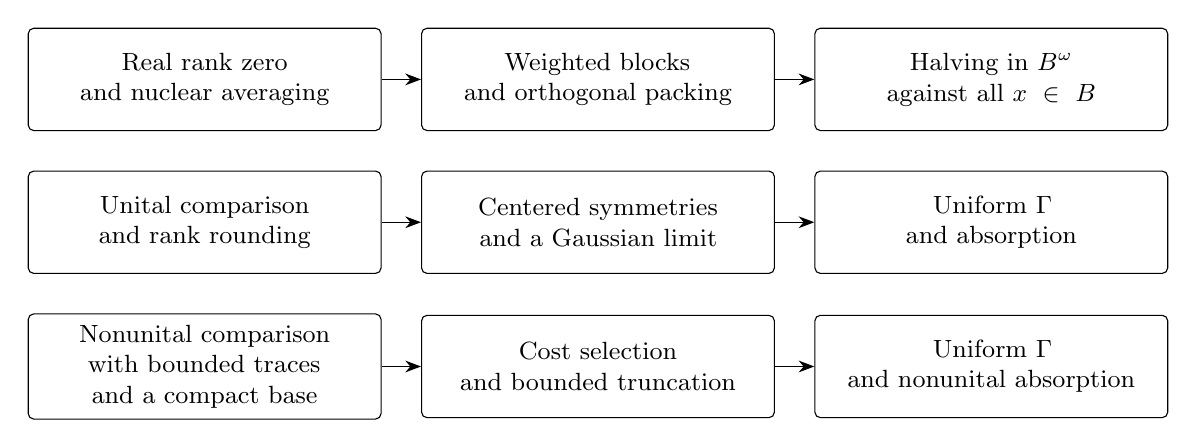
\begin{tikzpicture}[node distance=5mm and 5mm, every node/.style={font=\small},
 box/.style={draw,rounded corners=2pt,align=center,text width=42mm,
 minimum height=13mm,inner sep=4pt}, >={Stealth[length=2mm]}]
\node[box] (r1) {Real rank zero\\and nuclear averaging};
\node[box,right=of r1] (r2) {Weighted blocks\\and orthogonal packing};
\node[box,right=of r2] (r3) {Halving in $B^\omega$\\against all $x\in B$};
\node[box,below=of r1] (u1) {Unital comparison\\and rank rounding};
\node[box,right=of u1] (u2) {Centered symmetries\\and a Gaussian limit};
\node[box,right=of u2] (u3) {Uniform $\Gamma$\\and absorption};
\node[box,below=of u1] (n1) {Nonunital comparison\\with bounded traces\\and a compact base};
\node[box,right=of n1] (n2) {Cost selection\\and bounded truncation};
\node[box,right=of n2] (n3) {Uniform $\Gamma$\\and nonunital absorption};
\draw[->] (r1)--(r2); \draw[->] (r2)--(r3);
\draw[->] (u1)--(u2); \draw[->] (u2)--(u3);
\draw[->] (n1)--(n2); \draw[->] (n2)--(n3);
\end{tikzpicture}

\caption{Three routes to central coefficient-tested trace splitting. The
upper route uses real rank zero of the completion ultrapower. The lower
routes use comparison and supply their own projections in $A^\omega$.
Absorption is a consequence of the two comparison routes through the
published criteria verified in the text.}
\label{fig:routes}
\end{figure}

For the real-rank-zero route, Haagerup's convex virtual diagonal
\cite[Theorem~3.1]{Haa83} provides nuclear averaging maps chosen before
any input projection. Finite scalar compressions turn their outputs into
weighted matrix blocks. A small proportion of a base projection can be
sampled inside each block without making that subprojection central:
scalar matrix compressions retain the coefficient traces and squared
commutators. Orthogonal insertion then packs two labelled families with matching
target traces. The estimates use total weighted mass and energy, so they remain
independent of the number and sizes of the blocks. A bounded diagonal
argument yields the desired projection for the original ultrafilter, and
uniform $2$-density extends its identities from $A$ to its completion.

For the unital comparison route, a full positive element of small rank
receives an exact trace-preserving compression of a given positive element.
Integer spectral cuts approximate that trace by a finite-matrix rank, as
proved in Section~\ref{u:sec:ranks}; this elementary step needs neither
nuclearity nor comparison. Comparison then produces projections with exact
spectral support in $A^\omega$. Scalar compressions and matrix-unit transport
construct symmetries centered against any prescribed separable coefficient
algebra. The convex order-zero approximations of Hirshberg, Kirchberg and
White \cite[Theorem~1.4]{HKW} give a square-root-weighted sum of these
symmetries with fourth moment at most three. Its norm may grow with the
number of summands. Clipping at a fixed radius supplies bounded relative
moment estimates; successively adjoining commuting variables gives normalized sums with a
common Gaussian limit in coefficient traces. Continuous approximations to
equal-measure Gaussian intervals then yield the required central projections.

For the stably projectionless route, spectral allocation supplies small
projections with a one-sided cost bound. A single cost records both overlap
with earlier projections and error in a finite-dimensional model. A
block-matrix functional-calculus estimate passes aggregate squared
commutators to a truncated sum without a factor for the number of models.
The resulting small splittings have trace and projection errors of order
$\lambda^{3/2}$. Reindexing and multiplication amplify them to exact
splittings. The final passage distinguishes the uniform tracial ultrapower
$A^\omega$, the norm ultrapower $A_\omega$, and the annihilator quotient
$F_\omega(A)$, and checks generalized limit traces explicitly.

Sections~\ref{r:sec:preliminaries}--\ref{r:sec:completion} prove the
real-rank-zero route, including the finite-set theorem.
Sections~\ref{u:sec:preliminaries}--\ref{u:sec:gamma} give the direct unital
route and handle its empty-trace case. Sections~\ref{n:sec:framework}--
\ref{n:sec:absorption} give the bounded-trace nonunital route.
The elementary small-support lemma in Section~\ref{r:sec:projections}
serves both unital routes; Section~\ref{u:sec:ranks} proves the
trace-transfer and integer-rounding argument at its point of use.

\section{Notation and the tracial completion}\label{r:sec:preliminaries}

For a unital \(C^*\)-algebra \(D\), write \(\T(D)\) for its normalized tracial
states and \(\U(D)\) for its unitary group. For \(\tau\in\T(D)\), put
\[
 \normone{d}{\tau}=\tau(|d|),\qquad
 \normtwo{d}{\tau}=\tau(d^*d)^{1/2}.
\]
These may be seminorms. We use the finite von Neumann algebra obtained
from the tracial GNS representation when taking support projections,
polar decompositions, or signs in a trace calculation. In particular,
tracial Cauchy--Schwarz and trace-norm duality give
\begin{equation}\label{r:eq:trace-inequalities}
 \begin{aligned}
 |\tau(ab)|&\leq\normtwo{a}{\tau}\normtwo{b}{\tau},\qquad
 |\tau(ab)|\leq\norm a\normone b\tau,\\
 \norm{adb}_{s,\tau}&\leq\norm a\norm b\norm d_{s,\tau}
 \qquad(s=1,2).
 \end{aligned}
\end{equation}
In the last expression, \(\norm d_{s,\tau}\) denotes the corresponding
tracial seminorm. All uses of these inequalities also apply to the
unnormalized matrix trace \(\Tr\otimes\tau\). We always reserve \(\Tr\)
for the unnormalized scalar matrix trace. A scalar matrix over a corner
\(qDq\) is written \(G\otimes q\).

A projection is \emph{full} if the closed two-sided ideal it generates is
the whole algebra. For projections \(e,f\in D\), the notation
\(e\precsim f\) means that there is a partial isometry \(v\in D\) with
\(v^*v=e\) and \(vv^*\leq f\). Thus all projection comparisons used below
are implemented inside \(D\).
Real rank zero means that finite-spectrum self-adjoint elements are
norm dense in \(D_{\mathrm{sa}}\).

Every contraction in a unital \(C^*\)-algebra is a linear combination of four
unitaries whose coefficient absolute values sum to at most two. Indeed,
write \(a=h+ik\), where \(h,k\) are self-adjoint contractions, and use
\[
 h=\frac{u_h+u_h^*}{2},\qquad
 u_h=h+i(1-h^2)^{1/2},
\]
and the same formula for \(k\). Consequently, statements about a finite
set of elements can be reduced to statements about a finite set of
unitaries, with controlled constants.

\subsection{The specified completion and limit traces}

Let \(A\) be as in Theorem~\ref{r:thm:main}. For \(a\in A\), write
\[
 \normtwo a{\T(A)}
 =\sup_{\tau\in\T(A)}\tau(a^*a)^{1/2}.
\]
Let \(C\) be the \(C^*\)-algebra of operator-norm-bounded sequences in \(A\)
which are Cauchy for this norm, and let \(J\) consist of those sequences
whose uniform tracial 2-norm tends to zero. The uniform tracial
completion is \(B=C/J\), equipped with its quotient \(C^*\)-norm. The
designated traces on \(B\) are precisely
\[
 \bar\tau([(a_j)])=\lim_j\tau(a_j),\qquad \tau\in\T(A).
\]
These extensions define \(\normtwo{\cdot}{\T(A)}\) on \(B\).
No additional abstract traces of \(B\) enter this notation.

For a fixed free ultrafilter \(\omega\) on \(\N\), define
\begin{equation}\label{r:eq:ultrapower}
 B^\omega=\ell^\infty(\N,B)/I_\omega,\qquad
 I_\omega=\{(b_j):\lim_{j\to\omega}\normtwo{b_j}{\T(A)}=0\}.
\end{equation}
Here and below the sequences in \(I_\omega\) are operator-norm bounded.
For each sequence \((\tau_j)\) in \(\T(A)\), its \emph{limit trace} is
\begin{equation}\label{r:eq:limit-trace}
 \lambda([(b_j)])=\lim_{j\to\omega}\bar\tau_j(b_j).
\end{equation}
Write \(\Lambda_\omega\) for exactly this family of traces.

The copies of \(A\) and \(B\) given by constant sequences are faithful.
For \(A\), each trace is faithful by simplicity. For \(B\), uniform
2-Cauchyness shows that the functions
\(\tau\mapsto\tau(a_j^*a_j)\) converge uniformly. If all their limits
vanish, then \(\normtwo{a_j}{\T(A)}\to0\), so the class in \(B\) is zero.
The same observation identifies the constant copy of \(B\) in
\(B^\omega\).

We say that \(B\) has property \(\Gamma\), or equivalently that \(A\)
has \emph{uniform property \(\Gamma\)}, if there is a projection
\(p\in B^\omega\cap B'\) such that
\begin{equation}\label{r:eq:gamma-definition}
 \lambda(px)=\tfrac12\lambda(x)
 \quad(x\in B,\ \lambda\in\Lambda_\omega).
\end{equation}
This is the tracial-completion formulation of uniform property
\(\Gamma\); see \cite[Definition~16]{STW}. The relation with the standard
all-$m$ formulation uses the following interfaces. The framework of
\cite{CCEGSTW} takes the closed convex hull of \(\Lambda_\omega\) as its
designated ultrapower trace space. For fixed \(p,x\), the identity in
\eqref{r:eq:gamma-definition} extends to this closed convex hull by affine
weak-star continuity, and the supremum tracial 2-norm is unchanged.
The ultrapower identification and transfer
of relative commutants are given in \cite[Proposition~5.7]{CCEGSTW}, and
\cite[Proposition~5.20]{CCEGSTW} identifies uniform property $\Gamma$ of
$A$ with that of its completion. The passage from a halving projection to
equal coefficient-trace partitions is given by
\cite[Proposition~5.23 and Remark~5.24]{CCEGSTW}.
Our proof establishes \eqref{r:eq:gamma-definition} directly for the
specified completion and the originally fixed ultrafilter.

\section{Projection tools}\label{r:sec:projections}

Throughout this section, $D$ is a unital $C^*$-algebra of real rank zero
with $\T(D)\ne\varnothing$.  The trace estimates below hold simultaneously
for all $\tau\in\T(D)$.  The finite-set construction needs subprojections
with prescribed values on finitely many trace tests, followed by a way to
move them off previously occupied projections.  Scalar compressions and
proportional splitting provide the first step; the last lemma controls
the trace loss and displacement in the second.

\begin{lemma}[Scalar compressions]\label{r:proj:compress}
Every projection corner $rDr$ has real rank zero.  Moreover, given a
projection $r\in D$, a finite set $\mathcal F\subset D$, and $\gamma>0$,
there is a finite family of nonzero orthogonal projections $q_1,\ldots,q_m$
with sum $r$ such that
\begin{equation}\label{r:proj:compress-estimate}
  \dist(q_j hq_j,\C q_j)<\gamma
  \qquad(h\in\mathcal F,\ 1\le j\le m).
\end{equation}
The family is empty when $r=0$.
\end{lemma}

\begin{proof}
Let $r\ne0$ and $h=h^*\in rDr$.  Choose $R>\norm{h}+2$ and finite-spectrum
self-adjoints $a_n\in D$ converging in norm to $h+Rr$.  The spectrum of the
limit is contained in $\{0\}\cup(2,\infty)$, so the spectral projections
$f_n=1_{(1,\infty)}(a_n)$ converge in norm to $r$.  For all sufficiently
large $n$, the element
\[
  r f_n+(1-r)(1-f_n)
\]
is invertible.  Its unitary polar part $u_n$ satisfies
$u_n f_n u_n^*=r$ and $u_n\to1$ in norm.  Since $a_n$ commutes with $f_n$,
the compression $r u_n a_n u_n^*r$ has finite spectrum in $rDr$.
Subtracting $Rr$ gives finite-spectrum approximations to $h$ in that
corner.

For the second assertion, first replace $\mathcal F$ by its real and
imaginary parts.  Compress the first self-adjoint test to $rDr$, approximate
it by a finite-spectrum self-adjoint, and partition $r$ by the latter's
spectral projections.  Repeat for each subsequent test in every current
corner.  An estimate
$\norm{q hq-\lambda q}<\delta$ persists on every subprojection of $q$.
Thus this finite refinement procedure preserves all earlier estimates.
Using tolerance less than $\gamma/2$ for the real and imaginary parts
proves \eqref{r:proj:compress-estimate}; zero pieces are discarded.
\end{proof}

The next fact concerns a simple unital algebra alone. It uses neither
real rank zero nor nuclearity nor comparison, and will also supply the
small hereditary support for the rank approximation in
Section~\ref{u:sec:ranks}.

\begin{lemma}[Full positive elements with small tracial support]
\label{u:lem:thin-full}
Let $A$ be simple, unital and infinite dimensional, with
$T(A)\ne\varnothing$.  For every $\delta>0$ there is a full positive element
$e\in A$ with $\norm e=1$ such that
\[
 \tau(\supp(e))<\delta\qquad(\tau\in T(A)).
\]
Here supports and traces are taken in each tracial von Neumann representation.
\end{lemma}

\begin{proof}
First we obtain arbitrarily many mutually orthogonal nonzero positive
elements.  Choose a maximal abelian unital $C^*$-subalgebra $E\subset A$.
Suppose that $E$ were finite dimensional, with minimal projections
$p_1,\ldots,p_m$ summing to $1$.  Every selfadjoint element of $p_iAp_i$
commutes with $E$, so maximality implies $p_iAp_i=\C p_i$.  If
$0\ne x\in p_iAp_j$, then
\[
 x^*x=\norm{x}^2p_j,\qquad xx^*=\norm{x}^2p_i.
\]
Thus $u=x/\norm{x}$ satisfies $u^*u=p_j$ and $uu^*=p_i$.  For any
$y\in p_iAp_j$, the element $u^*y$ is scalar on $p_j$, and
$y=u(u^*y)$.  Consequently each $p_iAp_j$ has dimension at most one.
The decomposition $A=\sum_{i,j}p_iAp_j$ would make $A$ finite
dimensional, a contradiction.  Hence $E\cong C(X)$ for an infinite
compact Hausdorff space $X$.  Given $k\in\N$, choose $k$ distinct points
of $X$, pairwise disjoint neighborhoods, and nonzero positive continuous
functions supported in those neighborhoods.  Their images give mutually
orthogonal nonzero positive elements $c_1,\ldots,c_k\in A$.

For two nonzero positive elements $c,d\in A$, simplicity gives $cAd\ne0$.
Indeed, if $cAd=0$, then $c$ annihilates the ideal generated by $d$;
this ideal is $A$, which would force $c=0$.  Choose $y\in A$ such that
$z=cyd\ne0$.  Then $z^*z\in\overline{dAd}$ and $zz^*\in\overline{cAc}$.
In each tracial von Neumann representation, the polar decomposition of
$z$ gives a partial isometry with
initial projection $\supp(z^*z)$ and final projection $\supp(zz^*)$.
The normal tracial state therefore gives
\[
 \tau(\supp(z^*z))=\tau(\supp(zz^*))
 \le \min\{\tau(\supp(c)),\tau(\supp(d))\}
 \qquad(\tau\in T(A)).
\]
The elements $y,z$ are chosen independently of $\tau$; the support
comparison holds in every tracial representation.
Start with $c=c_1$. For $j=2,\ldots,k$, apply the preceding construction
with $d=c_j$ and replace $c$ by $zz^*$. The support trace never increases
and is at most the support trace of $c_j$. The final nonzero positive
element $e=c$ therefore has support trace at most that of each $c_i$,
at every trace.  Since the support
projections of the $c_i$ are orthogonal,
\[
 k\,\tau(\supp(e))\le\sum_{i=1}^k\tau(\supp(c_i))\le1
 \qquad(\tau\in T(A)).
\]
Choose $k$ with $1/k<\delta$ and rescale $e$ to have norm one, which
does not change its support.  It is full because $A$ is simple.
\end{proof}

We return to the ambient algebra $D$. Real rank zero will produce a
projection by a spectral cut; the norm-one normalization will let us prove
that this projection is full by testing proper quotients of $D$.

\begin{lemma}[Small full projections]\label{r:proj:small}
Suppose that $D$ contains a unital simple infinite-dimensional
$C^*$-subalgebra $A$.  For every $\delta>0$, there is a full projection
$g\in D$ such that
\[
  \sup_{\tau\in\T(D)}\tau(g)<\delta.
\]
\end{lemma}

\begin{proof}
The restriction to $A$ of any trace in $\T(D)$ is a tracial state,
so $\T(A)\ne\varnothing$. Given a positive integer $n$, apply
Lemma~\ref{u:lem:thin-full} to obtain $b\in A_+$ with $\norm b=1$ and
\begin{equation}\label{r:proj:small-positive}
 \rho(b)\le\rho(\supp(b))<\frac1n
 \qquad(\rho\in\T(A)).
\end{equation}

Choose a finite-spectrum self-adjoint $a\in D$ with
$\norm{a-b}<1/8$, and set $g=1_{[1/2,\infty)}(a)$.  Then
$gbg\ge(3/8)g$, so restriction of any $\tau\in\T(D)$ to $A$ gives
\begin{equation}\label{r:proj:small-projection-bound}
  \tau(g)\le\frac83\tau(b)\le\frac{8}{3n}.
\end{equation}
We claim that $g$ is full in $D$.  Otherwise, let $\pi:D\to D/I$ be the quotient
by the proper closed ideal generated by $g$.  The inequalities
$a\ge-1/8$ and $a(1-g)\le(1/2)(1-g)$ imply
$\norm{\pi(a)}\le1/2$, and hence $\norm{\pi(b)}\le5/8$.
On the other hand, $\pi|_A$ is a unital homomorphism from the simple
algebra $A$ to a nonzero unital algebra.  It is injective and therefore
isometric, contradicting $\norm{b}=1$.  Thus $g$ is full, and choosing
$n$ with $8/(3n)<\delta$ finishes the proof.
\end{proof}

We will use an elementary splitting procedure with different target
projections.  Zero projections are allowed among the resulting pieces.

\begin{lemma}[Splitting a column]\label{r:proj:columns}
Let $f,g_1,\ldots,g_m$ be projections in $D$, where $m\ge1$.
Suppose that $v_1,\ldots,v_m\in D$ satisfy
\[
  v_i=g_i v_i f,
  \qquad \sum_{i=1}^m v_i^*v_i=f.
\]
There are orthogonal projections $e_1,\ldots,e_m$ with sum $f$ and
$e_i\precsim g_i$ for every $i$.
\end{lemma}

\begin{proof}
If $f=0$, take all $e_i=0$.  We argue by induction on $m$; for $m=1$,
$v_1$ itself implements $f\precsim g_1$.  Suppose that $m>1$.
Apply Lemma~\ref{r:proj:compress} to choose a finite-spectrum self-adjoint
$a\in fDf$ within $1/8$ of $v_1^*v_1$.  Set
\[
  e_1=1_{[1/2,\infty)}(a),\qquad r=f-e_1.
\]
The inequality $e_1v_1^*v_1e_1\ge(3/8)e_1$ shows that, when $e_1\ne0$,
\[
  v_1e_1(e_1v_1^*v_1e_1)^{-1/2}
\]
is a partial isometry with initial projection $e_1$ and final projection
below $g_1$.  On the remaining corner,
\[
  Q:=\sum_{i=2}^m r v_i^*v_i r
    =r-rv_1^*v_1r\ge\frac38r.
\]
If $r=0$, take $e_2=\cdots=e_m=0$.  Otherwise define
$w_i=v_i r Q^{-1/2}$ for $i=2,\ldots,m$, with the inverse taken in $rDr$.
These elements satisfy $w_i=g_iw_i r$ and
$\sum_{i=2}^m w_i^*w_i=r$.  The induction hypothesis partitions $r$ as
required.
\end{proof}

Approximate projection halving in non-elementary simple real-rank-zero
algebras was developed by Zhang \cite[Theorem~1.1(i)]{Zhang1991}.
More directly, Zhang's ordered-decomposition lemma
\cite[Lemma~1.1]{Zhang1990}, as used in Vaccaro's divisibility
argument~\cite[Lemma~2.1, version~1]{Vac26}, applies without
simplicity: a projection can be
partitioned into finitely many pieces ordered by subequivalence and each
subequivalent to any given full projection. We give this projection
construction below and then use a common rounding rule to obtain
proportional trace splitting uniformly over all traces.

\begin{proposition}[Uniform proportional subprojections]\label{r:proj:split}
Assume that for every $\delta>0$ there is a full projection $g\in D$ with
$\sup_{\tau\in\T(D)}\tau(g)<\delta$.
For every projection $f\in D$, every $s\in[0,1]$, and every $\eps>0$,
there is a projection $e\le f$ such that
\begin{equation}\label{r:proj:split-estimate}
  \sup_{\tau\in\T(D)}|\tau(e)-s\tau(f)|<\eps.
\end{equation}
\end{proposition}

\begin{proof}
The case $f=0$ is immediate.  Choose a full projection $g$ with
$\sup_\tau\tau(g)<\eps$.  Fullness provides a finite sum
$\sum_i x_i g y_i$ within distance less than one of $1$.
Write $X=[x_1\ \cdots\ x_m]$ and let $Y$ be the column with entries
$gy_i$.  Then $XY$ is invertible, so $Y$ has a bounded left inverse
$L=(XY)^{-1}X$.  In particular,
\[
  1=Y^*L^*LY\le\norm{L}^2Y^*Y,
\]
and $Y^*Y$ is invertible.  The entries of
$Y(Y^*Y)^{-1/2}f$ form a column as in Lemma~\ref{r:proj:columns}, with every
target projection equal to $g$.  We obtain an orthogonal family with
sum $f$, each member subequivalent to $g$.

We next replace this family by one, say $s_1,\ldots,s_m$, satisfying
\begin{equation}\label{r:proj:ordered-partition}
  s_1\precsim s_2\precsim\cdots\precsim s_m\precsim g.
\end{equation}
This ordering makes the trace weights increase in the same order for
every trace, so that one choice of rounding coefficients will work
simultaneously for all of them.
Here is the pair operation that makes this possible.  Suppose that $x,y$
are orthogonal pieces, both subequivalent to a common projection $h$.
Choose partial isometries $w,u$ with
\[
  w^*w=x,\quad ww^*=x'\le h,
  \qquad u^*u=y,\quad uu^*\le h.
\]
Since $u^*x'u+u^*(h-x')u=y$, Lemma~\ref{r:proj:columns} applied to the
column with entries $x'u,(h-x')u$ gives $y=k+l$ and partial isometries
$\alpha,\beta$ with
\[
  \alpha^*\alpha=k,\quad \alpha\alpha^*\le x',
  \qquad \beta^*\beta=l,\quad \beta\beta^*\le h-x'.
\]
Set $\xi=w^*\alpha+l$ and $\zeta=w+\beta$.  Then
\begin{align*}
  \xi^*\xi&=y,&
  \xi\xi^*&=w^*\alpha\alpha^*w+l\le x+l,\\
  \zeta^*\zeta&=x+l,&
  \zeta\zeta^*&=x'+\beta\beta^*\le h.
\end{align*}
The cross terms vanish by orthogonality of the initial and final
components: $x\perp l$ and $x'\perp(h-x')$.
Thus replacing $x,y$ by $k,x+l$
preserves their sum and orthogonality, and
\[
  k\precsim x\le x+l,
  \qquad x,y\precsim x+l\precsim h.
\]
After each adjacent comparison, the new right-hand piece dominates
every piece already passed: it contains the previous moving piece.
Thus a left-to-right pass with common bound $g$ leaves a last piece
dominating all earlier pieces.  Freeze that last
piece and repeat on the shorter list, now using it as the common bound.
Induction gives \eqref{r:proj:ordered-partition}.  All operations take place
inside $D$ and preserve the orthogonal sum $f$.

Set
\[
  c_i=\lfloor si\rfloor-\lfloor s(i-1)\rfloor\in\{0,1\},
  \qquad e=\sum_{i=1}^m c_i s_i.
\]
For a fixed $\tau\in\T(D)$, put $t_i=\tau(s_i)$ and
$D_j=\lfloor sj\rfloor-sj$.  Then $t_1\le\cdots\le t_m\le\tau(g)$ and
$-1\le D_j\le0$.  Summation by parts gives
\[
  \tau(e)-s\tau(f)
   =D_m t_m+\sum_{i=1}^{m-1}D_i(t_i-t_{i+1}).
\]
The first term lies in $[-t_m,0]$, while the sum lies in
$[0,t_m-t_1]$.  It follows that
$|\tau(e)-s\tau(f)|\le t_m\le\tau(g)$, proving
\eqref{r:proj:split-estimate} uniformly in $\tau$.
\end{proof}

\begin{corollary}[Splitting finite linear tests]\label{r:proj:tests}
Under the small-full-projection hypothesis of Proposition~\ref{r:proj:split},
let $q\in D$ be a projection, $s\in[0,1]$, and $\mathcal F\subset D$ a
finite set.  For every $\eps>0$, there is a projection $e\le q$ such that
\begin{equation}\label{r:proj:tests-estimate}
  |\tau(eh)-s\tau(qh)|<\eps
  \qquad(h\in\mathcal F,\ \tau\in\T(D)).
\end{equation}
\end{corollary}

\begin{proof}
The assertion is immediate if $q=0$ or $\mathcal F$ is empty.  Choose
$\gamma>0$ with $2\gamma<\eps/2$ and use
Lemma~\ref{r:proj:compress} to write $q=\sum_{j=1}^m q_j$ with
\[
  \norm{q_j hq_j-\lambda_{j,h}q_j}<\gamma
  \qquad(h\in\mathcal F)
\]
for suitable scalars $\lambda_{j,h}$.  These scalars satisfy
$|\lambda_{j,h}|\le\norm{h}+\gamma$.
Put $M=\max_{h\in\mathcal F}\norm{h}+\gamma$ and choose
$\delta>0$ with $mM\delta<\eps/2$.
By Proposition~\ref{r:proj:split}, choose $e_j\le q_j$ so that
$|\tau(e_j)-s\tau(q_j)|<\delta$ for every $\tau$, and set
$e=\sum_j e_j$.  Traciality removes all off-diagonal compressions and gives
\begin{align*}
  |\tau(eh)-s\tau(qh)|
  &\le \gamma\bigl(\tau(e)+s\tau(q)\bigr)
       +\sum_{j=1}^m |\lambda_{j,h}|
          |\tau(e_j)-s\tau(q_j)| \\
  &\le 2\gamma+mM\delta<\eps.
\end{align*}
\end{proof}

The last tool moves a projection off an occupied corner.  Its linear
trace estimate retains the scale of the projection being moved.

\begin{lemma}[Orthogonal insertion]\label{r:proj:move}
For projections $z,y\in D$, there is a projection $t\le1-z$ such that
\begin{align}
  \tau(y)-3\tau(yz)&\le\tau(t)\le\tau(y),
       \label{r:proj:move-mass}\\
  \normtwo{t-y}{\tau}^{2}&\le5\tau(yz)
       \label{r:proj:move-distance}
\end{align}
for every $\tau\in\T(D)$.  For every contraction $x\in D$, it also
satisfies
\begin{equation}\label{r:proj:move-linear}
  |\tau((t-y)x)|
   \le2\sqrt{\tau(y)}\,\normtwo{t-y}{\tau}.
\end{equation}
\end{lemma}

\begin{proof}
If $y=0$, take $t=0$.  Otherwise choose, in $yDy$, a finite-spectrum
self-adjoint $a$ with $\norm{a-yzy}<1/8$, and let
$f=1_{(-\infty,1/2)}(a)$.  Writing $d=y-f$, we have
\[
  d(yzy)d\ge\frac38d,
  \qquad f(yzy)f\le\frac58f.
\]
Since $yzy\ge0$, this implies
\begin{equation}\label{r:proj:discarded-mass}
  \tau(y-f)\le\frac83\tau(yz),
  \qquad A_f:=f(1-z)f\ge\frac38f.
\end{equation}
If $f=0$, put $t=0$.  Otherwise the element
\[
  v=(1-z)f A_f^{-1/2}
\]
is a partial isometry with $v^*v=f$; set $t=vv^*\le1-z$.
In both cases,
\[
  \tau(t)=\tau(f),\qquad ftf=f(1-z)f.
\]
The mass bounds \eqref{r:proj:move-mass} follow from
\eqref{r:proj:discarded-mass}.  As $f\le y$,
\[
  \tau(ty)\ge\tau(tf)=\tau(f)-\tau(fz).
\]
Consequently,
\begin{align*}
  \normtwo{t-y}{\tau}^{2}
   &=\tau(t)+\tau(y)-2\tau(ty)\\
   &\le\tau(y-f)+2\tau(fz)
    \le\left(\frac83+2\right)\tau(yz)
    \le5\tau(yz),
\end{align*}
which proves \eqref{r:proj:move-distance}.

Finally, decompose $t-y=t(t-y)+(1-t)(t-y)$.  The first summand has left
support below $t$, and the second equals $-(1-t)y$ and has right support
below $y$.  Tracial Cauchy--Schwarz therefore gives
\[
  \normone{t-y}{\tau}
   \le\bigl(\sqrt{\tau(t)}+\sqrt{\tau(y)}\bigr)
       \normtwo{t-y}{\tau}
   \le2\sqrt{\tau(y)}\,\normtwo{t-y}{\tau}.
\]
Trace-norm duality proves \eqref{r:proj:move-linear}.
\end{proof}

\section{Nuclear averaging and weighted matrix blocks}\label{r:sec:weighted}

In this section \(A\subseteq D\) is a unital inclusion, \(A\) is nuclear,
and \(D\) has real rank zero and nonempty tracial state space. For a
prescribed finite set of unitary tests, nuclear averaging turns a
projection into a nearly central positive contraction. We will approximate
this contraction in trace by a weighted sum of projections, keeping their
total weighted squared commutator norm small. Each projection will also
be represented as a matrix block over a projection \(q\), with each
compressed test close to a scalar matrix over \(q\). This lets us sample
a subprojection \(e\leq q\) simultaneously in the matrix coordinates
while retaining trace and commutator estimates, without requiring \(e\)
to be central. We first choose the averaging map, independently of its
input projection.

\begin{lemma}[Averaging with trace control]\label{r:weighted:diagonal}
For a finite \(K\subseteq\U(A)\) and \(\mu>0\), there are contractions
\(v_1,\ldots,v_m\in A\) and numbers \(\lambda_l\geq0\) with
\(\sum_l\lambda_l=1\) such that the map
\[
 \Phi(b)=\sum_{l=1}^m\lambda_l v_lbv_l^*,\qquad b\in D,
\]
satisfies, for every projection \(q\in D\), every \(x\in K\), and every
\(\tau\in\T(D)\),
\begin{align}
 0\leq\Phi(q)&\leq1,\qquad
 \tau(q)-\mu\leq\tau(\Phi(q))\leq\tau(q),\label{r:eq:diagonal-mass}\\
 \normone{\Phi(q)-x\Phi(q)x^*}{\tau}
 &\leq\mu\tau(q).\label{r:eq:diagonal-central}
\end{align}
\end{lemma}

\begin{proof}
Let \(E=A\widehat\otimes A\) denote the Banach projective tensor product,
with norm \(\norm{\cdot}_\pi\), multiplication map
\(m_A(a\otimes b)=ab\), and bimodule actions
\(x\cdot(a\otimes b)=xa\otimes b\) and
\((a\otimes b)\cdot x=a\otimes bx\).
Haagerup's virtual diagonal theorem
\cite[Theorem~3.1]{Haa83} gives a virtual diagonal \(M\in E^{**}\) in
the weak-star closed convex hull of
\(\{v\otimes v^*:v\in A,\ \norm v\leq1\}\).
Its bimodule commutators vanish and \(m_A^{**}(M)=1\).
Apply the second adjoint of the bounded linear map
\[
 T:E\longrightarrow E^K\oplus A,\qquad
 T(d)=\big((x\cdot d-d\cdot x)_{x\in K},m_A(d)\big).
\]
Its value at \(M\) is \((0,\ldots,0,1)\), in the canonical copy of
\(E^K\oplus A\). Weak-star convergence in the bidual restricts to weak
convergence in this copy, so this point lies in the weak closure of the
image of the finite convex hull. A convex subset of a Banach space has the
same weak and norm closures, by Hahn--Banach separation. We may therefore choose a finite
convex combination \(d=\sum_l\lambda_l v_l\otimes v_l^*\) such that
\begin{equation}\label{r:eq:approx-diagonal}
 \norm{x\cdot d-d\cdot x}_\pi<\mu\quad(x\in K),\qquad
 \norm{1-\sum_l\lambda_l v_lv_l^*}<\mu.
\end{equation}

Both sums \(\sum_l\lambda_l v_lv_l^*\) and
\(\sum_l\lambda_l v_l^*v_l\) are positive contractions. By traciality,
the positive element \(c=1-\sum_l\lambda_l v_l^*v_l\) satisfies
\(0\leq\tau(c)<\mu\). Since
\(\tau(q)-\tau(\Phi(q))=\tau(qc)\), this proves
\eqref{r:eq:diagonal-mass}.
For the centrality estimate, the map
\(a\otimes b\mapsto aqb\) has norm at most \(\tau(q)\) from the
projective tensor norm to the tracial 1-seminorm: indeed,
\[
 \normone{aqb}{\tau}
 \leq\normtwo{aq}{\tau}\normtwo{qb}{\tau}
 \leq\norm a\norm b\,\tau(q).
\]
Apply this map to the first inequality in \eqref{r:eq:approx-diagonal}
and multiply by the unitary \(x^*\).
\end{proof}

The following tracial square-root estimate is the form of the
Powers--St\o rmer inequality needed below. Their original
\cite[Lemma~4.1]{PowersStormer1970} concerns positive Hilbert-space
operators with the ordinary trace; the short proof here gives the
arbitrary tracial $C^*$-algebra version directly.

\begin{lemma}[A square-root trace estimate]\label{r:weighted:square-root}
For positive \(b,c\in D\) and \(\tau\in\T(D)\),
\[
 \normtwo{\sqrt b-\sqrt c}{\tau}^2
 \leq\normone{b-c}{\tau}.
\]
\end{lemma}

\begin{proof}
Work in the tracial von Neumann algebra and put \(d=\sqrt b-\sqrt c\).
Traciality and \(b-c=\sqrt b\,d+d\sqrt c\) give
\[
 \tau(\sgn(d)(b-c))=\tau((\sqrt b+\sqrt c)|d|).
\]
Since \(\sqrt b+\sqrt c\geq d\) and
\(\sqrt b+\sqrt c\geq-d\), tracing against the positive and negative
parts \(d_+\) and \(d_-\), respectively, bounds the right-hand side
below by \(\tau(d_+^2)+\tau(d_-^2)=\tau(d^2)\).
Trace-norm duality bounds the left-hand side by
\(\normone{b-c}{\tau}\).
\end{proof}

\begin{proposition}[Weighted matrix blocks]\label{r:weighted:family}
Let \(K\subseteq\U(A)\) be finite and \(0<\eta<1\).
There are contractions \(v_1,\ldots,v_m\in A\) and nonnegative numbers
\(\lambda_1,\ldots,\lambda_m\) summing to one, chosen using only
\(K,\eta\), such that the map
\begin{equation}\label{r:eq:averaging-map}
 \Phi:D\longrightarrow D,\qquad
 \Phi(b)=\sum_{l=1}^m\lambda_l v_lbv_l^*,
\end{equation}
satisfies \eqref{r:eq:diagonal-mass} with \(\mu=\eta^2\).
For every projection \(r\in D\), there is a finite family consisting of
weights \(0<w_j\leq1\), nonzero projections \(q_j\leq r\), integers
\(k_j\geq1\), and rows \(U_j\in M_{1,k_j}(D)\), such that, with
\(p_j=U_jU_j^*\),
\begin{align}
 U_j^*U_j&=1_{k_j}\otimes q_j,\label{r:eq:block-isometry}\\
 \dist\big(U_j^*xU_j,M_{k_j}(\C)\otimes q_j\big)&<\eta
       &&(x\in K),\label{r:eq:block-compression}\\
 \normone{\sum_jw_jp_j-\Phi(r)}{\tau}&\leq\eta^2,
       \label{r:eq:block-mass}\\
 \sum_jw_j\normtwo{[x,p_j]}{\tau}^2&\leq6\eta
       &&(x\in K).\label{r:eq:block-energy}
\end{align}
The last two estimates hold for every \(\tau\in\T(D)\). The family may
be empty; the base projections \(q_j\) may repeat, and the projections
\(p_j\) need not be mutually orthogonal.
\end{proposition}

\begin{proof}
Put \(\mu=\eta^2\) and choose \(\Phi\) by
Lemma~\ref{r:weighted:diagonal}. In particular, the coefficient list is
fixed before \(r\). Choose \(0<\sigma<1\), then \(\beta>0\), so that
\begin{equation}\label{r:eq:block-parameters}
 \beta<\sigma/2,\qquad m(\sigma+2\beta)<\mu,\qquad
 \frac{2\beta}{\sigma}
       +\frac{(2+\sqrt2)\beta}{\sigma^2}<\eta.
\end{equation}
This is possible by choosing \(\sigma\) with \(m\sigma<\mu\) first.

\paragraph{Scalar matrix approximation.}
Partition \(r\) by Lemma~\ref{r:proj:compress}, using the finite list
\[
 v_l^*v_n,\quad v_l^*xv_n
 \qquad(1\leq l,n\leq m,\ x\in K).
\]
Take the compression tolerance smaller than \(\beta/(2m)\).
For a nonzero partition piece \(q\), set
\[
 V=[\sqrt{\lambda_l}\,v_lq]_{l=1}^m,\quad
 h_q=VV^*=\Phi(q),\quad M=V^*V,\quad N_x=V^*xV.
\]
These are contractions in their respective matrix spaces.
Apply any state of \(qDq\) entrywise to \(M,N_x\), obtaining scalar
matrices \(G,H_x\). Positivity and contractivity of a state at matrix
levels give \(0\leq G\leq1\) and \(\norm{H_x}\leq1\).
The compression tolerance implies
\begin{equation}\label{r:eq:scalar-gram}
 \norm{M-G\otimes q}<\beta,\qquad
 \norm{N_x-H_x\otimes q}<\beta.
\end{equation}
Indeed, each unweighted entry differs from its scalar state value by
less than twice the compression tolerance, and an \(m\)-by-\(m\) matrix
of entries of norm at most \(c\) has norm at most \(mc\).

\paragraph{Construction of the blocks.}
Rotate the columns of \(V\) by a scalar unitary diagonalizing \(G\).
Retain the columns corresponding to eigenvalues at least \(\sigma\),
forming a row \(W\) with \(k\) columns and scalar diagonal matrix \(G_+\).
The cutoff gives the uniform lower bound needed to normalize the retained
row by an inverse square root.
If \(k=0\), set \(b_q=0\). Otherwise put
\begin{equation}\label{r:eq:polar-block}
 X=W^*W\geq(\sigma/2)(1_k\otimes q),\qquad
 U=WX^{-1/2},\qquad b_q=U(G_+\otimes q)U^*.
\end{equation}
Then \(U^*U=1_k\otimes q\), so \(b_q\) is a finite-spectrum positive
contraction.
Writing \(W_-\) for the row of deleted columns, we have
\(\norm{W_-^*W_-}\leq\sigma+\beta\), and therefore
\[
 \tau(W_-W_-^*)=(\Tr\otimes\tau)(W_-^*W_-)
 \leq m(\sigma+\beta)\tau(q).
\]
The contribution is zero if no columns are deleted. Also
\[
 b_q-WW^*=U(G_+\otimes q-X)U^*
\]
has norm at most \(\beta\), supported on a projection of trace
\(k\tau(q)\). Consequently, including the case \(k=0\),
\begin{equation}\label{r:eq:finite-spectrum-close}
 \normone{b_q-h_q}{\tau}
 \leq m(\sigma+2\beta)\tau(q)\leq\mu\tau(q).
\end{equation}

We verify explicitly that the compression estimate is independent of
the corner and its matrix size. For positive invertible \(X,Y\geq a1\),
the resolvent formula for inverse square roots gives
\begin{equation}\label{r:eq:inverse-root}
 \norm{X^{-1/2}-Y^{-1/2}}
 \leq\frac{\norm{X-Y}}{\pi}
       \int_0^\infty\frac{t^{-1/2}}{(a+t)^2}\,dt
 =\frac{\norm{X-Y}}{2a^{3/2}}.
\end{equation}
Use \(Y=G_+\otimes q\) and \(a=\sigma/2\).
If \(H\otimes q\) denotes the corresponding retained corner of
\(H_x\otimes q\), then \(\norm H\leq1\), and
\eqref{r:eq:scalar-gram} gives
\(\norm{W^*xW-H\otimes q}<\beta\).
Expanding the difference between
\[
 U^*xU=X^{-1/2}(W^*xW)X^{-1/2}
 \quad\hbox{and}\quad Y^{-1/2}(H\otimes q)Y^{-1/2}
\]
and using \eqref{r:eq:inverse-root} bounds its norm by
\[
 \frac{2\beta}{\sigma}
 +\frac{(2+\sqrt2)\beta}{\sigma^2}<\eta.
\]
The second expression is a scalar matrix over \(q\). The tolerances
\(\sigma,\beta\) were chosen before the partition of \(r\), so the
compression bound is uniform over its pieces.

Write \(b_q\) as the finite sum of its nonzero upper spectral
projections, weighted by the lengths of their level intervals:
\begin{equation}\label{r:eq:layer-cake}
 b_q=\int_0^1 1_{(a,\infty)}(b_q)\,da
     =\sum_{j\in J_q}w_jp_j.
\end{equation}
Each \(p_j\) is the image of a scalar coordinate projection under \(U\).
It therefore has a subrow \(U_j\) satisfying
\eqref{r:eq:block-isometry}, with \(q_j=q\).
Taking matrix corners gives \eqref{r:eq:block-compression}.
Summing \eqref{r:eq:finite-spectrum-close} over the partition gives
\eqref{r:eq:block-mass}.

\paragraph{Averaged commutators.}
For a finite-spectrum
positive contraction \(b=\sum_s s e_s\), include its kernel projection
in this spectral resolution. Tracial orthogonality gives, for unitary
\(x\),
\begin{align}
 \int_0^1\normtwo{[x,1_{(a,\infty)}(b)]}{\tau}^2\,da
 &=\sum_{s,t}|s-t|\normtwo{e_sxe_t}{\tau}^2\notag\\
 &\leq2\sqrt{\tau(b)}\,\normtwo{[x,\sqrt b]}{\tau}\notag\\
 &\leq2\sqrt{\tau(b)\normone{b-xbx^*}{\tau}}.
 \label{r:eq:spectral-energy}
\end{align}
For the middle inequality, factor
\(|s-t|=|\sqrt s-\sqrt t|(\sqrt s+\sqrt t)\) and apply
Cauchy--Schwarz to the sum. The second squared sum is at most
\(2\sum_{s,t}(s+t)\normtwo{e_sxe_t}{\tau}^2=4\tau(b)\).
The last inequality is Lemma~\ref{r:weighted:square-root}.

For \(b=b_q\), equations \eqref{r:eq:diagonal-mass},
\eqref{r:eq:diagonal-central}, and \eqref{r:eq:finite-spectrum-close} give
\[
 \tau(b_q)\leq(1+\mu)\tau(q),\qquad
 \normone{b_q-xb_qx^*}{\tau}\leq3\mu\tau(q).
\]
Thus the contribution of \(J_q\) in \eqref{r:eq:block-energy} is at most
\(2\sqrt{3(1+\mu)}\,\eta\tau(q)\leq6\eta\tau(q)\).
Summing over \(q\) proves the assertion.
\end{proof}

\section{Sampling and orthogonal packing}\label{r:sec:packing}

Continue with the inclusion \(A\subseteq D\) from
Section~\ref{r:sec:weighted}. The matrix compressions from
Proposition~\ref{r:weighted:family} allow
us to sample a projection without making the sampled corner central.
We isolate the precise estimate before carrying out the packing.

\begin{lemma}[Sampling a matrix block]\label{r:packing:sampling}
Let \(q\in D\) be a nonzero projection and let \(U\in M_{1,k}(D)\)
satisfy \(U^*U=1_k\otimes q\). Put \(p=UU^*\).
Suppose \(x\in\U(D)\), \(0<\eta<1\), and
\[
 \dist(U^*xU,M_k(\C)\otimes q)<\eta.
\]
For a projection \(e\leq q\), set \(y=U(1_k\otimes e)U^*\).
Then, for \(0\leq c\leq1\), every \(\tau\in\T(D)\), and
\(\delta_\tau=|\tau(y)-c\tau(p)|\),
\begin{align}
 |\tau(yx)-c\tau(px)|
 &\leq\eta\big(\tau(y)+c\tau(p)\big)+2\delta_\tau,
 \label{r:eq:sampling-linear}\\
 \left|\normtwo{[x,y]}{\tau}^2
        -c\normtwo{[x,p]}{\tau}^2\right|
 &\leq6\eta\big(\tau(y)+c\tau(p)\big)+10\delta_\tau.
 \label{r:eq:sampling-energy}
\end{align}
\end{lemma}

\begin{proof}
Write \(T=U^*xU\), \(P_e=1_k\otimes e\), and choose \(T_0\in M_k(\C)\)
with \(\norm{T-T_0\otimes q}<\eta\).
Since \(T\) is a contraction, \(\norm{T_0}\leq2\).
The map \(a\mapsto UaU^*\) identifies the relevant matrix corner with
its image in \(D\), and therefore
\[
 \tau(yx)=(\Tr\otimes\tau)(P_eTP_e),\qquad
 \tau(|yxy|^2)=(\Tr\otimes\tau)(|P_eTP_e|^2).
\]
The scalar matrix \(T_0\otimes q\) commutes with \(P_e\), whether or not
\(e\) commutes with any entry of \(T\).
Thus replacing \(P_eTP_e\) by \(T_0\otimes e\) changes these two traces
by at most \(\eta\tau(y)\) and \(3\eta\tau(y)\), respectively.
For the latter estimate use
\[
 \norm{R^*R-S^*S}\leq(\norm R+\norm S)\norm{R-S},
 \quad R=P_eTP_e,\quad S=T_0\otimes e,
\]
and the fact that the trace of the corner unit is
\((\Tr\otimes\tau)(P_e)=k\tau(e)=\tau(y)\).
The same estimates hold with \(e\) replaced by \(q\).

Set
\[
 \alpha=\frac{\Tr(T_0)}{k},\qquad
 \beta_0=\frac{\Tr(T_0^*T_0)}{k}.
\]
Then \(|\alpha|\leq2\) and \(0\leq\beta_0\leq4\).
The scalar reference traces for \(y\) are
\(\alpha\tau(y)\) and \(\beta_0\tau(y)\); for \(p\), they are
\(\alpha\tau(p)\) and \(\beta_0\tau(p)\).
This proves \eqref{r:eq:sampling-linear}.
For the second estimate, the exact identity
\begin{equation}\label{r:eq:unitary-energy}
 \normtwo{[x,f]}{\tau}^2
 =2\tau(f)-2\tau(|fxf|^2)
 \qquad(f\text{ a projection},\ x\text{ unitary})
\end{equation}
follows by expansion and traciality. Applying it to \(y,p\) and using
the squared compression estimates proves \eqref{r:eq:sampling-energy};
the mass-discrepancy coefficient is bounded by
\(2+2\beta_0\leq10\).
In particular, \eqref{r:eq:unitary-energy} also accounts for the part of
\(x\) that leaves the larger block \(p\).
\end{proof}

\begin{lemma}[Energy of orthogonal sums]\label{r:packing:orthogonal}
If \(t_1,\ldots,t_M\) are mutually orthogonal projections and
\(z=\sum_a t_a\), then for \(x\in D\) and \(\tau\in\T(D)\),
\[
 \normtwo{[x,z]}{\tau}^2
 \leq\sum_a\normtwo{[x,t_a]}{\tau}^2.
\]
The same bound holds for a sum over any subfamily.
\end{lemma}

\begin{proof}
The two off-diagonal corners of the commutator are orthogonal in the
tracial 2-seminorm, so its square is
\[
 \normtwo{(1-z)xz}{\tau}^2+\normtwo{zx(1-z)}{\tau}^2.
\]
Splitting the \(z\)-corner into the orthogonal \(t_a\)'s writes each
term as a sum of squared norms. Since \(1-z\leq1-t_a\), the respective
summands are bounded by
\(\normtwo{(1-t_a)xt_a}{\tau}^2\) and
\(\normtwo{t_ax(1-t_a)}{\tau}^2\).
\end{proof}

\begin{proof}[Proof of Theorem~\ref{r:thm:finite}]
Fix a finite \(K\subseteq\U(A)\).
We construct orthogonal projections \(P,S\) such that \(P\) nearly commutes
with \(K\), their coefficient traces nearly agree, and \(P+S\) nearly
fills the unit in trace. The identity
\[
 2\tau(Px)-\tau(x)
 =\tau((P-S)x)-\tau((1-P-S)x)
 \qquad(x\in K)
\]
then gives the required halving estimate. We obtain \(P,S\) as two
labelled sums, sampling equal proportions for the two signs in each
round and moving the samples into the unoccupied corner.
We use \(H>0\) and \(N\in\N\), with \(\eta=H/N<1\).
First \(H\) is chosen to reduce the unoccupied mass; then \(N\) is
increased at fixed \(H\) to reduce the errors.

\paragraph{Preparing the averaging maps.}
When an averaging map acts on the remaining corner, the projections
inserted earlier must already approximately commute with its coefficient
contractions. Since the map is chosen independently of its input
projection, we can arrange these coefficient tests in advance, working
backwards through the rounds.
Construct finite sets of unitaries
\[
 K_1\supseteq K_2\supseteq\cdots\supseteq K_N=K
\]
backward. Having chosen \(K_i\), choose the map \(\Phi_i\) from
Proposition~\ref{r:weighted:family} for \(K_i,\eta\).
If \(i>1\), express each of its coefficient contractions \(v_l\) as a
linear combination of unitaries with coefficient absolute sum at most
two, and include these unitaries, together with \(K_i\), in \(K_{i-1}\).

\paragraph{The induction.}
We insert finitely many projections in each of \(N\) rounds.
All inserted projections will be mutually orthogonal and each will
carry a label \(+\) or \(-\).
Let \(Z_i\) be their cumulative sum after round \(i\), with \(Z_0=0\).
Set
\begin{equation}\label{r:eq:energy-recurrence}
 E_0=0,\qquad E_i-E_{i-1}=1000\eta(E_{i-1}+\eta).
\end{equation}
We maintain the bound
\begin{equation}\label{r:eq:energy-induction}
 \sum_{t\text{ inserted through round }i}
       \normtwo{[x,t]}{\tau}^2\leq E_i
 \quad(x\in K_i,\ \tau\in\T(D)).
\end{equation}
In particular, Lemma~\ref{r:packing:orthogonal} gives the same bound for
the squared commutator of any subfamily sum.

In round \(i\), let \(r=1-Z_{i-1}\) and choose the weighted family from
Proposition~\ref{r:weighted:family} for \(\Phi_i,r\).
For every \(\tau\in\T(D)\),
\begin{equation}\label{r:eq:old-overlap}
 \tau(Z_{i-1}\Phi_i(r))
 =\sum_l\lambda_l\normtwo{Z_{i-1}v_lr}{\tau}^2
 \leq4E_{i-1}.
\end{equation}
For \(i=1\) the left-hand side is zero. Otherwise each unitary in the
chosen decomposition of \(v_l\) lies in \(K_{i-1}\), so the induction
and Lemma~\ref{r:packing:orthogonal} give
\(\normtwo{[Z_{i-1},v_l]}{\tau}\leq2\sqrt{E_{i-1}}\).
Also \(Z_{i-1}v_lr=[Z_{i-1},v_l]r\), proving
\eqref{r:eq:old-overlap}.

\paragraph{One round of sampling and insertion.}
Within this round we suppress \(i\) from the block and signed-index
notation, and process the finite signed index set \(a=(j,\pm)\) in any
fixed order.
Both indices for \(j\) have the target proportion
\[
 c_a=\eta w_j/2.
\]
Let \(z_a\) be the occupied projection just before index \(a\), starting
with \(Z_{i-1}\). We choose
\[
 y_a=U_j(1_{k_j}\otimes e_a)U_j^*,\qquad e_a\leq q_j,
\]
so that, uniformly over all \(\tau\in\T(D)\),
\begin{align}
 \sum_a|\tau(y_a)-c_a\tau(p_j)|&\leq\eta^2,
       \label{r:eq:sample-mass-errors}\\
 \sum_a|\tau(z_ay_a)-c_a\tau(z_ap_j)|&\leq\eta^2.
       \label{r:eq:sample-overlap-errors}
\end{align}
Here \(j\) always denotes the block index of \(a\).
To make these choices precise, assign positive budgets
\(\eps_a\) with \(\sum_a\eps_a\leq\eta^2\) before processing the family.
At step \(a\), apply Corollary~\ref{r:proj:tests} with proportion \(c_a\),
tests \(q_j\) and
\[
 h_a=\sum_{d=1}^{k_j}(U_j^*z_aU_j)_{dd}\in q_jDq_j,
\]
and tolerance \(\eps_a/k_j\).
Traciality gives
\[
 \tau(y_a)=k_j\tau(e_a),\qquad
 \tau(z_ay_a)=\tau(e_ah_a),\qquad
 \tau(z_ap_j)=\tau(q_jh_a).
\]
Thus both errors at this step are at most \(\eps_a\).
The test \(h_a\), which satisfies \(0\leq h_a\leq k_jq_j\), is known
when it is used. This application may refine \(q_j\) internally, but
only returns a subprojection \(e_a\); it does not change the fixed
weighted family.

Use Lemma~\ref{r:proj:move} to replace \(y_a\) by a projection
\(t_a\leq1-z_a\), retaining its sign, such that
\begin{equation}\label{r:eq:movement}
 \tau(y_a)-3\tau(z_ay_a)\leq\tau(t_a)\leq\tau(y_a),
 \qquad
 \normtwo{t_a-y_a}{\tau}^2\leq5\tau(z_ay_a).
\end{equation}
Update the occupied projection to \(z_a+t_a\).
At the end of the round this is \(Z_i\).

\paragraph{Mass and overlap.}
For the estimates in this round, fix \(\tau\in\T(D)\), and put
\[
 C_i(\tau)=\sum_a c_a\tau(p_j),\quad
 Y_i(\tau)=\sum_a\tau(y_a),\quad
 L_i(\tau)=\sum_a\tau(z_ay_a).
\]
These are the target mass, sampled mass, and overlap with the occupied
projection in this round. All subsequent bounds hold for every \(\tau\)
with the same constants; we suppress \(\tau\) in these three quantities.
Equations \eqref{r:eq:diagonal-mass} and \eqref{r:eq:block-mass} give
\[
 \eta\tau(r)-2\eta^3\leq C_i\leq\eta(1+\eta^2)\leq2\eta.
\]
Using \eqref{r:eq:sample-mass-errors}, we obtain
\begin{equation}\label{r:eq:round-mass}
 \eta\tau(r)-3\eta^2\leq Y_i\leq3\eta.
\end{equation}
For the overlap, first use \(z_a\leq Z_i\), then apply the single
weighted-operator estimate \eqref{r:eq:block-mass}:
\begin{align}
 L_i
 &\leq\eta^2+\eta\sum_jw_j\tau(Z_ip_j)\notag\\
 &\leq\eta^2+\eta\big(\eta^2+\tau(Z_i\Phi_i(r))\big)\notag\\
 &\leq\eta^2+\eta\big(\eta^2+4E_{i-1}+Y_i\big)\notag\\
 &\leq4\eta E_{i-1}+5\eta^2.
 \label{r:eq:round-overlap}
\end{align}
In the third line we used \eqref{r:eq:old-overlap},
\(0\leq\Phi_i(r)\leq1\), and
\(\tau(Z_i-Z_{i-1})\leq Y_i\), the last following from
\eqref{r:eq:movement}.
In particular,
\begin{equation}\label{r:eq:overlap-summable}
 L_i\leq E_i-E_{i-1}.
\end{equation}

\paragraph{Commutators and linear tests.}
For \(x\in K_i\), sum Lemma~\ref{r:packing:sampling} over this round.
Equations \eqref{r:eq:sample-mass-errors} and \eqref{r:eq:round-mass}
give
\begin{align}
 \sum_a|\tau(y_ax)-c_a\tau(p_jx)|
 &\leq\eta(Y_i+C_i)+2\eta^2
 \leq7\eta^2,\label{r:eq:round-linear}\\
 \sum_a\normtwo{[x,y_a]}{\tau}^2
 &\leq\eta\sum_jw_j\normtwo{[x,p_j]}{\tau}^2
       +6\eta(Y_i+C_i)+10\eta^2\notag\\
 &\leq46\eta^2\leq60\eta^2.
 \label{r:eq:round-sample-energy}
\end{align}
Here the first term in the second estimate is at most \(6\eta^2\)
by \eqref{r:eq:block-energy}. Passing to the inserted projections,
\eqref{r:eq:movement} implies
\begin{align}
 \sum_a\normtwo{[x,t_a]}{\tau}^2
 &\leq2\sum_a\normtwo{[x,y_a]}{\tau}^2
        +8\sum_a\normtwo{t_a-y_a}{\tau}^2\notag\\
 &\leq120\eta^2+40L_i\notag\\
 &\leq160\eta E_{i-1}+320\eta^2
 \leq E_i-E_{i-1}.
 \label{r:eq:round-inserted-energy}
\end{align}
Together with \(K_i\subseteq K_{i-1}\), this proves
\eqref{r:eq:energy-induction}.
The mass left after the round satisfies
\begin{equation}\label{r:eq:remaining-mass}
 \tau(1-Z_i)\leq(1-\eta)\tau(1-Z_{i-1})+3\eta^2+3L_i,
\end{equation}
by \eqref{r:eq:round-mass} and the first inequality in
\eqref{r:eq:movement}.
All sums in this argument are controlled by weighted projection masses
or energies. No bound on the raw sum \(\sum_jw_j\), or on the number of
blocks, has been used.

\paragraph{Completing the packing.}
Let \(P,S\) be the sums of all inserted projections labelled \(+\) and
\(-\), respectively. Then \(P+S=Z_N\), and for
\(x\in K\), \(\tau\in\T(D)\),
\begin{align}
 \normtwo{[x,P]}{\tau}^2&\leq E_N,\label{r:eq:final-energy}\\
 \tau(1-Z_N)&\leq e^{-H}+3N\eta^2+3E_N,
       \label{r:eq:final-remainder}\\
 |\tau(Px)-\tau(Sx)|
 &\leq7N\eta^2+2\sqrt{15HE_N}.
       \label{r:eq:final-balance}
\end{align}
The first follows from Lemma~\ref{r:packing:orthogonal}.
For the second, iterate \eqref{r:eq:remaining-mass}, use
\((1-\eta)^N\leq e^{-H}\), and sum
\eqref{r:eq:overlap-summable}.
For the third, the \(+\) and \(-\) targets \(c_a\tau(p_jx)\) cancel
for every block in every round. Their total sampling error is at most
\(7N\eta^2\), by \eqref{r:eq:round-linear}.
The remaining displacement error is, by Lemma~\ref{r:proj:move} and
Cauchy--Schwarz over all signed indices,
\begin{align*}
 \sum_{i,a}|\tau((t_a-y_a)x)|
 &\leq2\sum_{i,a}\sqrt{\tau(y_a)}
                          \normtwo{t_a-y_a}{\tau}\\
 &\leq2\sqrt{\sum_iY_i}\sqrt{5\sum_iL_i}
 \leq2\sqrt{15HE_N}.
\end{align*}

Solving \eqref{r:eq:energy-recurrence} gives
\[
 E_N=\eta\big((1+1000\eta)^N-1\big)\leq\eta e^{1000H},
 \qquad N\eta^2=H\eta.
\]
Since \(x\) is a contraction,
\(|\tau((1-Z_N)x)|\leq\tau(1-Z_N)\).
Equations \eqref{r:eq:final-remainder} and \eqref{r:eq:final-balance}
therefore yield
\begin{equation}\label{r:eq:halving-error}
 \left|\tau(Px)-\tfrac12\tau(x)\right|
 \leq\tfrac12e^{-H}+5H\eta+\tfrac32E_N+\sqrt{15HE_N}.
\end{equation}
Choose \(H\) large enough to make the first term small. With this \(H\)
fixed, let \(N\) increase through integers and put \(\eta=H/N\).
Then every other term in \eqref{r:eq:halving-error}, and
\(\sqrt{E_N}\) in \eqref{r:eq:final-energy}, tends to zero.
This proves the two desired uniform estimates.
\end{proof}

\section{The projection in the prescribed ultrapower}\label{r:sec:completion}

We now pass from the finite-set result to one projection, keeping the
designated trace family and the fixed ultrafilter throughout.

\begin{lemma}[Detection by limit traces]\label{r:completion:detection}
For a bounded sequence \(d=(d_j)\) in \(B\), with class
\([d]\in B^\omega\), one has
\begin{align}
 \sup_{\lambda\in\Lambda_\omega}\lambda([d]^*[d])
 &=\lim_{j\to\omega}\sup_{\tau\in\T(A)}
             \bar\tau(d_j^*d_j),\label{r:eq:limit-two}\\
 \sup_{\lambda\in\Lambda_\omega}|\lambda([d])|
 &=\lim_{j\to\omega}\sup_{\tau\in\T(A)}
             |\bar\tau(d_j)|.\label{r:eq:limit-linear}
\end{align}
In particular, if \(\normtwo z\lambda=0\) for every
\(\lambda\in\Lambda_\omega\), then \(z=0\) in \(B^\omega\).
\end{lemma}

\begin{proof}
The upper bounds follow from the definition of a limit trace.
For the reverse bound in \eqref{r:eq:limit-two}, choose \(\tau_j\) whose
value on \(d_j^*d_j\) is within \(1/j\) of the supremum.
The associated limit trace gives equality.
For \eqref{r:eq:limit-linear}, choose approximate maximizers of
\(|\bar\tau(d_j)|\). Absolute value commutes with the ultralimit of a
bounded complex sequence, so this choice also gives equality.
The final assertion is \eqref{r:eq:limit-two} and the definition of
\(I_\omega\).
\end{proof}

\begin{proof}[Proof of Theorem~\ref{r:thm:main}]
Set \(D=B^\omega\). It is a unital real-rank-zero \(C^*\)-algebra by
hypothesis and has the tracial states in \(\Lambda_\omega\).
The inclusion \(A\subseteq D\) is unital and faithful.
Lemma~\ref{r:proj:small} supplies full projections of uniformly
arbitrarily small trace over all \(\T(D)\).
Thus Theorem~\ref{r:thm:finite} applies.

Choose increasing finite subsets \(F_n\subseteq\U(A)\) whose union is
norm dense in \(\U(A)\), including \(1\) in each \(F_n\).
Theorem~\ref{r:thm:finite} gives projections \(P_n\in D\) with
\begin{equation}\label{r:eq:finite-stage}
 \normtwo{[P_n,x]}{\tau}<1/n,\qquad
 \left|\tau(P_nx)-\tfrac12\tau(x)\right|<1/n
 \quad(x\in F_n,\ \tau\in\T(D)).
\end{equation}
Lift \(P_n\) to positive contractions \((c_{n,j})_j\) in \(B\).
Such lifts exist by first taking a self-adjoint lift and then applying
the continuous function which clips the real line to \([0,1]\).
Since \(P_n\) is a projection,
\[
 \lim_{j\to\omega}\normtwo{c_{n,j}^2-c_{n,j}}{\T(A)}=0.
\]

For each fixed \(n\), Lemma~\ref{r:completion:detection}, applied to the
commutators and the linear errors in \eqref{r:eq:finite-stage}, gives
an \(\omega\)-large set of coordinates on which
\begin{align*}
 \normtwo{c_{n,j}^2-c_{n,j}}{\T(A)}&<1/n,\\
 \normtwo{[c_{n,j},x]}{\T(A)}&<2/n &&(x\in F_n),\\
 \sup_{\tau\in\T(A)}
 \left|\bar\tau(c_{n,j}x)-\tfrac12\bar\tau(x)\right|
 &<2/n &&(x\in F_n).
\end{align*}
There are finitely many conditions, so their good coordinate sets
have an \(\omega\)-large intersection.
Choose one coordinate \(j(n)\) in that intersection and put
\(b_n=c_{n,j(n)}\).

The sequence \((b_n)\) consists of positive contractions.
Its projection defect, and every eventually included test error,
converge to zero in the ordinary sense. Hence
\(p=[(b_n)]\in B^\omega\) is a projection, commutes with the tested
unitaries, and satisfies
\(\lambda(px)=\lambda(x)/2\) on those unitaries for every
\(\lambda\in\Lambda_\omega\).
Norm density and linear spanning by unitaries extend both conclusions
to every \(x\in A\).
This construction has used the original \(\omega\); no further
ultrapower is taken.

Finally, \(A\) is dense in \(B\) for the designated uniform tracial
2-norm. Indeed, if \(x=[(a_j)]\in C/J=B\), then
\[
 \normtwo{x-a_m}{\T(A)}^2
 =\sup_{\tau\in\T(A)}
       \lim_j\tau((a_j-a_m)^*(a_j-a_m))\longrightarrow0
\]
by uniform 2-Cauchyness.
Given \(x\in B\), choose \(a\in A\) with
\(\normtwo{x-a}{\T(A)}<\delta\).
For every \(\lambda\in\Lambda_\omega\), multiplication by the
contraction \(p\) and tracial Cauchy--Schwarz give
\[
 \normtwo{[p,x]}{\lambda}\leq2\delta,\qquad
 \left|\lambda(px)-\tfrac12\lambda(x)\right|\leq\tfrac32\delta.
\]
Let \(\delta\) tend to zero. The first assertion, together with
Lemma~\ref{r:completion:detection}, gives \([p,x]=0\) in \(D\) itself;
the second is the required trace identity.
Thus the same \(p\) works for the entire constant copy of \(B\), even when
\(B\) is not norm separable.
\end{proof}

We finish by identifying all abstract traces of the completion, as stated
in Corollary~\ref{r:cor:completion-traces}.

\begin{proof}[Proof of Corollary~\ref{r:cor:completion-traces}]
Put $X_B=\{\bar\tau:\tau\in T(A)\}$. By
\cite[Proposition~3.23(ii)--(iv)]{CCEGSTW}, $X_B$ is a compact face of
$T(B)$ and the designated uniform $2$-norm is complete on the unit ball
of $B$. In the terminology of that paper, $(B,X_B)$ is a factorial
tracially complete pair.
Theorem~\ref{r:thm:main} and
\cite[Proposition~5.20]{CCEGSTW} give property $\Gamma$ for this pair,
and hence complemented partitions of unity by
\cite[Theorem~1.4]{CCEGSTW}. Evington's trace theorem
\cite[Theorem~B]{EvingtonTraces25} then gives $T(B)=X_B$ provided the
pair is of type $\mathrm{II}_1$: each designated GNS von Neumann algebra
must have no nonzero type I central summand.

For every $\tau\in T(A)$, the finite von Neumann algebra
$\pi_\tau(A)''$ has no nonzero type I central summand. Otherwise it
would have a nonzero homogeneous summand $M_n(Z)$ with $Z$ abelian;
composing the representation of $A$ into this summand with a character
of $Z$ would give a unital finite-dimensional representation of $A$.
Simplicity would make that representation injective, contrary to the
infinite dimensionality of $A$. Thus every such GNS algebra is of
type $\mathrm{II}_1$. Their preservation under completion
\cite[Proposition~3.23(vi)]{CCEGSTW} makes $(B,X_B)$ a type
$\mathrm{II}_1$ pair, so the cited trace theorem applies.
Restriction is therefore a continuous affine bijection between compact
Hausdorff trace spaces, and hence a homeomorphism. Finally, for
$\sigma=\bar\tau$, tracial Cauchy--Schwarz gives
$|\sigma(b)|\le\bar\tau(b^*b)^{1/2}\le\|b\|_{2,T(A)}$.
\end{proof}

\section{Comparison and the tracial ultrapower}
\label{u:sec:preliminaries}

We now begin the direct unital comparison construction. Its input is the strict comparison in Theorem~\ref{u:thm:main}; its output will be uniform property $\Gamma$ without a real-rank-zero assumption. This section fixes the distinct ultrapower $D=A^\omega$, its limit traces, and the bounded diagonal principle used to turn approximate coefficient tests into exact identities.

For a $C^*$-algebra $E$, write $E_+$ for its positive cone, $E_{\mathrm{sa}}$
for its selfadjoint part, and
\[
 \Her(b)=\overline{bEb}\qquad(b\in E_+)
\]
for the hereditary subalgebra generated by $b$. We use
$(b-t)_+$ for the positive part of $b-t1$, computed in the unitization
when necessary. Spectral projections, including
$\supp(b)=1_{(0,\infty)}(b)$, are taken in the indicated bidual or von
Neumann algebra. All tensor products in the proof are minimal.

\subsection{Traces and comparison conventions}

Let $\K$ be the compact operators on a separable infinite-dimensional
Hilbert space. For $a,b\in(A\otimes_{\min}\K)_+$, Cuntz subequivalence
$a\precsim b$ means that there are $x_n\in A\otimes_{\min}\K$ with
\[
 \norm{x_n^*bx_n-a}\longrightarrow0.
\]
Cuntz equivalence is mutual subequivalence. Its classes form the
ordered abelian semigroup $\Cu(A)$, with $[a]\le[b]$ when $a\precsim b$
and addition given by orthogonal direct sum.

The tracial-state space is denoted by $T(A)$. Each $\tau\in T(A)$
extends to the usual lower semicontinuous trace $\tau\otimes\Tr$ on
$A\otimes_{\min}\K$, where $\Tr$ is unnormalized. Set
\[
 d_\tau(a)=\lim_{n\to\infty}(\tau\otimes\Tr)(a^{1/n})
       \in[0,\infty].
\]
In particular, on $M_j(A)$ the trace of the unit is $j$, not $1$.
Matrix traces will have this normalization throughout.

\begin{definition}[Strict comparison]
\label{u:def:strict-comparison}
The algebra $A$ has strict comparison if, whenever
$a,b\in(A\otimes_{\min}\K)_+$ and $b\ne0$, the inequalities
\[
 d_\tau(a)<d_\tau(b)\qquad(\tau\in T(A))
\]
imply $a\precsim b$. When $T(A)=\varnothing$, this requires
$a\precsim b$ for every positive $a$ and every nonzero positive $b$
in the stabilization.
\end{definition}

Suppose for now that $A$ is simple and unital and that
$T:=T(A)\ne\varnothing$. The set $T$ is weak star compact: it is the
closed subset of the state space defined by the trace identities.
Every $\tau\in T$ is faithful. Indeed,
$\{x\in A:\tau(x^*x)=0\}$ is a closed two-sided ideal, by the trace
identity and the inequalities for multiplication in the tracial
$2$-seminorm, and it does not contain $1$.

We specify the trace extensions used in spectral calculations. The
bounded trace $\tau\otimes\Tr_j$ on $M_j(A)$ has its canonical normal
extension to $M_j(A)^{**}$. It is tracial, as follows by extending the
trace identity in each variable using separate weak star continuity.
We use the same symbol for this extension. Spectral calculus gives
\[
 d_\tau(v)=\tau(\supp(v))\qquad(v\in M_j(A)_+).
\]
For the entire stabilization one may instead work in
$M_\tau\,\overline\otimes\,\mathcal B(\ell^2)$, where
$M_\tau=\pi_\tau(A)''$ is the tracial GNS von Neumann algebra, with
its normal semifinite trace induced by $\tau\otimes\Tr$. The same
support formula holds there, with the value $\infty$ permitted. To
see it, first rescale a positive element to a contraction and then
use monotone convergence on its spectral resolution. Scalar
rescaling leaves the limiting rank unchanged.

Here is the comparison convention needed for the known absorption
criterion. A functional on $\Cu(A)$ is an additive, order-preserving
map $\varphi:\Cu(A)\to[0,\infty]$ that vanishes at $0$ and preserves
suprema of increasing sequences; let $F(\Cu(A))$ denote these
functionals. The functional formulation of strict comparison used
in \cite[Section~5, pp.~20--21 of the arXiv version]{CETW} requires
$[u]\le[v]$ if
\[
 \varphi([u])\le\varphi([v])\quad\text{for every }
 \varphi\in F(\Cu(A)),
 \qquad
 \varphi([u])<\varphi([v])\quad\text{whenever }
 0<\varphi([v])<\infty.
\]

\begin{lemma}[Compatibility of comparison conventions]
\label{u:lem:comparison-convention}
Let $A$ be simple and unital with $T(A)\ne\varnothing$. Strict
comparison in Definition~\ref{u:def:strict-comparison} implies the
functional formulation just stated.
\end{lemma}

\begin{proof}
For every $\tau\in T$, the map $[a]\mapsto d_\tau(a)$ is a
functional on $\Cu(A)$, by \cite[Proposition~4.2]{ERS}, applied to
the lower semicontinuous trace $\tau\otimes\Tr$. Only this direction
of the trace--functional correspondence is needed.

Let $u,v\in(A\otimes_{\min}\K)_+$ satisfy the functional
inequalities. If $v=0$, any $\tau\in T$ gives $d_\tau(u)=0$.
The faithful stabilized trace then gives $u=0$, so $u\precsim v$.
Assume $v\ne0$. Faithfulness implies $d_\tau(v)>0$ for every
$\tau\in T$. Thus
\[
 d_\tau(u)<d_\tau(v)
 \quad\text{whenever }d_\tau(v)<\infty.
\]

Fix $s>0$. There is a positive element $c\in M_k(A)$ in a finite
matrix corner such that $\norm{u-c}<s/2$: compress $u$ by a
sufficiently large finite-rank corner projection. In the tracial
von Neumann representation for any $\tau\in T$, put
$P=1_{(s,\infty)}(u)$. Then
\[
 PcP\ge\frac{s}{2}P.
\]
The polar decomposition of $c^{1/2}P$ therefore has initial
projection $P$ and final projection dominated by $\supp(c)$.
Taking the normal semifinite trace shows that
\[
 d_\tau((u-s)_+)=\tau(P)\le\tau(\supp(c))\le k.
\]
This finite bound uses the same $k$ for every $\tau$. Consequently,
if $d_\tau(v)=\infty$, then
$d_\tau((u-s)_+)<d_\tau(v)$ as well. For the remaining traces,
monotonicity gives
\[
 d_\tau((u-s)_+)\le d_\tau(u)<d_\tau(v).
\]
Definition~\ref{u:def:strict-comparison} now yields
$(u-s)_+\precsim v$ for every $s>0$. For each $n$, choose a
comparison witness $y_n$ such that
\[
 \norm{y_n^*vy_n-(u-1/n)_+}<1/n.
\]
Since $\norm{u-(u-1/n)_+}\le1/n$, these witnesses prove
$u\precsim v$.
\end{proof}

\subsection{The uniform tracial ultrapower}

Fix a free ultrafilter $\omega$ on $\N$. For a tracial state
$\tau$ on any unital $C^*$-algebra, and a nonempty set $X$ of such
states, write
\[
 \norm{x}_{2,\tau}=\tau(x^*x)^{1/2},\qquad
 \norm{x}_{2,X}=\sup_{\tau\in X}\norm{x}_{2,\tau}.
\]
Define
\[
 I=\left\{(a_l)\in\ell^\infty(\N,A):
             \lim_{l\to\omega}\norm{a_l}_{2,T}=0\right\},
 \qquad D=\ell^\infty(\N,A)/I.
\]
The inequalities
\[
 \norm{xy}_{2,\tau}\le\norm{x}\norm{y}_{2,\tau},
 \qquad
 \norm{yx}_{2,\tau}\le\norm{x}\norm{y}_{2,\tau},
 \qquad
 \norm{x^*}_{2,\tau}=\norm{x}_{2,\tau}
\]
show that $I$ is a two-sided $*$-ideal. It is norm closed because
$\norm{x}_{2,\tau}\le\norm{x}$. Thus $D$ is a unital $C^*$-algebra.
Faithfulness of the traces makes the map from $A$ given by constant
sequences injective; we henceforth identify $A$ with its image in $D$.

Let $\Lambda=T_\omega(A)$ be the set of limit traces on $D$. Its
members are the tracial states
\[
 (a_l)+I\longmapsto\lim_{l\to\omega}\tau_l(a_l),
 \qquad \tau_l\in T.
\]
Cauchy--Schwarz makes this formula independent of the representative,
and positivity, traciality and normalization follow coordinatewise.
For every bounded lift $(a_l)$ of $x\in D$ one has
\begin{equation}
\label{u:eq:limit-trace-norm}
 \begin{split}
 \norm{x}_{2,\Lambda}
   &=\lim_{l\to\omega}\norm{a_l}_{2,T},\\
 \sup_{\tau\in\Lambda}|\tau(x)|
   &=\lim_{l\to\omega}\sup_{\sigma\in T}|\sigma(a_l)|.
 \end{split}
\end{equation}
For either identity, the inequality from left to right follows
directly from the definition of a limit trace. For the reverse
inequality choose at each coordinate a trace whose value is within
$1/l$ of the corresponding supremum. For the first identity apply
this observation to $a_l^*a_l$ and take square roots; for the second
use continuity of absolute value under bounded scalar ultralimits.
In particular, $\norm{x}_{2,\Lambda}=0$ implies $x=0$ in $D$.
These identities concern the specified set $\Lambda$ and require
no description of the other traces on $D$.

Whenever $\tau\in\Lambda$ is evaluated on $D^{**}$, we mean its
canonical normal extension from $D$, again denoted by $\tau$.
It is tracial by the same separate continuity argument used above.
Neither this extension nor the extension of a faithful trace from
$A$ to $A^{**}$ is asserted to be faithful on the entire bidual.
All spectral trace inequalities below use positivity and normality
of the extension, which suffice for those inequalities.

\subsection{A bounded diagonal principle}

We give explicitly the form of the $\varepsilon$-test used below.
A $*$-polynomial with parameters in $D$ is a finite linear
combination of words in the variables, their adjoints, and finitely
many fixed elements of $D$ and their adjoints.

\begin{lemma}[Tracial diagonal principle]
\label{u:lem:tracial-diagonal}
Fix finitely many variables $x_1,\ldots,x_m$. For each variable
prescribe one of the following domains, with a fixed radius
$0\le R_i<\infty$: the closed ball of $D$, its selfadjoint part, or its positive
part. Let $(P_k)_{k\ge1}$ be countably many $*$-polynomials in these
variables with parameters in $D$. For each $k$ choose a test
\[
 t_k(x)=\norm{P_k(x)}_{2,\Lambda}
 \quad\text{or}\quad
 t_k(x)=\sup_{\tau\in\Lambda}|\tau(P_k(x))|,
\]
and a number $c_k\ge0$.
Suppose that for every $n\ge1$ and every $\varepsilon>0$ there is
an admissible tuple $x\in D^m$ with
\[
 t_k(x)<c_k+\varepsilon\qquad(1\le k\le n).
\]
Then there is an admissible tuple with $t_k(x)\le c_k$ for every
$k$. In particular, when every $c_k=0$, all the prescribed
tracial equations hold exactly. A polynomial with zero uniform
$2$-norm is zero as an element of $D$.
\end{lemma}

\begin{proof}
First, elements in each prescribed domain have lifts in the
corresponding coordinate domains with the same radius. For a
selfadjoint element, symmetrize an arbitrary lift and apply the
continuous clipping function to $[-R_i,R_i]$. For a positive element
clip to $[0,R_i]$ instead. For a general element with radius
$R_i>0$, if $a$ is any lift, replace it by $a f(a^*a)$, where
\[
 f(t)=\begin{cases}
 1,&0\le t\le R_i^2,\\
 R_i/\sqrt t,&t\ge R_i^2.
 \end{cases}
\]
This continuous functional calculus has norm at most $R_i$ and
does not change the quotient element. Radius zero has only the
zero lift.

Only countably many parameters occur in the polynomials. Fix one
bounded representative sequence for each of them, once and for
all. No multiplicative compatibility among these chosen lifts is
required. Given an admissible lifted tuple, let $t_{k,l}$ be the
coordinate test obtained by evaluating the lifted polynomial in
$A$ and replacing $\Lambda$ by $T$. Equation~\eqref{u:eq:limit-trace-norm}
and evaluation of polynomials in the quotient give
\[
 t_k(x)=\lim_{l\to\omega}t_{k,l}.
\]
Each of these coordinate sequences is bounded, since its
polynomial involves only finitely many bounded parameters and
variables in fixed balls.

For each $n$, choose an admissible trial tuple $x^{(n)}$ with
$t_k(x^{(n)})<c_k+1/(2n)$ for $k\le n$, and choose lifts
$x^{(n)}_{i,l}$ in the prescribed coordinate domains. The set
\[
 E_n=\left\{l:t_{k,l}(x^{(n)}_{1,l},\ldots,x^{(n)}_{m,l})
                     <c_k+1/n\text{ for all }k\le n\right\}
\]
belongs to $\omega$. Put
\[
 F_n=\{l\ge n\}\cap\bigcap_{j=1}^n E_j.
\]
These are decreasing members of $\omega$ with empty intersection.
For each $l$ that belongs to at least one $F_n$, let
$r(l)=\max\{n:l\in F_n\}$, which is finite and at most $l$,
and set $x_{i,l}=x^{(r(l))}_{i,l}$. At the remaining coordinates
set $x_{i,l}=0$.

The resulting sequences remain in their fixed balls. If $n\ge k$
and $l\in F_n$, then $r(l)\ge n$ and $l\in E_{r(l)}$, so
\[
 t_{k,l}(x_{1,l},\ldots,x_{m,l})
    <c_k+1/r(l)\le c_k+1/n.
\]
Taking the ultralimit, and then letting $n\to\infty$, proves the
claim. The last assertion follows from
Equation~\eqref{u:eq:limit-trace-norm}.
\end{proof}

The lemma also explains precisely where separability is used.
Conditions involving every element of a norm-separable algebra
can be imposed first on countable norm-dense subsets of the
appropriate balls. On fixed balls, polynomial evaluation is
uniformly norm continuous in each coefficient, and both test
seminorms are bounded by the operator norm. Thus the resulting
identities and inequalities extend to every coefficient by
continuity. For example,
\[
 \norm{[x,a]-[x,b]}_{2,\Lambda}
       \le2\norm{x}\norm{a-b},\qquad
 \sup_{\tau\in\Lambda}|\tau((a-b)x)|
       \le\norm{a-b}\norm{x}.
\]
In particular, a zero $2$-norm commutator gives exact commutation
in $D$. The number of variables and their norm bounds are fixed
throughout each application of Lemma~\ref{u:lem:tracial-diagonal}.

\subsection{The absorption criterion}

\begin{definition}[Uniform property $\Gamma$]
\label{u:def:uniform-gamma}
For a simple separable unital $A$ with $T(A)\ne\varnothing$, uniform
property $\Gamma$ means that for every $m\ge1$ there are
projections $p_1,\ldots,p_m\in D\cap A'$ satisfying
\[
 \sum_{i=1}^m p_i=1,
 \qquad
 \tau(ap_i)=\frac{1}{m}\tau(a)
 \quad(a\in A,\ \tau\in\Lambda,\ 1\le i\le m).
\]
This is \cite[Definition~2.1 and Equation~(2.1)]{CETW}, in the
uniform tracial ultrapower notation used here.
\end{definition}

\begin{theorem}[Castillejos--Evington--Tikuisis--White]
\label{u:thm:gamma-criterion}
Let $A$ be simple, separable, unital and nuclear, with
$T(A)\ne\varnothing$. If $A$ has strict comparison in the
functional formulation and uniform property $\Gamma$, then
\[
 A\cong A\otimes_{\min}\Zalg.
\]
\end{theorem}

This is the implication (ii)$\Rightarrow$(i) of
\cite[Theorem~5.6]{CETW}. Together with
Lemma~\ref{u:lem:comparison-convention}, it applies to the strict
comparison assumed in Theorem~\ref{u:thm:main}. We shall establish
uniform property $\Gamma$ in the following sections.

\section{Rank approximation and projections in the tracial ultrapower}
\label{u:sec:ranks}

Let $A$ be simple, unital and infinite dimensional, with
$T=T(A)\ne\varnothing$.  We first approximate the trace function of a
positive element by the rank of a finite-matrix positive element.
The construction transfers the trace function exactly to a hereditary
subalgebra of small support rank, then takes integer spectral cuts.
The numerical argument requires neither separability, nuclearity nor
comparison.  We will then add strict comparison to place these rank
approximants in prescribed hereditary subalgebras and obtain projections
in the uniform tracial ultrapower.  All matrix traces are unnormalized.

The spectral discretization of traces into dimension functions is related
to the rank approximation argument of D\u ad\u arlat and Toms
\cite[proof of Theorem~5.1]{DadarlatToms}. The trace-preserving compression
below concentrates the rounding error on one small hereditary support;
we prove every step under the displayed elementary hypotheses.

The small-support input is Lemma~\ref{u:lem:thin-full}, which was
proved in Section~\ref{r:sec:projections} under these same elementary
hypotheses.  In the notation of Section~\ref{u:sec:preliminaries}, it
provides, for every $\delta>0$, a norm-one full positive element $e$
with $d_\tau(e)<\delta$
for every $\tau\in T$.

\begin{proposition}[Uniform approximation of trace values by ranks]
\label{u:prop:rank-approximation}
Let $A$ be a simple, unital, infinite-dimensional $C^*$-algebra with
$T=T(A)\ne\varnothing$.  For every $b\in A_+$ and $\delta>0$ there
are an integer $L\ge1$ and $v\in M_L(A)_+$ such that
\begin{equation}
 \tau(b)-\delta<d_\tau(v)\le\tau(b)
 \qquad(\tau\in T).
 \label{u:eq:rank-approximation}
\end{equation}
This statement requires neither separability, nuclearity nor strict
comparison.  There is no asserted bound on $L$ independent of $b$ and
$\delta$.
\end{proposition}

\begin{proof}
Take $e$ from Lemma~\ref{u:lem:thin-full}.  We first extract an exact
finite identity from its fullness.  Since the linear span of $AeA$ is
dense in $A$, choose $u_i,v_i\in A$, $1\le i\le n$, so that
\[
 s=\sum_{i=1}^n u_i e v_i,\qquad \norm{1-s}<1.
\]
Thus $s$ is invertible.  Form the row and column
\[
 U=(u_1e^{1/2},\ldots,u_ne^{1/2}),\qquad
 V=(e^{1/2}v_1,\ldots,e^{1/2}v_n)^{\mathsf T}.
\]
Since $s=UV$, the element $y=V^*V=\sum_i v_i^*ev_i$ satisfies
\[
 \norm{s^{-1}}^{-2}1\le s^*s
       =V^*U^*UV\le\norm{U}^2 y.
\]
In particular $y$ is invertible.  Setting $x_i=v_i y^{-1/2}$ gives
the exact identity
\begin{equation}
 \sum_{i=1}^n x_i^* e x_i=1.
 \label{u:eq:fullness-frame}
\end{equation}

Define
\[
 c=\sum_{i=1}^n e^{1/2}x_i b x_i^*e^{1/2}\in\Her(e)_+.
\]
Additivity and traciality, followed by
Equation~\eqref{u:eq:fullness-frame}, give, for every $\tau\in T$,
\begin{equation}
 \tau(c)=\sum_i\tau(bx_i^*ex_i)=\tau(b),
 \qquad d_\tau(c)\le d_\tau(e)<\delta.
 \label{u:eq:trace-compression}
\end{equation}
The norm of $c$ is finite but may be large.  Choose an integer
$L\ge\max\{1,\norm{c}\}$ and put
\[
 v=\bigoplus_{j=1}^{L}(c-j)_+\in M_L(A)_+.
\]
For $0\le s\le\norm{c}$, let
$N_L(s)=\sum_{j=1}^L\mathbf 1_{(j,\infty)}(s)$.  The elementary
counting identity gives
\begin{equation}
 0\le s-N_L(s)\le\mathbf 1_{(0,\infty)}(s).
 \label{u:eq:integer-cuts}
\end{equation}
For nonintegral positive $s$ the count is $\lfloor s\rfloor$; at a
positive integer $s$ it is $s-1$, so the difference is exactly one.
At $s=0$ the difference is zero.  This also checks the upper endpoint
when $\norm{c}=L$.

Apply bounded Borel functional calculus and the normal extension of
$\tau$ to Equation~\eqref{u:eq:integer-cuts}.  The unnormalized matrix
trace adds the support ranks of the direct summands, and hence
\[
 d_\tau(v)=\sum_{j=1}^L\tau\bigl(\mathbf 1_{(j,\infty)}(c)\bigr),
 \qquad
 0\le\tau(c)-d_\tau(v)\le d_\tau(c)<\delta.
\]
Together with Equation~\eqref{u:eq:trace-compression}, this is
Equation~\eqref{u:eq:rank-approximation}.
\end{proof}


We now assume in addition that $A$ has strict comparison as in
Definition~\ref{u:def:strict-comparison}, and retain its uniform tracial
ultrapower $D$ and limit traces $\Lambda$ from
Section~\ref{u:sec:preliminaries}.  Comparison will first place the rank
approximants inside a prescribed hereditary subalgebra of $A$.  Passing
to $D$ will turn them into projections with exact spectral support.

We use the support and normal-trace conventions of
Section~\ref{u:sec:preliminaries}.  In particular, for $a\in M_n(A)_+$,
\[
 d_\tau(a)=(\tau\otimes\Tr)(\supp(a)),
 \qquad \supp(a)=\mathbf 1_{(0,\infty)}(a)\in M_n(A)^{**}.
\]
The right side uses the normal extension of the matrix trace.  Every
element of $\Her(a)$ is supported on both sides by $\supp(a)$.

\begin{lemma}[Almost projections in a prescribed hereditary subalgebra]
\label{u:lem:almost-projection}
For $b\in A_+$ with $\norm{b}<1$ and $\delta>0$, there is a positive
contraction $p_0\in\Her(b)$ such that, for every $\tau\in T$,
\begin{equation}
 \tau(b)-2\delta<\tau(p_0)\le\tau(b),
 \qquad 0\le\tau(p_0-p_0^2)<2\delta.
 \label{u:eq:almost-projection}
\end{equation}
\end{lemma}

\begin{proof}
If $b=0$, take $p_0=0$.  Otherwise choose $v\in M_L(A)_+$ as in
Proposition~\ref{u:prop:rank-approximation}.  Faithfulness of each trace
and the support formula give
\[
 0<d_\tau(b),\qquad
 d_\tau(v)\le\tau(b)\le\norm{b}\,d_\tau(b)<d_\tau(b).
\]
Strict comparison, applied in $A\otimes\K$, gives $v\precsim b$.

There is a single $t>0$ such that
\begin{equation}
 d_\tau((v-3t)_+)>\tau(b)-2\delta
 \qquad(\tau\in T).
 \label{u:eq:uniform-rank-cut}
\end{equation}
Here is the uniformity argument.  For fixed $t>0$, the rank on the
left is a lower semicontinuous function of $\tau$: it is the supremum
over $m\in\N$ of the continuous functions
\[
 \tau\longmapsto(\tau\otimes\Tr)
       \bigl(\min\{1,m(v-3t)_+\}\bigr).
\]
Moreover, these cut ranks increase to $d_\tau(v)$ as $t$ decreases to
zero.  Thus the open sets
\[
 U_t=\{\tau\in T:
       d_\tau((v-3t)_+)>\tau(b)-2\delta\}
\]
increase as $t$ decreases and cover $T$, by
Equation~\eqref{u:eq:rank-approximation}.  Compactness of $T$ supplies
a finite subcover.  The smallest of its cut parameters gives
Equation~\eqref{u:eq:uniform-rank-cut}.

We next obtain a comparison witness of the required matrix shape.
Regard $b$ as supported in the first matrix corner of $A\otimes\K$,
and $v$ as supported in its first $L$ corners.  Let $P_1$ and $P_L$
denote the corresponding corner projections.  From $v\precsim b$,
choose $X\in A\otimes\K$ with $\norm{X^*bX-v}<t$.  The row
$x=P_1XP_L\in M_{1,L}(A)$ satisfies
\[
 w=x^*bx=P_LX^*bXP_L,\qquad \norm{w-v}<t.
\]
Set $\alpha=\norm{w-v}$ and $\gamma=t-\alpha>0$.  In
$M_L(A)^{**}$ put
$E=\mathbf 1_{(3t,\infty)}(v)$ and
$F=\mathbf 1_{(t,\infty)}(w)$.  The order inequalities
$(w-2t)_+\ge w-2t1$ and $w\ge v-\alpha1$ give
\[
 E(w-2t)_+E
 \ge E(v-(2t+\alpha)1)E\ge\gamma E.
\]
Similarly,
\[
 FvF\ge F(w-\alpha1)F\ge\gamma F.
\]
For a positive element $a$ in a von Neumann algebra and a projection
$Q$ with $QaQ\ge\gamma Q$, $\gamma>0$, the polar decomposition of
$a^{1/2}Q$ has initial projection $Q$ and final projection at most
$\supp(a)$.  Indeed its absolute square is $QaQ$, which is invertible
in the $Q$-corner, while its range is contained in the support of $a$.
Applying this observation to the preceding two inequalities and then
applying each normal trace gives
\begin{equation}
 d_\tau((v-3t)_+)\le d_\tau((w-2t)_+),
 \qquad d_\tau((w-t)_+)\le d_\tau(v).
 \label{u:eq:perturbed-ranks}
\end{equation}
The positive constant $\gamma$ is independent of $\tau$.

Set $a=b^{1/2}x\in M_{1,L}(A)$ and
$w'=aa^*=b^{1/2}xx^*b^{1/2}\in\Her(b)_+$.  In the bidual of the
linking matrix algebra, the polar decomposition $a=u|a|$ identifies
the positive spectral projections of $a^*a=w$ and $aa^*=w'$:
\[
 \mathbf 1_{(s,\infty)}(w')
    =u\mathbf 1_{(s,\infty)}(w)u^*
 \qquad(s>0).
\]
Consequently $w$ and $w'$ have the same cut ranks, with the
unnormalized matrix trace on the $w$ corner and $\tau$ on the $w'$
corner.

Choose continuous $g:[0,\infty)\to[0,1]$ which is zero on $[0,t]$
and one on $[2t,\infty)$, and put $p_0=g(w')$.  This is a positive
contraction in $\Her(b)$ since $g(0)=0$.  Scalar functional calculus
gives
\[
 \mathbf 1_{(2t,\infty)}\le g\le\mathbf 1_{(t,\infty)},
 \qquad
 0\le g-g^2\le
       \mathbf 1_{(t,\infty)}-\mathbf 1_{(2t,\infty)}.
\]
Taking traces and using the equality of cut ranks yields
\[
 \begin{split}
 d_\tau((w-2t)_+)&\le\tau(p_0)\le d_\tau((w-t)_+),\\
 \tau(p_0-p_0^2)&\le
       d_\tau((w-t)_+)-d_\tau((w-2t)_+).
 \end{split}
\]
Equations~\eqref{u:eq:rank-approximation},
\eqref{u:eq:uniform-rank-cut} and \eqref{u:eq:perturbed-ranks} now imply
Equation~\eqref{u:eq:almost-projection}.  All ranks here are finite,
so the displayed differences are well defined.  The argument also
allows $v=0$; its rank approximation then gives $\tau(b)<\delta$
at every trace, and $x=0$ is a permissible witness.
\end{proof}

\begin{proposition}[Projection supply with exact spectral support]
\label{u:prop:projection-supply}
For every positive contraction $h\in D$ and $0<\eta<1$, there is a
projection $p\in D$ such that
\begin{equation}
 p\le\mathbf 1_{[\eta,1]}(h)\quad\text{in }D^{**},
 \qquad
 \tau(p)=\tau((h-\eta)_+)
       \quad(\tau\in\Lambda).
 \label{u:eq:projection-supply}
\end{equation}
In addition, for $k_\eta(s)=\min\{s/\eta,1\}$ on $[0,1]$, one has
\begin{equation}
 k_\eta(h)p=p=pk_\eta(h)\quad\text{in }D.
 \label{u:eq:projection-cutoff}
\end{equation}
\end{proposition}

\begin{proof}
Choose positive contractive lifts $(h_\ell)_{\ell\in\N}$ of $h$.
For $b_\ell=(h_\ell-\eta)_+$ we have
$\norm{b_\ell}\le1-\eta<1$.  Apply
Lemma~\ref{u:lem:almost-projection} with $\delta=1/\ell$ to obtain
positive contractions $p_\ell\in\Her(b_\ell)$ satisfying
\[
 \sup_{\tau\in T}|\tau(p_\ell)-\tau(b_\ell)|\le2/\ell,
 \qquad
 \sup_{\tau\in T}\tau(p_\ell-p_\ell^2)\le2/\ell.
\]
Let $p$ be the class of $(p_\ell)$ in $D$.  Since $p_\ell$ is a
positive contraction,
\[
 0\le(p_\ell-p_\ell^2)^2\le p_\ell-p_\ell^2.
\]
Its projection defect therefore has uniform tracial $2$-norm tending
to zero, so $p=p^*=p^2$ in $D$.  For an arbitrary limit trace
$\tau=\lim_\omega\tau_\ell$ on represented sequences, the first
estimate gives
\[
 \tau(p)=\lim_{\ell\to\omega}\tau_\ell(b_\ell)
        =\tau((h-\eta)_+).
\]

For the support assertion, functional calculus in $A^{**}$ gives
\[
 \supp(b_\ell)=\mathbf 1_{(\eta,1]}(h_\ell),
 \qquad k_\eta(h_\ell)\supp(b_\ell)=\supp(b_\ell).
\]
Every element of $\Her(b_\ell)$ is supported on both sides by this
projection.  Hence $k_\eta(h_\ell)p_\ell=p_\ell$ exactly at every
coordinate.  Passing to the quotient and taking adjoints proves
Equation~\eqref{u:eq:projection-cutoff}.

Finally represent $D^{**}$ faithfully on a Hilbert space.  The identity
$(1-k_\eta(h))p=0$ says that the range of $p$ lies in the kernel of
$1-k_\eta(h)$.  Its kernel projection is
\[
 \mathbf 1_{\{1\}}(k_\eta(h))
       =\mathbf 1_{[\eta,1]}(h).
\]
Thus $p$ has the asserted order bound in $D^{**}$.  This argument uses
an exact identity in $D$ and does not require any normal trace on
$D^{**}$ to be faithful.
\end{proof}

\begin{corollary}[Trace-zero symmetries in every projection corner]
\label{u:cor:corner-symmetry}
For every projection $q\in D$ there is $r=r^*\in qDq$ such that
\[
 r^2=q,\qquad \tau(r)=0\quad(\tau\in\Lambda).
\]
\end{corollary}

\begin{proof}
Apply Proposition~\ref{u:prop:projection-supply} to $h=q$ and
$\eta=1/2$.  It gives a projection $p\le q$ with
$\tau(p)=\tau(q)/2$ for all $\tau\in\Lambda$.  Then $r=2p-q$
belongs to $qDq$, is selfadjoint, and satisfies
$r^2=4p-4p+q=q$ and $\tau(r)=0$.  This includes $q=0$.
\end{proof}

\section{Scalar compressions and coefficient centering}
\label{u:sec:centering}

Continue with a simple, unital, infinite-dimensional $A$ with strict
comparison and $T(A)\ne\varnothing$, and with $D$ and $\Lambda$ as in
Section~\ref{u:sec:preliminaries}.  We use the projection supply from
Proposition~\ref{u:prop:projection-supply} to partition most of a
projection into blocks on which prescribed coefficients have nearly
scalar compressions.  Trace-zero symmetries in those blocks will then
be centered against the coefficients.  All estimates are uniform over
$\Lambda$.  Traces on spectral projections in $D^{**}$ mean the normal
extensions of the traces on $D$; faithfulness of these extensions is
not required.

\begin{lemma}[Finite scalar compressions]
\label{u:lem:scalar-compressions}
Let $q\in D$ be a projection, let $x_1,\ldots,x_n\in D$ be selfadjoint
contractions, and let $\varepsilon,\delta>0$.  There are finitely many
pairwise orthogonal projections $p_1,\ldots,p_L\le q$ and numbers
$\mu_{s,j}\in[-1,1]$ such that
\begin{equation}
\label{u:eq:scalar-compressions}
 \begin{split}
 \norm{p_sx_jp_s-\mu_{s,j}p_s}&\le\varepsilon
       \quad(1\le j\le n,\ 1\le s\le L),\\
 \tau\!\left(q-\sum_{s=1}^L p_s\right)&\le\delta
       \quad(\tau\in\Lambda).
 \end{split}
\end{equation}
The family may be empty.  No commutation of the $p_s$ with the $x_j$ is
asserted.
\end{lemma}

\begin{proof}
It suffices to treat $0<\varepsilon,\delta<1$.  We first consider a
single selfadjoint contraction $x$.  Choose continuous functions
$f_1,\ldots,f_m:[-1,1]\to[0,1]$ and $\lambda_1,\ldots,\lambda_m\in[-1,1]$
such that
\[
 \sum_{j=1}^m f_j=1,
 \qquad
 \supp(f_j)\subseteq
 \{t\in[-1,1]:|t-\lambda_j|\le\varepsilon\}.
\]
For example, piecewise linear hat functions on a sufficiently fine
finite subdivision give such a partition of unity.

We will repeatedly apply these functions inside the current residual
corner and remove a projection supported where the corresponding
function is nonzero.  At any trace where a run starts with residual
trace greater than $\delta$, a full pass through all the functions will
remove a fixed positive trace mass.  To prove this uniformly, we first
estimate how the traces of the functional-calculus values change when
the corner shrinks.

If $v\in D$ is a projection, write $f^v(vxv)$ for functional calculus in the corner
$vDv$, whose unit is $v$; the value in the zero corner is defined to be
zero.  In particular, for a polynomial $P(t)=\sum_{k=0}^d a_kt^k$,
\begin{equation}
\label{u:eq:corner-polynomial}
 P^v(vxv)=a_0v+\sum_{k=1}^d a_k(vxv)^k.
\end{equation}

We give an explicit uniform continuity estimate for this changing
corner functional calculus.  Suppose $v\le u$ are projections and fix
$\tau\in\Lambda$.  Put $t=\tau(u-v)$.  Since $u-v$ is a projection,
\[
 \norm{u-v}_{2,\tau}=\sqrt t,
 \qquad
 \norm{uxu-vxv}_{2,\tau}\le2\sqrt t.
\]
The second inequality follows by writing the difference as
$(u-v)xu+vx(u-v)$ and using the tracial $2$-norm multiplication
inequalities.  The usual telescoping identity, with all powers of
$uxu$ and $vxv$ contractive, gives
\[
 \norm{(uxu)^k-(vxv)^k}_{2,\tau}\le 2k\sqrt t
 \qquad(k\ge1).
\]
Consequently, by $|\tau(a)|\le\norm{a}_{2,\tau}$ and
Equation~\eqref{u:eq:corner-polynomial},
\[
 \left|\tau\bigl(P^u(uxu)\bigr)
          -\tau\bigl(P^v(vxv)\bigr)\right|
 \le C_P\sqrt t,
 \qquad
 C_P=|a_0|+2\sum_{k=1}^d k|a_k|.
\]
The term $|a_0|$ records the change of corner units.  If
$f\in C([-1,1])$ and $\norm{f-P}_\infty\le a$, functional calculus in
each corner and $\tau(u),\tau(v)\le1$ yield
\begin{equation}
\label{u:eq:moving-corner-modulus}
 \left|\tau\bigl(f^u(uxu)\bigr)
          -\tau\bigl(f^v(vxv)\bigr)\right|
 \le 2a+C_P\sqrt{\tau(u-v)}.
\end{equation}
This estimate does not depend on $x$, the two projections, or the
chosen trace.

For each $j$ choose a polynomial $P_j$ with
$\norm{f_j-P_j}_\infty\le\delta/(16m)$, and set
\[
 C=\max\{1,C_{P_1},\ldots,C_{P_m}\},
 \qquad
 \alpha=\frac{\delta}{4m},
 \qquad
 \kappa=\min\left\{\frac{\delta}{4m},
                  \left(\frac{\delta}{8mC}\right)^2\right\}>0.
\]
Thus whenever $v\le u$ and $\tau(u-v)<\kappa$, Equation~
\eqref{u:eq:moving-corner-modulus} gives, for every $j$,
\begin{equation}
\label{u:eq:moving-corner-bound}
 \left|\tau\bigl(f_j^u(uxu)\bigr)
          -\tau\bigl(f_j^v(vxv)\bigr)\right|
 \le\frac{\delta}{4m}.
\end{equation}

Starting with an arbitrary residual projection $u$, perform one run
through the functions as follows.  Put $v_0=u$ and, successively, let
\[
 y_j=f_j^{v_{j-1}}(v_{j-1}xv_{j-1})\in v_{j-1}Dv_{j-1}
 \qquad(1\le j\le m).
\]
Apply Proposition~\ref{u:prop:projection-supply} to $y_j$ with cutoff
$\alpha$ to obtain a projection $a_j\in D$ satisfying
\[
 a_j\le\mathbf 1_{[\alpha,1]}(y_j)
       \le\supp(y_j)\le v_{j-1},
 \qquad
 \tau(a_j)=\tau((y_j-\alpha)_+)
           \ge\tau(y_j)-\alpha
 \quad(\tau\in\Lambda),
\]
and put $v_j=v_{j-1}-a_j$.  The trace estimate uses the stronger scalar
bound $0\le y_j-(y_j-\alpha)_+\le\alpha v_{j-1}$.  The projections
removed during the run are mutually orthogonal.  In the bidual corner,
$\supp(y_j)$ lies under the spectral projection of $v_{j-1}xv_{j-1}$
for $[\lambda_j-\varepsilon,\lambda_j+\varepsilon]\cap[-1,1]$.
Compressing the corresponding spectral order bounds by $a_j$ gives
\[
 -\varepsilon a_j\le a_jxa_j-\lambda_ja_j
                    \le\varepsilon a_j,
 \qquad
 \norm{a_jxa_j-\lambda_ja_j}\le\varepsilon.
\]
These are norm estimates in $D$ and do not require $a_j$ to commute
with $x$.

For every run and every $\tau\in\Lambda$ we claim that
\begin{equation}
\label{u:eq:scalar-run-progress}
 \tau(u)>\delta\quad\Longrightarrow\quad
 \tau(u-v_m)\ge\kappa.
\end{equation}
Indeed, suppose $\tau(u)>\delta$ but $\tau(u-v_m)<\kappa$.
The partition identity in the initial corner implies
\[
 \sum_{j=1}^m\tau\bigl(f_j^u(uxu)\bigr)=\tau(u)>\delta,
\]
so one index $j$ has $\tau(f_j^u(uxu))>\delta/m$.  Because
$v_{j-1}\le u$ and $\tau(u-v_{j-1})<\kappa$,
Equation~\eqref{u:eq:moving-corner-bound} applies at that step.  Therefore
\[
 \tau(a_j)\ge\tau(y_j)-\alpha
   >\frac{\delta}{m}-\frac{\delta}{4m}-\frac{\delta}{4m}
   =\frac{\delta}{2m}>\kappa,
\]
contradicting $a_j\le u-v_m$.  The index used to prove progress may
depend on the trace, but every run processes all $m$ indices and the
constant $\kappa$ is fixed beforehand.

Now start at $q$ and perform $K=\lfloor1/\kappa\rfloor+1$ runs,
each on the preceding residual projection.  Collect all removed
projections as $p_1,\ldots,p_L$, discarding zero projections if desired,
and let $w=q-\sum_s p_s$ be the final residual.  If some
$\tau\in\Lambda$ satisfied $\tau(w)>\delta$, the residual at the start
of every run would have trace greater than $\delta$ at this same
$\tau$.  Equation~\eqref{u:eq:scalar-run-progress} would imply
\[
 \tau(q-w)\ge K\kappa>1,
\]
which is impossible.  Thus $\tau(w)\le\delta$ simultaneously for all
$\tau\in\Lambda$.  This is a fixed finite construction; it uses no
compactness of $\Lambda$.  Each removed projection retains its scalar
compression estimate, proving the one-coefficient case.

For the finite family, begin with the single block $q$.  At stage
$j=1,\ldots,n$, suppose there are $L_{j-1}$ current blocks.  Apply the
one-coefficient case for $x_j$ inside each of them, with compression
tolerance $\varepsilon$ and trace-loss tolerance
\[
 \frac{\delta}{n\max\{1,L_{j-1}\}}.
\]
Replace the old blocks by their new subprojections.  The total trace
lost at this stage is at most $\delta/n$, at every trace.  All prior
compression bounds survive: if $p\le p_0$ and
$\norm{p_0x_kp_0-\mu p_0}\le\varepsilon$, then
\[
 px_kp-\mu p=p(p_0x_kp_0-\mu p_0)p,
 \qquad \norm{px_kp-\mu p}\le\varepsilon.
\]
There are finitely many blocks at every stage.  Summing the trace
losses over the $n$ stages proves Equation~\eqref{u:eq:scalar-compressions}.
For an empty coefficient family, simply take the block $q$.
\end{proof}

\begin{lemma}[Symmetries centered against finitely many coefficients]
\label{u:lem:coefficient-symmetry}
For a projection $q\in D$, a finite set $H\subset D$, and $\zeta>0$,
there is $r=r^*\in qDq$ such that
\begin{equation}
\label{u:eq:coefficient-symmetry}
 r^2=q,
 \qquad
 \sup_{\tau\in\Lambda}|\tau(br)|<\zeta
 \quad(b\in H).
\end{equation}
\end{lemma}

\begin{proof}
The assertion is immediate if $q=0$ or $H$ is empty.  Otherwise put
$M=\max\{1,\max_{b\in H}\norm{b}\}$ and choose
$0<\theta\le\min\{1/4,\zeta/(8M)\}$.  Apply
Lemma~\ref{u:lem:scalar-compressions}, with both tolerances $\theta$,
to the real and imaginary parts of every $b/M$, $b\in H$.
It gives orthogonal projections $p_s\le q$, a residual
$w=q-\sum_s p_s$, and complex scalars $\nu_{s,b}$ such that
\[
 \norm{p_sbp_s-\nu_{s,b}p_s}\le2M\theta,
 \qquad \tau(w)\le\theta\quad(\tau\in\Lambda).
\]
By Corollary~\ref{u:cor:corner-symmetry}, choose
$r_s=r_s^*\in p_sDp_s$ with $r_s^2=p_s$ and
$\tau(r_s)=0$ for every $\tau\in\Lambda$.  Set
\[
 r=w+\sum_s r_s.
\]
Orthogonality of the supporting projections gives $r=r^*\in qDq$ and
$r^2=w+\sum_s p_s=q$.  For a trace $\tau$, its restriction to
$p_sDp_s$ has norm $\tau(p_s)$.  Traciality therefore gives
\[
 \begin{split}
 |\tau(br_s)|
 &=\left|\tau\bigl((p_sbp_s-\nu_{s,b}p_s)r_s\bigr)\right|
 \le2M\theta\,\tau(p_s),\\
 |\tau(bw)|&=|\tau(wbw)|\le M\tau(w).
 \end{split}
\]
Summing these estimates, using $\sum_s\tau(p_s)\le1$, yields
\[
 |\tau(br)|\le2M\theta\sum_s\tau(p_s)+M\theta
             \le3M\theta\le\frac{3\zeta}{8}<\zeta.
\]
The error is weighted by the traces of the blocks, so their number
does not enter the bound.
\end{proof}

\begin{proposition}[Centered symmetries in finite-dimensional commutants]
\label{u:prop:centered-symmetry}
Let $E\subset D$ be a finite-dimensional $C^*$-subalgebra, possibly
nonunital, and let $S\subset D$ be a unital norm-separable
$C^*$-subalgebra.  There is a selfadjoint unitary $r\in D\cap E'$ such
that
\begin{equation}
\label{u:eq:centered-symmetry}
 \tau(sr)=0\qquad(s\in S,\ \tau\in\Lambda).
\end{equation}
\end{proposition}

\begin{proof}
Adjoin $1_D$ to $E$.  This preserves finite dimensionality: if $e$ is
the unit of $E$, it adds only the scalar summand $\C(1_D-e)$ when
$e\ne1_D$ (and if $E=0$, take $e=0$).  It therefore suffices to work
with the resulting unital finite-dimensional algebra.  Choose matrix
units
\[
 \{e^{(\ell)}_{ij}:1\le i,j\le n_\ell\},\qquad
 1\le\ell\le a,
 \qquad
 \sum_{\ell=1}^a\sum_{i=1}^{n_\ell}e^{(\ell)}_{ii}=1_D.
\]

We first impose finitely many coefficient tests.  Fix a finite
$H\subset S$ and $\xi>0$, and write $N_0=\sum_\ell n_\ell$.
For each block apply Lemma~\ref{u:lem:coefficient-symmetry} in the corner
$e^{(\ell)}_{11}De^{(\ell)}_{11}$ to the finite family
\[
 H_\ell=
 \{e^{(\ell)}_{1i}s e^{(\ell)}_{i1}:
                    s\in H,\ 1\le i\le n_\ell\},
\]
with tolerance $\xi/N_0$.  Denote the resulting corner symmetry by
$u_\ell$, and put
\[
 R=\sum_{\ell=1}^a\sum_{i=1}^{n_\ell}
       e^{(\ell)}_{i1}u_\ell e^{(\ell)}_{1i}.
\]
Each summand is selfadjoint, and the matrix-unit relations give
\[
 R^2=\sum_{\ell,i}e^{(\ell)}_{ii}=1_D,
 \qquad
 Re^{(\ell)}_{jk}
   =e^{(\ell)}_{j1}u_\ell e^{(\ell)}_{1k}
   =e^{(\ell)}_{jk}R.
\]
Terms from distinct matrix blocks have orthogonal supports.  Thus $R$
is a selfadjoint unitary commuting with $E$.  For every $s\in H$ and
$\tau\in\Lambda$, cyclicity gives
\[
 \tau(sR)=\sum_{\ell=1}^a\sum_{i=1}^{n_\ell}
       \tau\bigl(e^{(\ell)}_{1i}s e^{(\ell)}_{i1}u_\ell\bigr),
 \qquad
 |\tau(sR)|<N_0\frac{\xi}{N_0}=\xi.
\]
The complementary scalar block in the nonunital case is included in
these formulas, so the square of $R$ is the full unit of $D$.

Choose a norm-dense sequence $(s_k)_{k\ge1}$ in the unit ball of $S$.
Apply Lemma~\ref{u:lem:tracial-diagonal} to one variable in the
selfadjoint unit ball of $D$, with the tests
\[
 \norm{r^2-1_D}_{2,\Lambda}=0,
 \qquad
 \norm{[r,e^{(\ell)}_{ij}]}_{2,\Lambda}=0,
 \qquad
 \sup_{\tau\in\Lambda}|\tau(s_kr)|=0\quad(k\ge1).
\]
Every finite list is satisfiable to arbitrary precision by the
unitaries $R$ just constructed; the square and commutation relations
already hold exactly for those trial solutions.  The diagonal lemma
provides $r=r^*\in D$ satisfying every test.  Since the uniform
tracial $2$-norm detects zero in $D$, we have $r^2=1_D$ and
$[r,e^{(\ell)}_{ij}]=0$ in $D$.  Thus $r$ is a selfadjoint unitary in
$E'$.  Finally,
\[
 |\tau((s-s_k)r)|\le\norm{s-s_k}\norm{r}
\]
extends the trace identities from the dense sequence to the unit ball
of $S$, and scaling gives Equation~\eqref{u:eq:centered-symmetry} for
all $s\in S$.
\end{proof}

The proposition supplies exact commutation with $E$ and exact
coefficient centering over $S$.  It does not assert commutation with
$S$.  In the next section, this distinction permits successive choices
of symmetries centered against the algebra generated by their
predecessors.

\section{Nuclear averaging and bounded conditional moments}
\label{u:sec:averaging}

Throughout this section, $A$ is simple, separable, unital,
infinite dimensional, and nuclear, has strict comparison as in
Definition~\ref{u:def:strict-comparison}, and satisfies
$T(A)\ne\varnothing$.  Retain $D$ and $\Lambda$ from
Section~\ref{u:sec:preliminaries}.  Nuclearity will provide
finite-dimensional approximations whose errors are small on average.
The centered symmetries of Proposition~\ref{u:prop:centered-symmetry}
then turn those averages into one selfadjoint observable.  A fourth-moment
estimate permits a norm cutoff with controlled loss of its first two
coefficient moments.  The symmetries used here need not commute with
one another.  The bounded local moment estimates obtained after the
cutoff will allow us to construct commuting variables in the next
section, by enlarging the coefficient algebra at each step.

\subsection{Convex approximations and homomorphism replacement}

A completely positive map has \emph{order zero} if it preserves
orthogonality of positive elements: $xy=0$ for $x,y\ge0$ implies
$\phi(x)\phi(y)=0$.  We use the following external approximation theorem
in its full nuclear scope.

\begin{theorem}[Hirshberg--Kirchberg--White, {\cite[Theorem~1.4]{HKW}}]
\label{u:thm:hkw-approximation}
Let $N$ be a nuclear $C^*$-algebra, let $K\subset N$ be finite, and let
$\varepsilon>0$.  There are a finite-dimensional $C^*$-algebra $F$ and
completely positive contractive maps
\[
 N\xrightarrow{\psi}F\xrightarrow{\phi}N
\]
such that $\norm{\phi\psi(x)-x}<\varepsilon$ for $x\in K$, and
\[
 \phi=\sum_{i=1}^{M}\beta_i\phi_i,
 \qquad \beta_i\ge0,\qquad \sum_{i=1}^{M}\beta_i=1,
\]
where each $\phi_i:F\to N$ is completely positive, contractive, and of
order zero.  The number $M$ is finite for the chosen approximation;
no bound on $M$ independent of $K$ and $\varepsilon$ is asserted.
\end{theorem}

In particular, we may write an approximating map in the form
$\sum_i\beta_i\phi_i\psi_i$ with finite-dimensional $F_i$ and completely
positive contractive maps $N\xrightarrow{\psi_i}F_i
\xrightarrow{\phi_i}N$, each $\phi_i$ of order zero: simply take
$F_i=F$ and $\psi_i=\psi$.  This theorem does not assume a bound on nuclear
dimension.  Its unrestricted number of summands is the reason for the
cutoff at the end of this section.

\begin{lemma}[Homomorphism replacement]
\label{u:lem:homomorphism-replacement}
Let $F$ be finite dimensional, let $\phi:F\to D$ be a completely positive
contractive order-zero map, and put $h=\phi(1_F)$.  For $0<\eta<1$ there
is a possibly nonunital $*$-homomorphism $\rho:F\to D$ such that, writing
$P=\rho(1_F)$, for every $\tau\in\Lambda$,
\begin{equation}
 \tau(P)\ge\tau(h)-\eta,
 \qquad
 \norm{\phi(c)-\rho(c)}_{2,\tau}^{2}
 \le 4(1-\tau(h))+2\eta
 \quad (c\in F,\ \norm{c}\le1).
 \label{u:eq:homomorphism-replacement}
\end{equation}
\end{lemma}

\begin{proof}
We first construct a supporting homomorphism $\pi$ in $D^{**}$, then
use the supplied projections to transport its matrix units into $D$.
The final estimates measure the total trace lost in this transport,
independently of the matrix sizes.  The supporting-homomorphism step
is the finite-dimensional case of the order-zero structure theorem
\cite[Theorem~3.3]{WZ}; we include the details to specify the support
used below.  Put $q=\supp(h)\in D^{**}$.  For every projection $e\in F$,
the positive elements $\phi(e)$ and $\phi(1_F-e)$ are orthogonal.
Consequently $\phi(e)$ commutes with their sum $h$.  Projections linearly
span $F$, so $h$ commutes with $\phi(F)$.  For $t>0$ define
\[
 \pi_t(x)=(h+t1)^{-1/2}\phi(x)(h+t1)^{-1/2}
         =(h+t1)^{-1}\phi(x).
\]
This map is completely positive and contractive, since
$0\le\pi_t(1_F)=h(h+t1)^{-1}\le1$.  If $e$ is a projection, orthogonality
of $\phi(e)$ and $\phi(1_F-e)$ gives
\[
 \pi_t(e)=\phi(e)(\phi(e)+t1)^{-1}
 \ \longrightarrow\ \supp(\phi(e))
 \quad\hbox{strongly as }t\downarrow0.
\]
Because projections span $F$, $\pi_t$ has a pointwise strong limit
$\pi:F\to D^{**}$.  Positivity at every matrix level passes to this
limit.  Thus $\pi$ is completely positive, $\pi(1_F)=q$, and $\pi$ takes
every projection to a projection.  Its range lies in $qD^{**}q$:
indeed, for positive $x\in F$ one has
$0\le\pi(x)\le\norm{x}q$, and then one uses linearity.
Viewed as a unital completely positive map into that corner, $\pi$ is
multiplicative.  To recall the multiplicative-domain argument, equality
in the Schwarz inequality at a projection $e$ forces
$\pi(ex)=\pi(e)\pi(x)$ and $\pi(xe)=\pi(x)\pi(e)$ for every $x$;
this follows by applying Schwarz to $e+zx$ for all $z\in\C$ and comparing
the linear terms.  Applying this to all projections and using their
linear span proves multiplicativity.  Finally,
\[
 h\pi_t(x)=\phi(x)-t\pi_t(x)\longrightarrow\phi(x)
 \quad\hbox{in norm},
\]
so $h\pi(x)=\phi(x)$.  The commutation with $h$ passes to the strong
limit, and hence
\begin{equation}
 \phi(x)=h\pi(x)=\pi(x)h,
 \qquad \pi(1_F)=\supp(h)=q.
 \label{u:eq:order-zero-support}
\end{equation}
The zero map is included, with $q=0$.

Write $F=\bigoplus_{\alpha}M_{n_\alpha}$, and choose matrix units
$e^{(\alpha)}_{st}$.  Work first in one block and omit its superscript.
Set $a=\phi(e_{11})$.  Proposition~\ref{u:prop:projection-supply} supplies
a projection $p\in D$ with
\[
 p\le\mathbf1_{[\eta,1]}(a)\le\pi(e_{11}),
 \qquad \tau(p)=\tau((a-\eta)_+)
 \quad(\tau\in\Lambda).
\]
The final support inequality follows from
$\pi(e_{11})=\supp(\phi(e_{11}))$.  On $[0,1]$ define
\[
 k(s)=\min(s/\eta,1),\qquad
 g(s)=
 \begin{cases}k(s)/s,&s>0,\\1/\eta,&s=0.\end{cases}
\]
Both functions are continuous, and $k(s)=s g(s)$.  The spectral
containment of $p$ gives $k(a)p=pk(a)=p$.  In particular the elements
\begin{equation}
 v_s=\pi(e_{s1})k(a)=\phi(e_{s1})g(a)\in D
 \label{u:eq:replacement-membership}
\end{equation}
are in $D$, even though the individual $\pi(e_{s1})$ were constructed
only in $D^{**}$.  The equality uses
$\pi(e_{s1})a=\phi(e_{s1})$, which follows from
Equation~\eqref{u:eq:order-zero-support}.  Define
\[
 \rho(e_{st})=v_s p v_t^*
             =\pi(e_{s1})p\pi(e_{1t})\in D.
\]
Since $p\le\pi(e_{11})$, multiplication gives
\[
 \rho(e_{st})\rho(e_{uv})=\delta_{tu}\rho(e_{sv}),
 \qquad \rho(e_{st})^*=\rho(e_{ts}).
\]
For different blocks the products vanish, because their supporting
matrix units are orthogonal.  Thus these formulas extend to a
$*$-homomorphism $\rho:F\to D$.  Direct multiplication by the matrix
units also shows that, for $P=\rho(1_F)$,
\[
 P\le q,\qquad P\pi(x)=\pi(x)P=\rho(x)\quad(x\in F).
\]
This construction uses the support containment of $p$; it does not
require $p$ to commute with $a$, nor $P$ to commute with $h$.

Fix $\tau\in\Lambda$.  In all expressions on $D^{**}$ use its canonical
normal tracial extension, still denoted by $\tau$.  Faithfulness of this
extension is not needed.  Scalar functional calculus gives, in each
block,
\[
 0\le a-(a-\eta)_+\le\eta\pi(e_{11}),
 \qquad
 0\le\tau(a)-\tau(p)\le\eta\tau(\pi(e_{11})).
\]
Traciality and the partial isometries $\pi(e_{s1})$ imply that
$\phi(e_{ss})$, $\rho(e_{ss})$, and $\pi(e_{ss})$ have the same traces as
$a$, $p$, and $\pi(e_{11})$, respectively.  Summing over all diagonal
entries of all blocks therefore gives
\begin{equation}
 0\le\tau(h)-\tau(P)\le\eta\tau(q)\le\eta.
 \label{u:eq:replacement-unit-loss}
\end{equation}
The total loss is measured by the trace of $q$, so no matrix-size factor
appears.

For a contraction $c\in F$, Equation~\eqref{u:eq:order-zero-support} and
commutation with $\pi(c)$ give
\begin{align*}
 \norm{\phi(c)-\pi(c)}_{2,\tau}^2
 &\le\tau((q-h)^2)\le\tau(q-h)\le1-\tau(h),\\
 \norm{\rho(c)-\pi(c)}_{2,\tau}^2
 &\le\tau(q-P)\le1-\tau(h)+\eta.
\end{align*}
Here $q-h$ is a positive contraction and $q-P$ is a projection; both
commute with $\pi(c)$.  The squared triangle inequality now yields
Equation~\eqref{u:eq:homomorphism-replacement}.
\end{proof}

\subsection{Averaging the centered symmetries}

\begin{proposition}[An observable with exact coefficient moments]
\label{u:prop:averaged-observable}
Let $E\subset A$ be a finite set of selfadjoint contractions and let
$0<\eta<1$.  There is a selfadjoint $z\in D$ such that, for every
$\tau\in\Lambda$,
\begin{equation}
 \begin{aligned}
  \norm{[z,a]}_{2,\tau}^{2}&\le72\eta &&(a\in E),\\
  \tau(bz)&=0,\qquad \tau(bz^2)=\tau(b) &&(b\in A),\\
  \tau(z^4)&\le3.
 \end{aligned}
 \label{u:eq:averaged-observable}
\end{equation}
The construction gives
$z=\sum_{i=1}^M\sqrt{\beta_i}\,r_i$, where the $r_i$ are selfadjoint
unitaries, $\beta_i\ge0$, and $\sum_i\beta_i=1$.  In fact,
$\tau(z^4)\le3-2\sum_i\beta_i^2$.  There is no asserted norm bound on
$z$ independent of $M$.
\end{proposition}

\begin{proof}
Apply Theorem~\ref{u:thm:hkw-approximation} to the finite set
\[
 \{1_A\}\cup E\cup\{a^2:a\in E\}
\]
with error $\eta$.  In the finite-family notation following that theorem,
put $T_i=\phi_i\psi_i$ and $T_0=\sum_i\beta_iT_i$.  Thus
$\norm{T_0(x)-x}<\eta$ on this set.  Regard the outgoing maps as taking
values in $D$ and write $h_i=\phi_i(1_{F_i})$.  Fix one trace
$\tau\in\Lambda$ throughout the following weighted estimates.  Positivity
and contractivity give $T_i(1_A)\le h_i\le1$, and hence
\begin{equation}
 \sum_i\beta_i(1-\tau(h_i))
 \le\tau(1-T_0(1_A))<\eta.
 \label{u:eq:averaged-unit-defect}
\end{equation}
For $a\in E$, the Schwarz inequality for the completely positive
contraction $T_i$ gives $T_i(a)^2\le T_i(a^2)$.  Expansion of the squares
and traciality imply
\begin{align}
 \sum_i\beta_i\norm{a-T_i(a)}_{2,\tau}^{2}
 &\le\tau(a^2)-2\tau(aT_0(a))+\tau(T_0(a^2))\notag\\
 &= -2\tau(a(T_0(a)-a))+\tau(T_0(a^2)-a^2)
 \le3\eta.
 \label{u:eq:averaged-three}
\end{align}
In the last inequality each trace term is bounded by the norm of its
argument, and $\norm{a}\le1$.

Apply Lemma~\ref{u:lem:homomorphism-replacement}, with the same $\eta$,
to each $\phi_i$, obtaining $\rho_i:F_i\to D$.  Since $\psi_i(a)$ is a
contraction, Equations~\eqref{u:eq:homomorphism-replacement} and
\eqref{u:eq:averaged-unit-defect} give
\[
 \sum_i\beta_i
 \norm{T_i(a)-\rho_i\psi_i(a)}_{2,\tau}^{2}
 \le4\sum_i\beta_i(1-\tau(h_i))+2\eta\le6\eta.
\]
A second squared triangle inequality and
Equation~\eqref{u:eq:averaged-three} yield
\begin{equation}
 \sum_i\beta_i\norm{a-\rho_i\psi_i(a)}_{2,\tau}^{2}
 \le2(3\eta)+2(6\eta)=18\eta.
 \label{u:eq:averaged-eighteen}
\end{equation}

Choose the $r_i$ successively.  At step $i$ apply
Proposition~\ref{u:prop:centered-symmetry} with
\[
 E_i=\rho_i(F_i),\qquad S_i=C^*(A,r_1,\ldots,r_{i-1}).
\]
The algebra $S_i$ is unital and norm separable, while $E_i$ is finite
dimensional and may be nonunital.  We obtain
\begin{equation}
 r_i=r_i^*,\quad r_i^2=1,\quad r_i\in E_i',\quad
 \tau(sr_i)=0\quad(s\in S_i,\ \tau\in\Lambda).
 \label{u:eq:successive-centering}
\end{equation}
Because $r_i$ commutes with $\rho_i\psi_i(a)$ and multiplication by a
unitary preserves the tracial $2$-seminorm,
\[
 \norm{[r_i,a]}_{2,\tau}
 \le2\norm{a-\rho_i\psi_i(a)}_{2,\tau}.
\]
Thus Equation~\eqref{u:eq:averaged-eighteen} gives
\begin{equation}
 \sum_i\beta_i\norm{[r_i,a]}_{2,\tau}^2\le72\eta
 \quad(a\in E).
 \label{u:eq:averaged-seventytwo}
\end{equation}
Every weighted estimate has been obtained at the same fixed $\tau$;
their constants are independent of that trace.

Set $z=\sum_i\sqrt{\beta_i}\,r_i$.  We spell out the cancellation that
converts Equation~\eqref{u:eq:averaged-seventytwo} into a bound for $z$.
If a word contains $r_j$ exactly once and all its other letters belong
to $S_j$, cyclicity writes its trace as $\tau(sr_j)$ for some $s\in S_j$.
It vanishes by Equation~\eqref{u:eq:successive-centering}.  For $i<j$,
each of the four terms in
$[r_i,a]^*[r_j,a]$ has this form, since $a,r_i\in S_j$.  The reverse
mixed term is its adjoint and also has zero trace.  Therefore
\[
 \norm{[z,a]}_{2,\tau}^2
 =\sum_i\beta_i\norm{[r_i,a]}_{2,\tau}^2\le72\eta.
\]
For any $b\in A$, the same argument gives $\tau(br_i)=0$ and
$\tau(br_ir_j)=0$ for $i\ne j$.  The diagonal terms use $r_i^2=1$ and
$\sum_i\beta_i=1$, proving
$\tau(bz)=0$ and $\tau(bz^2)=\tau(b)$.  These are coefficient identities,
and do not require the different $r_i$ to commute.

For the fourth moment write
$z_i=\sum_{j\le i}\sqrt{\beta_j}\,r_j$, with $z_0=0$.  At step $i$ put
$X=z_{i-1}$, $r=r_i$, and $c=\sqrt{\beta_i}$.  The full noncommutative
expansion, grouped only after applying the trace, is
\begin{align*}
 \tau((X+cr)^4)
 ={}&\tau(X^4)+4c\tau(X^3r)\\
 &+c^2\bigl(4\tau(X^2)+2\tau(XrXr)\bigr)
   +4c^3\tau(Xr)+c^4.
\end{align*}
Indeed, the four words with one $r$ are cyclic permutations of $X^3r$.
The four words with three $r$ reduce, by cyclicity and $r^2=1$, to
$Xr$.  Of the six words with two $r$'s, four have trace $\tau(X^2)$,
and two are alternating.  The terms with one or three $r$ vanish by
Equation~\eqref{u:eq:successive-centering}.  Tracial Cauchy--Schwarz gives
\[
 |\tau(XrXr)|
 \le\norm{Xr}_{2,\tau}\norm{rX}_{2,\tau}
 =\tau(X^2).
\]
The already proved second-moment cancellation, applied to the partial
sum, gives $\tau(X^2)=\sum_{j<i}\beta_j$.  Consequently
\[
 \tau(z_i^4)\le\tau(z_{i-1}^4)
       +6\beta_i\sum_{j<i}\beta_j+\beta_i^2.
\]
Summing over $i$ proves the claimed bound, including its sharper form:
\begin{equation}
 \tau(z^4)\le6\sum_{j<i}\beta_i\beta_j+\sum_i\beta_i^2
   =3\Bigl(\sum_i\beta_i\Bigr)^2-2\sum_i\beta_i^2
   =3-2\sum_i\beta_i^2\le3.
 \label{u:eq:averaged-fourth}
\end{equation}
Finally, $\norm{z}\le\sum_i\sqrt{\beta_i}\le\sqrt M$, which explains
why this construction alone does not give a common norm bound as the
approximation data vary.
\end{proof}

\subsection{Clipping and the local assertion in \texorpdfstring{$A$}{A}}

\begin{lemma}[Tracial clipping]
\label{u:lem:clipping}
Let $z=z^*\in D$, let $R>0$, and set
\[
 g_R(s)=\max(-R,\min(s,R)),\qquad d=g_R(z).
\]
For every $a\in D$ and $\tau\in\Lambda$,
\begin{equation}
 \norm{[d,a]}_{2,\tau}\le\norm{[z,a]}_{2,\tau}.
 \label{u:eq:clipping-commutator}
\end{equation}
Moreover, for every contraction $b\in D$,
\begin{equation}
 \begin{aligned}
  |\tau(b(d-z))|&\le R^{-3}\tau(z^4),\\
  |\tau(b(d^2-z^2))|&\le R^{-2}\tau(z^4),\\
  \tau(d^4)&\le\tau(z^4).
 \end{aligned}
 \label{u:eq:clipping-tails}
\end{equation}
In particular, if $z$ is obtained from
Proposition~\ref{u:prop:averaged-observable}, then $\norm{d}\le R$ and,
for every $\tau\in\Lambda$,
\begin{equation}
 \begin{aligned}
  \norm{[d,a]}_{2,\tau}&\le\sqrt{72\eta} &&(a\in E),\\
  |\tau(bd)|&\le3/R^3 &&(b\in A,\ \norm{b}\le1),\\
  |\tau(b(d^2-1))|&\le3/R^2 &&(b\in A,\ \norm{b}\le1),\\
  \tau(d^4)&\le3
 \end{aligned}
 \label{u:eq:clipped-moments}
\end{equation}
\end{lemma}

\begin{proof}
Fix $\tau$ and form the Hilbert space $L^2(D,\tau)$ by quotienting out
the zero vectors of the tracial seminorm and completing.  Left and
right multiplication by the bounded selfadjoint $z$ define commuting
bounded selfadjoint operators $L_z$ and $R_z$ on this space.  Continuous
functional calculus gives $g_R(L_z)=L_d$ and $g_R(R_z)=R_d$.
Let $E_z$ be their joint spectral measure, and let $\mu_a$ be the finite
positive measure $\mu_a(U)=\langle E_z(U)a,a\rangle$.  The scalar
$1$-Lipschitz inequality for $g_R$ gives
\begin{align*}
 \norm{[d,a]}_{2,\tau}^2
 &=\int_{\R^2}|g_R(s)-g_R(t)|^2\,d\mu_a(s,t)\\
 &\le\int_{\R^2}|s-t|^2\,d\mu_a(s,t)
  =\norm{[z,a]}_{2,\tau}^2.
\end{align*}
This proves Equation~\eqref{u:eq:clipping-commutator} in tracial $L^2$.

For real $s$, the scalar inequalities
\[
 |s-g_R(s)|\le\frac{|s|^4}{R^3},\qquad
 |s^2-g_R(s)^2|\le\frac{|s|^4}{R^2},\qquad
 |g_R(s)|^4\le|s|^4
\]
follow by considering $|s|\le R$ and $|s|>R$.  Functional calculus
therefore bounds the traces of $|z-d|$ and $|z^2-d^2|$ by the first two
right-hand sides of Equation~\eqref{u:eq:clipping-tails}.
For completeness, the trace inequality that permits arbitrary
contractive coefficients is
\begin{equation}
 |\tau(bx)|\le\tau(|x|)\quad(\norm{b}\le1).
 \label{u:eq:trace-coefficient-bound}
\end{equation}
To see it, take the polar decomposition $x=u|x|$ in $D^{**}$ and use the
normal tracial extension of $\tau$.  With $y=|x|^{1/2}$ and $c=bu$,
traciality and Cauchy--Schwarz give
\[
 |\tau(bx)|=|\tau(ycy)|
 \le\tau(y^2)^{1/2}\tau(yc^*cy)^{1/2}
 \le\tau(y^2)=\tau(|x|).
\]
This proves Equation~\eqref{u:eq:clipping-tails} without a commutation
assumption on $b$.  Combining it with
Equation~\eqref{u:eq:averaged-observable} proves
Equation~\eqref{u:eq:clipped-moments}.
\end{proof}

\begin{proposition}[Local bounded moments in $A$]
\label{u:prop:local-moments}
Fix $R\ge1$.  For every finite set $E\subset A$ of selfadjoint
contractions, every finite set $H\subset A$ of contractions, and every
$\sigma>0$, there is a selfadjoint $d\in A$ with $\norm{d}\le R$ such
that, simultaneously,
\begin{equation}
 \begin{aligned}
  \norm{[d,a]}_{2,T}&<\sigma &&(a\in E),\\
  \sup_{\tau\in T}|\tau(bd)|&\le3/R^3+\sigma &&(b\in H),\\
  \sup_{\tau\in T}|\tau(b(d^2-1))|&\le3/R^2+\sigma &&(b\in H),\\
  \sup_{\tau\in T}\tau(d^4)&\le3+\sigma.
 \end{aligned}
 \label{u:eq:local-moments}
\end{equation}
\end{proposition}

\begin{proof}
Choose $0<\eta<1$ so that $\sqrt{72\eta}<\sigma/2$.
Proposition~\ref{u:prop:averaged-observable} and Lemma~\ref{u:lem:clipping}
give $\bar d=\bar d^*\in D$ with $\norm{\bar d}\le R$ satisfying
Equation~\eqref{u:eq:clipped-moments}.  Choose a selfadjoint lift of
$\bar d$ to $\ell^\infty(\N,A)$ and apply $g_R$ at every coordinate.
The resulting lift $(d_l)$ remains a lift of $\bar d$ and satisfies
$d_l=d_l^*$ and $\norm{d_l}\le R$ for every $l$.

By Equation~\eqref{u:eq:limit-trace-norm} and the trace-test identity in
Lemma~\ref{u:lem:tracial-diagonal},
\begin{align*}
 \lim_{l\to\omega}\norm{[d_l,a]}_{2,T}
 &=\norm{[\bar d,a]}_{2,\Lambda}<\sigma/2,\\
 \lim_{l\to\omega}\sup_{\tau\in T}|\tau(bd_l)|
 &=\sup_{\tau\in\Lambda}|\tau(b\bar d)|\le3/R^3,\\
 \lim_{l\to\omega}\sup_{\tau\in T}|\tau(b(d_l^2-1))|
 &=\sup_{\tau\in\Lambda}|\tau(b(\bar d^2-1))|\le3/R^2,\\
 \lim_{l\to\omega}\sup_{\tau\in T}\tau(d_l^4)
 &=\sup_{\tau\in\Lambda}\tau(\bar d^4)\le3.
\end{align*}
There are only finitely many tests, indexed by $E$, $H$, and the one
fourth-moment test.  For each test the desired bound in
Equation~\eqref{u:eq:local-moments} holds on a set in $\omega$, using the
strict margin $\sigma/2$ for commutators and the positive margin
$\sigma$ for moments.  Their finite intersection belongs to $\omega$
and is nonempty.  Any coordinate in it supplies the required $d$.
\end{proof}

For fixed $R$ the two coefficient errors retained in
Equation~\eqref{u:eq:local-moments} are $3/R^3$ and $3/R^2$; only the
additional error $\sigma$ is arbitrarily small.  The norm bound $R$ is
independent of the nuclear approximation and its number of summands.
These are the precise features needed for the passage to separable
coefficient algebras in the next section.

\section{A conditional central limit argument and uniform Gamma}
\label{u:sec:gamma}

Throughout the construction of uniform property $\Gamma$, let $A$
satisfy the hypotheses of Theorem~\ref{u:thm:main} with
$T(A)\ne\varnothing$, and retain $D$ and $\Lambda$ from
Section~\ref{u:sec:preliminaries}.  We turn the bounded moment estimates
of Section~\ref{u:sec:averaging} into central projections that split
every coefficient trace equally.  A common atomless limiting
distribution will let us use the same scalar cutoff functions for
every trace.  We first transfer the local estimates to arbitrary
norm-separable coefficient algebras in $D$, then adjoin commuting
variables successively.  Their normalized sums will have Gaussian limiting
characteristic functions, and equal-measure Gaussian intervals will
give the required projections.

\subsection{Transfer to separable coefficient algebras}

The local conclusion of Proposition~\ref{u:prop:local-moments} applies
to coordinate lifts of elements of any norm-separable subalgebra of
$D$.

\begin{proposition}[Relative moment estimates]
\label{u:prop:relative-moments}
Let $C\subset D$ be a unital norm-separable $C^*$-subalgebra and fix
$R\geq1$.  There is a selfadjoint element $d\in D\cap C'$ with
$\norm{d}\leq R$ such that, for every $b\in C$ with $\norm{b}\leq1$ and
every $\tau\in\Lambda$,
\begin{equation}
\label{u:eq:relative-moments}
  |\tau(bd)|\leq\frac{3}{R^3},\qquad
  |\tau(b(d^2-1))|\leq\frac{3}{R^2},\qquad
  \tau(d^4)\leq3.
\end{equation}
\end{proposition}

\begin{proof}
Choose a norm-dense sequence $(c_k)_{k\geq1}$ in the unit ball of $C$
and a norm-dense sequence $(x_k)_{k\geq1}$ in its selfadjoint unit ball.
Choose lifts $(c_{k,l})_{l\geq1}$ consisting of contractions in $A$ and
lifts $(x_{k,l})_{l\geq1}$ consisting of selfadjoint contractions in $A$.
These lifts are chosen separately for each element; no multiplicative
lifting of $C$ is needed.

At coordinate $l$, use Proposition~\ref{u:prop:local-moments} with the
finite sets
\[
  H_l=\{c_{1,l},\ldots,c_{l,l}\},\qquad
  E_l=\{x_{1,l},\ldots,x_{l,l}\},
\]
with tolerance $1/l$, and with the same fixed number $R$ at every
coordinate.  Obtain $d_l=d_l^*\in A$, $\norm{d_l}\leq R$, such that
for $k\leq l$,
\begin{align*}
  \norm{[d_l,x_{k,l}]}_{2,T}&<1/l,\\
  \sup_{\rho\in T}|\rho(c_{k,l}d_l)|&\leq3/R^3+1/l,\\
  \sup_{\rho\in T}|\rho(c_{k,l}(d_l^2-1))|&\leq3/R^2+1/l,\\
  \sup_{\rho\in T}\rho(d_l^4)&\leq3+1/l.
\end{align*}
The local proposition permits arbitrary finite subsets of $A$, so their
dependence on $l$ causes no change in its hypotheses.  The common bound
$R$ makes $(d_l)_l$ a bounded sequence.  Let $d$ be its image in $D$.

For a fixed $k$, the displayed estimates hold for all $l\geq k$.
Taking ultralimits, using Equation~\eqref{u:eq:limit-trace-norm} for the
commutators and the definition of limit traces for the moment tests,
gives
\[
  \norm{[d,x_k]}_{2,\Lambda}=0,
  \qquad |\tau(c_kd)|\leq3/R^3,
  \qquad |\tau(c_k(d^2-1))|\leq3/R^2,
  \qquad \tau(d^4)\leq3
\]
for every $\tau\in\Lambda$.  Since the uniform tracial $2$-norm
detects zero in $D$, $[d,x_k]=0$.  Norm continuity and linearity give
$d\in C'$.  For completeness, the relevant continuity estimates are
\[
\begin{split}
  \norm{[d,x-y]}_{2,\Lambda}&\leq2R\norm{x-y},\\
  |\tau((b-c)d)|&\leq R\norm{b-c},\\
  |\tau((b-c)(d^2-1))|&\leq(R^2+1)\norm{b-c}.
\end{split}
\]
They extend the two moment bounds from $(c_k)_k$ to the entire unit
ball of $C$, uniformly over $\Lambda$.  Nuclearity was used in obtaining
the local assertion in $A$; this transfer places no nuclearity
hypothesis on $C$.
\end{proof}

\subsection{Commuting rows and their characteristic functions}

\begin{proposition}[A conditional central limit construction]
\label{u:prop:conditional-clt}
For every integer $N\geq1$ there exist mutually commuting selfadjoint
elements $d_{N,1},\ldots,d_{N,N}\in D\cap A'$, each of norm at most
$N$, with the following properties.  Put
\[
  C_{N,j}=C^*(A,d_{N,1},\ldots,d_{N,j-1}),
  \qquad
  s_N=\frac{1}{\sqrt N}\sum_{j=1}^N d_{N,j}.
\]
For every contraction $b\in C_{N,j}$ and $\tau\in\Lambda$,
\begin{equation}
\label{u:eq:row-moments}
  |\tau(bd_{N,j})|\leq\frac{3}{N^3},\qquad
  |\tau(b(d_{N,j}^2-1))|\leq\frac{3}{N^2},\qquad
  \tau(d_{N,j}^4)\leq3.
\end{equation}
For every fixed $t\in\R$,
\begin{equation}
\label{u:eq:uniform-characteristic-functions}
  \lim_{N\to\infty}
  \sup_{\substack{\tau\in\Lambda\\a\in A,\ \norm{a}\leq1}}
  \left|\tau(ae^{its_N})-e^{-t^2/2}\tau(a)\right|=0.
\end{equation}
\end{proposition}

\begin{proof}
Fix $N$.  At the $j$th step, apply
Proposition~\ref{u:prop:relative-moments} with $R=N$ to $C_{N,j}$.
This algebra is unital and norm separable, since $A$ is separable and
only finitely many elements have been adjoined.  The resulting
$d_{N,j}$ commutes exactly with $A$ and its predecessors and satisfies
Equation~\eqref{u:eq:row-moments}.  This constructs each row separately.

We prove the asserted convergence quantitatively.  Fix $t\in\R$,
$\tau\in\Lambda$, and a contraction $a\in A$.  Define
\[
  P_0=1,\qquad
  P_j=\prod_{k=1}^j e^{itd_{N,k}/\sqrt N},\qquad
  u_j=\tau(aP_j),\qquad
  q_N=1-\frac{t^2}{2N}.
\]
At step $j$, the coefficient $b=aP_{j-1}$ belongs to $C_{N,j}$ and
has norm at most one.  Write $d=d_{N,j}$.  Scalar Taylor expansion
with its integral remainder gives
\[
  |e^{ix}-1-ix+x^2/2|\leq |x|^3/6
  \qquad(x\in\R).
\]
Functional calculus, followed by the tracial inequality
$|\tau(by)|\leq\tau(|y|)$ for a contraction $b$, therefore yields
\begin{align*}
 &\left|\tau(be^{itd/\sqrt N})-\tau(b)
       -\frac{it}{\sqrt N}\tau(bd)
       +\frac{t^2}{2N}\tau(bd^2)\right|\\
 &\hspace{35mm}\leq
       \frac{|t|^3}{6N^{3/2}}\tau(|d|^3)
       \leq\frac{3^{3/4}|t|^3}{6N^{3/2}}.
\end{align*}
The last inequality is H\"older's inequality for the probability
measure associated with $d$ and the tracial state $\tau$, since
$\tau(|d|^3)\leq\tau(d^4)^{3/4}$.  Inserting the two conditional
moment bounds from Equation~\eqref{u:eq:row-moments} proves, for every
$1\leq j\leq N$,
\begin{equation}
\label{u:eq:clt-recurrence}
\begin{split}
  |u_j-q_Nu_{j-1}|&\leq\epsilon_N(t),\\
  \epsilon_N(t)&=
    \frac{3^{3/4}|t|^3}{6N^{3/2}}
    +\frac{3|t|}{N^{7/2}}
    +\frac{3t^2}{2N^3}.
\end{split}
\end{equation}
Every bound here holds for all $\tau\in\Lambda$ and all contractions
$a\in A$, with the same right-hand side.

For fixed $t$, one has $|q_N|\leq1$ once $N\geq t^2/4$.
Telescoping the recurrence gives
\[
  u_N-q_N^Nu_0
    =\sum_{j=1}^N q_N^{N-j}(u_j-q_Nu_{j-1}),
  \qquad
  |u_N-q_N^N\tau(a)|\leq N\epsilon_N(t).
\]
Since the elements in a row commute, $P_N=e^{its_N}$.
Consequently
\begin{equation}
\label{u:eq:quantitative-clt}
\begin{split}
 &\sup_{\substack{\tau\in\Lambda\\a\in A,\ \norm{a}\leq1}}
   |\tau(ae^{its_N})-e^{-t^2/2}\tau(a)|\\
 &\qquad\leq
   \frac{3^{3/4}|t|^3}{6\sqrt N}
   +\frac{3|t|}{N^{5/2}}+\frac{3t^2}{2N^2}
   +\left|\left(1-\frac{t^2}{2N}\right)^N-e^{-t^2/2}\right|
   \longrightarrow0.
\end{split}
\end{equation}
This proves Equation~\eqref{u:eq:uniform-characteristic-functions}.
The coefficients $aP_{j-1}$ are exactly why moment bounds against the
whole earlier algebra were required.  No independence of the variables
or equality of their distributions has been assumed.
\end{proof}

Each $s_N$ is a single element of $D\cap A'$.  The available estimate
$\norm{s_N}\leq N^{3/2}$ is sufficient here: the family $(s_N)_N$ is
not used as a bounded sequence representing an element of an
ultrapower.

\subsection{Uniform weak convergence and Gaussian partitions}

Let $\gamma$ be the standard Gaussian probability measure on $\R$,
so that
\[
  d\gamma(x)=(2\pi)^{-1/2}e^{-x^2/2}\,dx,
  \qquad \int_{\R}e^{itx}\,d\gamma(x)=e^{-t^2/2}.
\]

\begin{lemma}[Uniform weak convergence with a fixed coefficient]
\label{u:lem:uniform-weak-convergence}
For every fixed positive contraction $a\in A$ and every fixed bounded
continuous function $f:\R\to\C$,
\begin{equation}
\label{u:eq:uniform-weak-convergence}
  \lim_{N\to\infty}\sup_{\tau\in\Lambda}
  \left|\tau(af(s_N))-\tau(a)\int_{\R}f\,d\gamma\right|=0.
\end{equation}
\end{lemma}

\begin{proof}
Suppose the conclusion fails.  Then $\norm{f}_\infty>0$, and there
are $\delta>0$, integers $N_k\to\infty$, and traces
$\tau_k\in\Lambda$ such that
\begin{equation}
\label{u:eq:weak-failure}
  \left|\tau_k(af(s_{N_k}))
       -\tau_k(a)\int_{\R}f\,d\gamma\right|\geq\delta
  \qquad(k\geq1).
\end{equation}
The positive functional $x\mapsto\tau_k(a^{1/2}xa^{1/2})$ has norm
$\tau_k(a)$ and agrees with $x\mapsto\tau_k(ax)$ by traciality.
Thus the left side of Equation~\eqref{u:eq:weak-failure} is at most
$2\norm{f}_\infty\tau_k(a)$, and in particular
\[
  \tau_k(a)\geq c:=\frac{\delta}{2\norm{f}_\infty}>0.
\]
On the compact spectrum of $s_{N_k}$, the formula
\[
  h\longmapsto
  \frac{\tau_k(ah(s_{N_k}))}{\tau_k(a)}
\]
defines a positive unital functional.  Its representing probability
measure, viewed as a measure $\mu_k$ on $\R$, satisfies
\[
  \int_{\R}h\,d\mu_k
     =\frac{\tau_k(ah(s_{N_k}))}{\tau_k(a)}
\]
for every bounded continuous $h$ on $\R$.  By
Equation~\eqref{u:eq:uniform-characteristic-functions}, for every fixed
$t\in\R$,
\[
  \left|\int_{\R}e^{itx}\,d\mu_k(x)-e^{-t^2/2}\right|
  \leq\frac{1}{c}
  \sup_{\tau\in\Lambda}
  |\tau(ae^{its_{N_k}})-e^{-t^2/2}\tau(a)|
  \longrightarrow0.
\]
The classical L\'evy continuity theorem for characteristic functions
\cite[Theorem~1.1]{Dobler} now implies $\mu_k\to\gamma$ weakly:
the limiting characteristic
function is that of a probability measure and is continuous at zero.
Hence $\int f\,d\mu_k\to\int f\,d\gamma$.  Multiplying by
$0<\tau_k(a)\leq1$ contradicts Equation~\eqref{u:eq:weak-failure}.
This argument permits the testing trace to vary with $k$, which proves
the asserted uniformity.  It also accommodates the varying spectra of
$s_{N_k}$; no common spectral bound is needed for the continuity
theorem.
\end{proof}

\begin{theorem}[Uniform property Gamma]
\label{u:thm:uniform-gamma}
Let $A$ be a simple, separable, unital, infinite-dimensional nuclear
$C^*$-algebra with nonempty tracial-state space and strict comparison
as in Definition~\ref{u:def:strict-comparison}.  For every integer
$m\geq1$ there exist pairwise orthogonal projections
$p_1,\ldots,p_m\in D\cap A'$ such that
\begin{equation}
\label{u:eq:gamma-projections}
  \sum_{i=1}^m p_i=1,
  \qquad
  \tau(ap_i)=\frac{\tau(a)}{m}
  \quad(a\in A,\ \tau\in\Lambda,\ 1\leq i\leq m).
\end{equation}
In particular, $A$ has uniform property $\Gamma$.
\end{theorem}

\begin{proof}
For $m=1$, take $p_1=1$.  Suppose $m\geq2$, and choose the Gaussian
quantiles
\[
  -\infty=q_0<q_1<\cdots<q_{m-1}<q_m=+\infty
\]
so that the consecutive intervals $I_i$ between $q_{i-1}$ and $q_i$
each have $\gamma$-measure $1/m$.  The assignment of the finite
endpoints is immaterial because $\gamma$ has no atoms.

Fix a finite set $H$ of positive contractions in $A$ and a tolerance
$\varepsilon>0$.  Choose $\theta>0$ so small that
\[
  2\theta<\varepsilon,
  \qquad \frac{17\theta}{16}<\varepsilon^2.
\]
Choose pairwise disjoint open intervals about the finitely many
quantiles $q_1,\ldots,q_{m-1}$ whose union $U$ has
$\gamma(U)<\theta$.  Interpolating linearly across these intervals
gives continuous functions $f_1,\ldots,f_m:\R\to[0,1]$ with
\[
  \sum_{i=1}^m f_i=1,
  \qquad
  f_i=1_{I_i}\ \text{on }\R\setminus U.
\]
At a transition around $q_i$, only $f_i$ and $f_{i+1}$ vary, with one
decreasing from one to zero and the other its complement.  In
particular,
\begin{equation}
\label{u:eq:gaussian-partition-errors}
  \left|\int f_i\,d\gamma-\frac1m\right|<\theta,
  \qquad
  \int(f_i-f_i^2)^2\,d\gamma<\frac{\theta}{16}.
\end{equation}
The second estimate uses $(u-u^2)^2\leq1/16$ for $0\leq u\leq1$,
and the integrand vanishes outside $U$.

Keep these functions fixed.  Apply
Lemma~\ref{u:lem:uniform-weak-convergence} to every pair $(a,f_i)$
with $a\in H$, and to $(1,(f_i-f_i^2)^2)$ for each $i$.
For all sufficiently large $N$, all of these finitely many
convergence errors are less than $\theta$.  Set $v_i=f_i(s_N)$.
These are positive contractions in $D\cap A'$ and satisfy
$\sum_i v_i=1$.  Equation~\eqref{u:eq:gaussian-partition-errors} gives
\begin{align*}
  \sup_{\tau\in\Lambda}
       |\tau(av_i)-\tau(a)/m|
     &<2\theta<\varepsilon \qquad(a\in H),\\
  \norm{v_i-v_i^2}_{2,\Lambda}^2
     &=\sup_{\tau\in\Lambda}
          \tau\big((f_i-f_i^2)^2(s_N)\big)
       <\frac{17\theta}{16}<\varepsilon^2.
\end{align*}
Thus arbitrarily accurate finite sets of trace-splitting and
projection tests can be met by $m$ positive contractions that already
commute with $A$ and sum to one.

Choose a countable norm-dense family $(a_k)_{k\geq1}$ in the positive
unit ball of $A$.  Apply Lemma~\ref{u:lem:tracial-diagonal} to the
$m$ variables constrained to be positive contractions, with the
countable tests
\begin{align*}
  \norm{p_i^2-p_i}_{2,\Lambda}&=0
       &&(1\leq i\leq m),\\
  \norm*{\sum_{i=1}^m p_i-1}_{2,\Lambda}&=0,\\
  \norm{[p_i,a_k]}_{2,\Lambda}&=0
       &&(1\leq i\leq m,\ k\geq1),\\
  \sup_{\tau\in\Lambda}
       |\tau(a_kp_i-a_k/m)|&=0
       &&(1\leq i\leq m,\ k\geq1).
\end{align*}
The preceding finite construction verifies the hypotheses of that
lemma.  In this application the diagonal variables are only the
$m$ positive contractions $v_i$; the elements $s_N$ are not diagonal
variables.  In particular all required lifts lie in fixed norm balls.
The sum-to-one equation is included among the tests, regardless of
which positive contractive lifts of a trial tuple are chosen.

The resulting positive contractions $p_i$ are projections, commute
with $A$, and sum to one, because the uniform tracial $2$-norm
detects zero in $D$ and commutation extends by norm density and
linearity.  They are pairwise orthogonal: for each $i$,
\[
  0=p_i(1-p_i)p_i
    =\sum_{j\ne i}p_ip_jp_i
    =\sum_{j\ne i}(p_jp_i)^*(p_jp_i),
\]
and positivity forces $p_jp_i=0$ for $j\ne i$.  The trace equations
extend from the dense family to every positive contraction, uniformly
over $\Lambda$, and then by scaling and linearity to every element
of $A$.  This proves Equation~\eqref{u:eq:gamma-projections}, which is
uniform property $\Gamma$ as in Definition~\ref{u:def:uniform-gamma}.
\end{proof}

\subsection{Jiang--Su absorption and the traceless case}

\begin{proof}[Proof of Theorem~\ref{u:thm:main}]
If $T(A)\ne\varnothing$, Theorem~\ref{u:thm:uniform-gamma} gives
uniform property $\Gamma$.  Lemma~\ref{u:lem:comparison-convention}
converts the assumed stabilized comparison to the convention used in
Theorem~\ref{u:thm:gamma-criterion}.  That theorem therefore gives
$A\cong A\otimes_{\min}\Zalg$.

Suppose now that $T(A)=\varnothing$.  The comparison convention in
the hypothesis says that every positive element of the stabilization
is Cuntz subequivalent to every nonzero positive element.  We show
directly that every nonzero hereditary subalgebra of $A$ contains an
infinite projection.

Given $0\ne b\in A_+$, the stipulated comparison gives
$1\precsim b$.  The comparison witnesses can be taken in $A$:
view $1$ and $b$ in the corner determined by
$e=1_A\otimes e_{11}$, and compress every stabilized witness $z_n$
to $x_n=ez_ne$.  Then
\[
  x_n^*b x_n=e z_n^*b z_n e\longrightarrow e,
\]
which is $x_n^*b x_n\to1$ after identifying this corner with $A$.
Choose $x\in A$ for which $t=x^*b x$ is invertible and put
\[
  w=b^{1/2}x t^{-1/2}.
\]
Then $w^*w=1$, while
\[
  p=ww^*=b^{1/2}x t^{-1}x^*b^{1/2}\in\Her(b)
\]
is a projection Murray--von Neumann equivalent to $1$.

There are orthogonal nonzero positive elements $b,c\in A$: take
nonnegative continuous functions with disjoint supports near two
distinct spectral points of a nonscalar selfadjoint element.
For this $b$, the projection $p\in\Her(b)$ above annihilates $c$,
so $p\ne1$.  Thus $1$ is an infinite projection.  For any nonzero
hereditary subalgebra $E\subset A$, choose $0\ne h\in E_+$ and
repeat the construction to obtain a projection $p_h\in\Her(h)
\subset E$ equivalent to $1$.  It is infinite inside $E$: an
isometry $w_h$ with $w_h^*w_h=1$ and $w_hw_h^*=p_h$ identifies
$A$ with $p_hAp_h\subset E$, and carries a proper subprojection
equivalent to $1$ to a proper subprojection equivalent to $p_h$.
We have proved the hereditary-subalgebra definition of pure
infiniteness for the simple algebra $A$.

Kirchberg--Phillips' absorption theorem
\cite[Theorem~3.14]{KP} now gives $A\otimes_{\min}\Oinf\cong A$.
The algebra $\Oinf$ is strongly self-absorbing
\cite[Examples~1.14(ii)]{TW}, and Winter's theorem gives
$\Oinf\otimes_{\min}\Zalg\cong\Oinf$
\cite[Theorem~3.1]{WinterSSA}.  Associativity of the minimal tensor
product therefore yields
\[
\begin{split}
  A\otimes_{\min}\Zalg
    &\cong(A\otimes_{\min}\Oinf)\otimes_{\min}\Zalg\\
    &\cong A\otimes_{\min}(\Oinf\otimes_{\min}\Zalg)\\
    &\cong A\otimes_{\min}\Oinf
     \cong A.
\end{split}
\]
The absorption theorems used here require no Universal Coefficient
Theorem hypothesis.  This completes both trace-space cases.
\end{proof}

\section{Ultrapowers and preliminary inputs}\label{n:sec:framework}

We begin a separate nonunital construction, using the hypotheses of Theorem~\ref{n:thm:main}. The immediate goal is a unital tracial quotient $D=A^\omega$ with a specified family of limit traces. Compactness of the normalized trace base supplies its unit; the later projection and model constructions take place in this quotient.

Throughout the proof, $A$ satisfies the hypotheses of
Theorem~\ref{n:thm:main}. Set $T:=T_1(A)$. In particular, every nonzero densely finite trace is
a positive scalar multiple of a unique member of $T$. Simplicity makes
all members of $T$ faithful. Projectionlessness implies that $A$ is
non-elementary and has no nonzero finite-dimensional quotient.

Fix a free ultrafilter $\omega$ on $\N$. For a trace $\sigma$, write
$\|x\|_{2,\sigma}=\sigma(x^*x)^{1/2}$, and use a set of traces in the
subscript to denote the supremum. Set
\[
 D=\Aw=\ell^\infty(A)/I_T,\qquad
 I_T=\{(a_n):\lim_\omega\|a_n\|_{2,T}=0\}.
\]
The tracial inequalities make $I_T$ a closed ideal. Let $\Lambda$ be the family
of limit traces on $D$, namely the traces given by
\[
 \tau([(a_n)])=\lim_\omega\sigma_n(a_n),\qquad \sigma_n\in T.
\]
We regard $A$ as a subalgebra of $D$ through constant sequences.

\begin{lemma}\label{n:lem:unit}
The algebra $D$ is unital, $\Lambda$ consists of tracial states, and every
$\tau\in \Lambda$ restricts to an element of $T$. Moreover,
\[
 \|[(a_n)]\|_{2,\Lambda}=\lim_\omega\|a_n\|_{2,T},
\]
and this norm detects zero in $D$.
\end{lemma}
\begin{proof}
Choose an increasing sequential contractive approximate unit $(u_n)$.
The continuous functions $\sigma\mapsto\sigma(u_n)$ increase to $1$ on
compact $T$, so Dini's theorem gives uniform convergence. In a tracial
von Neumann representation, for any bounded sequence $(a_n)$,
\[
 \|(1-u_n)a_n\|_{2,\sigma}^2
 \le\|a_n\|^2\sigma((1-u_n)^2)
 \le\|a_n\|^2(1-\sigma(u_n)).
\]
The same estimate holds on the right. Thus $(u_n)$ represents $1_D$.
Its value under every limit trace is $1$. Uniform convergence on the
constant approximate units also shows that the restriction of each limit
trace to $A$ has norm one. The norm identity follows by choosing a
trace at each coordinate within an arbitrarily small error of the
supremum. Its last assertion is the definition of the quotient.
\end{proof}

We will repeatedly use the following consequence. Bounds on finitely many
continuous expressions in the limit-trace values of bounded tuples give
uniform coordinate bounds along $\omega$, with any additional positive
slack. If such a bound failed, choosing witnessing traces on the offending
coordinates would give a contradicting limit trace. Positive contractions
and self-adjoint contractions in a $C^*$-quotient have lifts of the same
kind, by continuous functional calculus.

We record the external inputs used before the final absorption step.
A completely positive map is \emph{order zero} if it preserves
orthogonality of positive elements. All order-zero maps below are
contractive. Matrix order-zero maps lift across
arbitrary $C^*$-quotients \cite[Proposition 1.8]{CETW}. For such a map
$\theta$ from a unital algebra there is a supporting homomorphism $\pi$
in the bidual of its target such that
\[
 \theta(d)=h\pi(d),\qquad h=\theta(1),\qquad [h,\pi(d)]=0.
\]
If $f\in C([0,1])$ and $f(0)=0$, then $f(h)\pi(d)$ is in the target
algebra \cite[Theorem 3.3 and Corollary 4.2]{WZ}.

A homomorphism from a finite direct sum of matrix algebras into a quotient
consequently has an order-zero lift. Indeed, for two orthogonal image units
$e_1,e_2$ in the quotient, lift
$e_1-e_2$ as a self-adjoint contraction. Its positive and negative parts
generate orthogonal hereditary subalgebras mapping onto the corners at
$e_1,e_2$. Recurse through the summands and lift each matrix map in its
hereditary target. The ranges are orthogonal, so their sum is contractive
and order zero.

For $\sigma\in T$, let $M_\sigma=\pi_\sigma(A)''$. Kaplansky density gives
a surjection
\begin{equation}\label{n:eq:kaplansky}
 \ell^\infty(A)\longrightarrow M_\sigma^\omega.
\end{equation}
To see surjectivity, approximate the $n$th entry of a bounded sequence in
$M_\sigma$ by an element of the same ball of $A$, with $2$-norm error less
than $1/n$. This works also for the unit of $M_\sigma$. Consequently,
the inclusion of any finite-dimensional unital subalgebra of $M_\sigma$
into $M_\sigma^\omega$ has a coordinatewise order-zero lift to $A$.
This same quotient and lifting argument appears in
\cite[Proof of Lemma 4.4]{CETW}. Finally, nuclearity and Connes' injectivity theorem
make $M_\sigma$ hyperfinite, with separable predual, for every $\sigma$,
including nonextreme traces \cite{Connes}; see also
\cite[Proof of Lemma 4.5]{CETW}.

For a positive element $b$ in an ambient $C^*$-algebra $C$, write
$\Her(b)=\overline{bCb}$.
All trace calculations involving supports or supporting homomorphisms
may be made in the relevant tracial von Neumann representation. Matrix
extensions always use $\Tr$, not the normalized matrix trace.


\section{Selecting projections with a prescribed trace}\label{n:sec:selection}

Our first goal is a projection in $D$ with a prescribed trace function
and exact support under a positive contraction. Comparison tests support
ranks, whereas this goal prescribes ordinary traces. The next lemma
connects the two: it approximates a trace by a finite-matrix positive
contraction whose excess support rank is small. After constructing the
projection, we refine the selection by a one-sided cost bound that will
control overlaps and model errors.

\begin{lemma}\label{n:lem:rank}
For $g\in A_+$ and $\xi>0$ there is a positive contraction $k$ in a finite
matrix algebra over $A$ such that, for every $\sigma\in T$,
\begin{equation}\label{n:eq:rank}
 |\sigma(k)-\sigma(g)|<\xi,\qquad
 0\le d_\sigma(k)-\sigma(k)<\xi.
\end{equation}
\end{lemma}
\begin{proof}
First choose a nonzero $b\in A_+$ with $d_\sigma(b)<\xi$ for all
$\sigma\in T$. An extreme point of the compact convex set $T$ has a
factorial tracial GNS representation. This factor cannot be finite
dimensional: the representation is faithful, and would make $A$
finite dimensional. It is therefore a $\mathrm{II}_1$ factor and contains
unital matrices of every size. By \eqref{n:eq:kaplansky} and order-zero
lifting, there is a nonzero order-zero map $M_l\to A$ for every $l$.
The support projections of its diagonal images are orthogonal and
equivalent in every tracial representation. Their sum has trace at most
one, so each diagonal has dimension at most $1/l$. Taking $l>1/\xi$
gives $b$.

Simplicity now gives $c\in\Her(b)_+$ satisfying
$|\sigma(c)-\sigma(g)|<\xi$ on $T$, without a norm bound on $c$.
Here are details of this trace transfer. Approximate $g^{1/2}$ in the
ideal generated by $b$ by $UD_bV$, with $U$ a row, $V$ a column, and
$D_b=\operatorname{diag}(b,\ldots,b)$, so that
$(UD_bV)^*(UD_bV)$ is within $\xi$ of $g$. Set
\[
 C=(D_bU^*UD_b)^{1/2}\in M_N(\Her(b)),\qquad v=CV.
\]
Each entry $v_j$ belongs to $\overline{bA}$. Thus
$c=\sum_jv_jv_j^*\in\Her(b)_+$, and traciality gives
$\sigma(c)=\sigma(v^*v)$, proving the assertion.

For an integer $N\ge\|c\|$, put
\[
 f_j(s)=\min(1,\max(0,s-j+1)),\qquad
 k=\bigoplus_{j=1}^N f_j(c).
\]
On the spectrum of $c$, the functions sum to $s$, while
\[
 0\le\sum_{j=1}^N1_{\{f_j(s)>0\}}-s\le1_{\{s>0\}}.
\]
Hence $\sigma(k)=\sigma(c)$ and
$d_\sigma(k)-\sigma(k)\le d_\sigma(c)\le d_\sigma(b)<\xi$.
\end{proof}

\begin{proposition}\label{n:prop:selection}
Let $h,z,a\in D$ be positive contractions satisfying $hz=z$ and
$\tau(a)\le\tau(z)$ for all $\tau\in \Lambda$. There is a projection $p\in D$
such that
\[
 hp=p,\qquad \tau(p)=\tau(a)\quad(\tau\in \Lambda).
\]
\end{proposition}
\begin{proof}
We first compare finite-matrix approximations to the desired trace with
a spectral cut of the target. A small auxiliary matrix corner supplies
the strict rank inequality needed for comparison. We then discard that
corner and obtain elements of $A$ whose trace and projection defects
vanish along $\omega$.

Take positive contraction lifts $h_n,z_n,a_n$. Set
\[
 \alpha_n=\sup_{\sigma\in T}(\sigma(a_n)-\sigma(z_n))_+,
 \qquad \beta_n=\|(1-h_n)z_n\|_{2,T}.
\]
Both tend to zero along $\omega$. Choose $0<\delta_n<1$ tending to zero
slowly enough that $\beta_n/\delta_n\to_\omega0$, and put
\[
 \gamma_n=\alpha_n+\beta_n/\delta_n+\delta_n,
 \qquad H_n=(h_n-1+\delta_n)_+.
\]
In a tracial representation, the support $Q$ of $H_n$ satisfies
$\delta_n(1-Q)\le1-h_n$. Since $0\le z_n\le1$, tracial
Cauchy--Schwarz gives
\[
 \sigma(z_n)\le\sigma(Q)+\sigma((1-Q)z_n)
 \le d_\sigma(H_n)+\beta_n/\delta_n.
\]
Consequently $\sigma(a_n)\le d_\sigma(H_n)+\gamma_n$.

Apply Lemma~\ref{n:lem:rank} with $g=a_n$ and $\xi=\gamma_n$ to obtain
$k_n$. Also choose a positive contraction $u\in A$ with
$\inf_T\sigma(u)>7/8$, and apply that lemma to $8\gamma_nu$ with the
same tolerance. Its output $c_n$ satisfies
\[
 5\gamma_n\le d_\sigma(c_n)\le10\gamma_n.
\]
Thus, in disjoint finite matrix blocks,
\begin{equation}\label{n:eq:buffer}
 d_\sigma(k_n)\le d_\sigma(H_n)+3\gamma_n
       <d_\sigma(H_n\oplus c_n)\qquad(\sigma\in T).
\end{equation}
The target is nonzero, and all these ranks are finite at each coordinate.
Every densely finite trace is a multiple of a state in $T$; hence the
comparison hypothesis gives $k_n\precsim H_n\oplus c_n$.

We use the cutdown in a form that also controls its trace. Suppress $n$,
and write $b=H_n\oplus c_n$. Choose $x$ with $\|x^*bx-k\|<1/4$ and set
$d=(k-1/2)_+^{1/2}$, $y=b^{1/2}xd$. Then $|y|^2\ge d^2/4$.
For the polar decomposition $y=v|y|$ in the bidual, the support of $d$
lies under $v^*v$, and
\[
 \|(|y|+\epsilon)^{-1}d\|\le2,
 \qquad
 \|vd-y(|y|+\epsilon)^{-1}d\|\le2\epsilon.
\]
The first inequality follows by conjugating $d^2\le4|y|^2$ with
$(|y|+\epsilon)^{-1}$ and taking norms. The second proves that $vd$
belongs to the closed right ideal supported by $b$. Therefore
\[
 w=\sqrt2vd,\qquad w^*w=2(k-1/2)_+,
 \qquad r=ww^*\in\Her(b),\qquad 0\le r\le1.
\]
For $f(s)=2(s-1/2)_+$ on $[0,1]$,
\[
 0\le s-f(s)\le1_{\{s>0\}}-s,
 \qquad 0\le f(s)-f(s)^2\le1_{\{s>0\}}-f(s).
\]
Traciality transfers these estimates from $f(k_n)=w^*w$ to $r_n=ww^*$.
By \eqref{n:eq:rank}, both $|\sigma(r_n)-\sigma(a_n)|$ and
$\sigma(r_n-r_n^2)$ tend uniformly to zero along $\omega$.

Compress $r_n$ to its $H_n$ matrix slot, and identify the resulting
positive contraction $p_n$ with an element of $A$. The complementary
corner is supported by $c_n$, so this removes at most $10\gamma_n$ of
trace. If $P$ is the first-slot projection, the defect identity is
\[
 Pr_nP-(Pr_nP)^2
 =P(r_n-r_n^2)P+Pr_n(1-P)r_nP.
\]
The last term has trace at most $d_\sigma(c_n)$, since $r_n^2\le r_n$.
In particular, both $|\sigma(p_n)-\sigma(a_n)|$ and
$\sigma(p_n-p_n^2)$ are at most $12\gamma_n$, uniformly on $T$.
Moreover $p_n\in\Her(H_n)$, so $\|(1-h_n)p_n\|\le\delta_n$.
The class $p=[(p_n)]$ is a projection: its positive contraction defects
have vanishing trace, hence vanishing uniform $2$-norm. It has all the
required properties.
\end{proof}

\begin{lemma}\label{n:lem:cost}
Let $q\in D$ be a projection, $Y\in(qDq)_+$, $0<t<1$, and
$\varepsilon>0$. There is a projection $r\le q$ such that, for $\tau\in \Lambda$,
\begin{equation}\label{n:eq:cost-corner}
 \tau(r)=t\tau(q),\qquad
 \tau(rY)\le t\bigl(\tau(Y)+\varepsilon\tau(q)\bigr).
\end{equation}
\end{lemma}
\begin{proof}
If $q=0$, take $r=0$; if $Y=0$, apply Proposition~\ref{n:prop:selection}
to $(h,z,a)=(q,q,tq)$. Scaling $Y$ and the tolerance reduces to
$0\le Y\le q$. All functions below are evaluated at $Y$ in the unital
corner $qDq$.

Choose a large integer $m$. Let $F_0=0$, $F_m=1$; for $1\le j<m$ let
$F_j$ be $1$ up to $(j-1/2)/m$, decrease linearly to $0$ at $j/m$, and
vanish thereafter. Let $G_j$ be $1$ up to $j/m$, decrease to $0$ by
$(j+1/3)/m$, and vanish thereafter for $j<m$; put $G_m=1$. These functions
satisfy
\[
 G_jF_j=F_j,\qquad F_{j+1}G_j=G_j.
\]
Construct orthogonal projections $r_j$ recursively with
\[
 G_jr_j=r_j,\qquad \tau(r_j)=t\tau(F_j-F_{j-1}).
\]
Indeed, if $R=\sum_{i<j}r_i$, then $F_jR=G_jR=R$ and
$\tau(R)=t\tau(F_{j-1})$. Apply Proposition~\ref{n:prop:selection} to
\[
 h=G_j-R,\qquad z=F_j-R,\qquad a=t(F_j-F_{j-1}).
\]
They are positive contractions, $hz=z$, and
$\tau(z)-\tau(a)=(1-t)\tau(F_j)\ge0$. The selected projection is
orthogonal to $R$, lies under $q$, and is fixed by $G_j$.

Now $r=\sum_jr_j$ has trace $t\tau(q)$. The spectral support conditions
give
\[
 r_jYr_j\le\frac{j+1/3}{m}r_j,
\]
whereas $F_j-F_{j-1}$ is supported at values at least $(j-3/2)/m$.
The difference of these thresholds is $11/(6m)<2/m$. Summing therefore
gives
\[
 \tau(rY)\le t\sum_j\frac{j+1/3}{m}\tau(F_j-F_{j-1})
       \le t\bigl(\tau(Y)+(2/m)\tau(q)\bigr).
\]
Take $2/m<\varepsilon$.
\end{proof}

\begin{corollary}\label{n:cor:cost}
If $E\subset D$ is finite dimensional and unital, $Y\in D_+$,
$0<t<1$, and $\varepsilon>0$, there is a projection $p\in D\cap E'$ with
\begin{equation}\label{n:eq:cost}
 \tau(pd)=t\tau(d)\quad(d\in E),\qquad
 \tau(pY)\le t\bigl(\tau(Y)+\varepsilon\bigr)\quad(\tau\in \Lambda).
\end{equation}
\end{corollary}
\begin{proof}
For a matrix summand of size $l$ with matrix units $e_{ij}$, apply
Lemma~\ref{n:lem:cost} in $e_{11}De_{11}$ to the observable
$l^{-1}\sum_j e_{1j}Ye_{j1}$. Repeat the resulting projection along the
diagonal, using the matrix units. The repeated projection commutes with
the summand and splits its traces proportionally. Its cost is $l$ times
the selected corner cost. Adding over the orthogonal summands gives
\eqref{n:eq:cost}, since their units sum to $1_D$.
\end{proof}

\section{Small central splittings from finite-dimensional models}
\label{n:sec:small}

We now construct a positive contraction that approximately splits each
coefficient trace in a small proportion $\lambda$.  The trace and
projection errors will be of order $\lambda^{3/2}$, small enough to
vanish under the amplification in Section~\ref{n:sec:amplification}.
We first state the output, then construct finite-dimensional models and
control the sum of projections selected to commute with them.

\begin{proposition}\label{n:prop:small}
Let $0<\lambda<1$, let $\mathcal F$ be a finite set of self-adjoint
contractions in $A$, and let $\rho>0$. There is a positive contraction
$e\in A$ such that, for $\sigma\in T$ and $x\in\mathcal F$,
\begin{equation}\label{n:eq:small}
 \begin{split}
 \|[e,x]\|_{2,\sigma}&<\rho,\\
 |\sigma(ex)-\lambda\sigma(x)|&<\lambda^{3/2}+\rho,\\
 \sigma(e-e^2)&<\lambda^{3/2}+\rho.
 \end{split}
\end{equation}
\end{proposition}

\subsection{Averaged finite-dimensional models}\label{n:sec:models}

We now approximate a finite tuple from $A$ by finite-dimensional
subalgebras of $D$. Hyperfiniteness first supplies an order-zero model at
each trace. Convex averaging makes their weighted squared error uniformly
small, and projection selection replaces each order-zero model by a
finite-dimensional subalgebra of $D$. The number of models may grow as
the accuracy improves; only their weighted total error will enter the
next construction.

\begin{proposition}\label{n:prop:models}
For a finite set $\mathcal F$ of self-adjoint contractions in $A$ and
$\Delta>0$, there are unital finite-dimensional subalgebras $D_i\subset D$,
self-adjoint contractions $x^{(i)}\in D_i$ for each $x\in\mathcal F$, and
positive weights $w_i$ summing to one, such that
\begin{equation}\label{n:eq:models}
 E_i=\sum_{x\in\mathcal F}(x-x^{(i)})^2,
 \qquad \sum_iw_i\tau(E_i)<\Delta\quad(\tau\in \Lambda).
\end{equation}
\end{proposition}
\begin{proof}
Consider all finite-dimensional unital $E^0$, order-zero maps
$\theta:E^0\to A$, and self-adjoint contractions $b_x\in E^0$. Their
error functions
\[
 L(\sigma)=1-\sigma(\theta(1))+
       \sum_{x\in\mathcal F}\sigma((x-\theta(b_x))^2)
\]
are nonnegative continuous affine functions on $T$. At each fixed
$\sigma$, hyperfiniteness of $M_\sigma$ supplies a unital
finite-dimensional subalgebra approximating the tuple in $2$-norm by
self-adjoint contractions. Lift its inclusion through
\eqref{n:eq:kaplansky} and choose a coordinate. This makes $L(\sigma)$
arbitrarily small, including its unit-defect term.

For every $\kappa>0$, a finite convex combination of these functions has
maximum less than $\kappa$. Otherwise separate their convex hull from the
open convex set $\{f\in C(T,\R):\max_Tf<\kappa\}$. The separating
functional is positive, since this set is closed under adding arbitrary
negative functions. Normalize it to a probability measure $\mu$.
Its barycenter $\sigma_\mu$ belongs to compact convex $T$, and affinity
gives $L(\sigma_\mu)=\int L\,d\mu\ge\kappa$ for every candidate $L$,
a contradiction. Denote the resulting data by $D_i^0,\theta_i,b_{i,x},w_i$.

We next replace each $\theta=\theta_i$, now viewed in $D$, by a
homomorphism on a projection, controlling the loss of unit trace by
the original unit defect. Write $\theta=h\pi$, and put
$f(s)=(2s-1)_+$, $g(s)=\min(1,2s)$. For the $e_{11}$ corner of a matrix
summand, apply Proposition~\ref{n:prop:selection} to
\[
 (g(\theta(e_{11})),f(\theta(e_{11})),f(\theta(e_{11}))).
\]
The support condition holds because $gf=f$, and the trace inequality
is equality. We obtain a projection $v$ with
\[
 g(\theta(e_{11}))v=v,\qquad
 \tau(v)=\tau(f(\theta(e_{11})))\quad(\tau\in \Lambda).
\]
It lies under $\pi(e_{11})$. The elements $\pi(e_{j1})v$ belong to $D$,
because
\[
 \pi(e_{j1})g(\theta(e_{11}))=\pi(e_{j1})g(h)\in D.
\]
Repeating $v$ along each matrix diagonal and summing over the summands
gives a projection $Q\in D$ commuting with $\pi(D_i^0)$, with
$Q\pi(d)\in D$ for $d\in D_i^0$. Traciality and repetition give
\[
 \tau(Q)=\tau(f(h))\quad(\tau\in \Lambda).
\]
Set $D_i=\C(1-Q)+Q\pi(D_i^0)$ and $x^{(i)}=Q\pi(b_{i,x})$.
This is a unital finite-dimensional subalgebra; zero image summands are
simply absent. No commutation of $Q$ with $h$ is needed. For a contraction
$b\in D_i^0$, tracial $L^2$ contractivity and the triangle inequality give
\begin{align*}
 \|\theta(b)-Q\pi(b)\|_{2,\tau}
 &\le\|1-h\|_{2,\tau}+\|1-Q\|_{2,\tau}\\
 &\le(1+\sqrt2)\tau(1-h)^{1/2},
\end{align*}
since $1-f(s)\le2(1-s)$. With $m=|\mathcal F|$ and
$C_0=(1+\sqrt2)^2$, this implies
\[
 \tau(E_i)\le2\sum_{x\in\mathcal F}
       \tau((x-\theta_i(b_{i,x}))^2)+2mC_0\tau(1-\theta_i(1)).
\]
The weighted sum is at most $(2+2mC_0)\kappa$. Take $\kappa$ sufficiently
small. Limit traces restrict to $T$ by Lemma~\ref{n:lem:unit}, so the bound
holds on $\Lambda$.
\end{proof}

\subsection{Truncation and the combined cost}

We will use Corollary~\ref{n:cor:cost} to select one projection for each
model, commuting with that model. Its cost will control both its overlap
with earlier choices and its error against the prescribed coefficients.
The sum need not be a contraction. The following estimate permits truncation
while retaining bounds independent of the number of models.

\begin{lemma}\label{n:lem:truncation}
Let $p_1,\ldots,p_N$ be projections in a unital $C^*$-algebra with a
tracial state $\tau$. Put
\[
 s=\sum_ip_i,\qquad e=\min(s,1),\qquad
 \lambda=\sum_i\tau(p_i),\qquad R=\sum_i\tau\Bigl(p_i\sum_{j<i}p_j\Bigr).
\]
For every self-adjoint $x$,
\begin{equation}\label{n:eq:trunc-comm}
 \|[e,x]\|_{2,\tau}
 \le2\Bigl(2\sum_i\|[p_i,x]\|_{2,\tau}^2\Bigr)^{1/2}.
\end{equation}
Moreover,
\begin{equation}\label{n:eq:trunc-trace}
 \tau(s-e),\ \tau(e-e^2)\le\sqrt{2\lambda R}.
\end{equation}
\end{lemma}
\begin{proof}
Use the unnormalized matrix trace and set
\[
 W=(p_1,\ldots,p_N),\quad
 V=\begin{pmatrix}0&W\\W^*&0\end{pmatrix},\quad
 Z=\operatorname{diag}(x,\ldots,x).
\]
For $l(r)=\min(r^2,1)$, the first diagonal corner of $l(V)$ is $e$.
The function $l$ is globally 2-Lipschitz. Left and right multiplication
by $V$ are commuting self-adjoint operators on tracial $L^2$, so their
joint spectral calculus gives
\[
 \|[l(V),Z]\|_2\le2\|[V,Z]\|_2.
\]
The squared norm on the right before the factor $4$ is
$2\sum_i\|[p_i,x]\|_{2,\tau}^2$. Compressing the left side to the first
corner proves \eqref{n:eq:trunc-comm}. This argument uses scalar
Lipschitzness on $L^2$, not operator-norm Lipschitzness.

Let $S$ be the support of $s$ in the tracial von Neumann representation.
The row $W$ is supported on the right by
$\operatorname{diag}(p_1,\ldots,p_N)$, so its polar decomposition gives
$\tau(S)\le\lambda$. Since $\tau(s^2)=\lambda+2R$,
\[
 \tau((s-S)^2)=2R-\lambda+\tau(S)\le2R.
\]
Both $s-e$ and $e-e^2$ are positive, supported under $S$, and bounded
above by $|s-S|$. Cauchy--Schwarz gives
\[
 \tau(|s-S|)\le\tau(S)^{1/2}\tau((s-S)^2)^{1/2}
       \le\sqrt{2\lambda R},
\]
which proves \eqref{n:eq:trunc-trace}.
\end{proof}

\begin{proof}[Proof of Proposition~\ref{n:prop:small}]
We first work in $D$. Choose a large parameter $K>1$, and apply
Proposition~\ref{n:prop:models} with $\Delta=K^{-2}$. Recursively use
Corollary~\ref{n:cor:cost} to choose $p_i\in D\cap D_i'$ with
\[
 t_i=\lambda w_i,\qquad Y_i=s_{i-1}+KE_i,\qquad
 s_j=\sum_{i\le j}p_i,
\]
and tolerance $K^{-1}$. In particular,
$\tau(p_i)=t_i$ and $\tau(p_ix^{(i)})=t_i\tau(x^{(i)})$.
For each $\tau\in \Lambda$, write
\[
 R_\tau=\sum_i\tau(p_is_{i-1}),\qquad
 H_\tau=\sum_i\tau(p_iE_i).
\]
Both are nonnegative, and the single selected cost controls both:
\begin{align}
 R_\tau+KH_\tau
 &\le\sum_it_i\Bigl(\sum_{j<i}t_j+K\tau(E_i)+K^{-1}\Bigr)
 \le\lambda^2/2+2\lambda/K.\label{n:eq:joint-cost}
\end{align}
In particular $H_\tau\le\lambda^2/(2K)+2\lambda/K^2$, uniformly in
$\tau$ and independently of the number of models.

Since $[p_i,x^{(i)}]=0$, for $x\in\mathcal F$,
\[
 \sum_i\|[p_i,x]\|_{2,\tau}^2\le4H_\tau.
\]
The positive functional $z\mapsto\tau(p_i z)$ has norm $t_i$, whence
\[
 |\tau(p_i(x-x^{(i)}))|\le\sqrt{t_i\tau(p_iE_i)}.
\]
Scalar Cauchy--Schwarz and \eqref{n:eq:models} therefore give, for $s=s_N$,
\begin{equation}\label{n:eq:sum-moment}
 |\tau(sx)-\lambda\tau(x)|\le\sqrt{\lambda H_\tau}+\lambda/K.
\end{equation}

Set $e_D=\min(s,1)$. Lemma~\ref{n:lem:truncation} gives
\[
 \|[e_D,x]\|_{2,\tau}\le2\sqrt{8H_\tau},\qquad
 \tau(s-e_D),\ \tau(e_D-e_D^2)\le\sqrt{2\lambda R_\tau}.
\]
Replacing $s$ by $e_D$ in \eqref{n:eq:sum-moment} costs at most
$\tau(s-e_D)$. By \eqref{n:eq:joint-cost}, the upper bounds for the trace and projection errors
tend to $\lambda^{3/2}$ as $K\to\infty$, while the commutator bound
tends to zero. Choose $K$ giving the desired inequalities with slack
strictly smaller than $\rho$. A positive contraction lift of $e_D$ and
one good coordinate then give \eqref{n:eq:small} in $A$.
\end{proof}

\section{Amplification to uniform property \texorpdfstring{$\Gamma$}{Gamma}}\label{n:sec:amplification}

The small splittings from Section~\ref{n:sec:small} have errors of order
$\lambda^{3/2}$. At a fixed target proportion, a number of steps
proportional to $\lambda^{-1}$ therefore accumulates an error of order
$\lambda^{1/2}$. We transfer the small splittings to arbitrary separable
coefficient algebras and multiply commuting complements. This gives any
fixed trace proportion with vanishing error, after which a bounded
diagonal argument gives exact projections.

\begin{lemma}\label{n:lem:relative-small}
For every separable unital $E\subset D$ and $0<\lambda<1$, there is a
positive contraction $e\in D\cap E'$ such that, for $\tau\in \Lambda$,
\begin{equation}\label{n:eq:relative-small}
 |\tau(ex)-\lambda\tau(x)|\le\lambda^{3/2}
 \quad(x\in E_{\mathrm{sa}},\ \|x\|\le1),
 \qquad \tau(e-e^2)\le\lambda^{3/2}.
\end{equation}
\end{lemma}
\begin{proof}
Choose a dense sequence of self-adjoint contractions in $E$ and represent
each by self-adjoint contractions in $A$. At coordinate $n$, apply
Proposition~\ref{n:prop:small} to the first $n$ entries of these
representatives, with $\rho=1/n$. The resulting sequence gives a positive
contraction in $D$ whose commutators with the dense sequence have zero
uniform $2$-norm. They are therefore zero in $D$. Passing to the limit
traces proves the inequalities on the dense sequence, and norm continuity
extends them to the entire self-adjoint unit ball.
\end{proof}

\begin{proposition}\label{n:prop:split}
For every separable unital $E\subset D$ and $0<c<1$, there is a projection
$f\in D\cap E'$ such that
\begin{equation}\label{n:eq:split}
 \tau(fx)=c\tau(x)\qquad(x\in E,\ \tau\in \Lambda).
\end{equation}
\end{proposition}
\begin{proof}
For an integer $m\ge1$, put $\lambda=1-c^{1/m}$. Successively choose
$e_1,\ldots,e_m$ from Lemma~\ref{n:lem:relative-small}, enlarging $E$ to
contain the previous choices at each step. They commute, and
\[
 P_j=\prod_{i=1}^j(1-e_i),\qquad P_0=1,
\]
are positive contractions commuting with $E$. For a self-adjoint
contraction $x\in E$, the element $P_{j-1}x$ is a permitted test at step
$j$. The resulting recurrence gives
\[
 |\tau(P_mx)-c\tau(x)|\le m\lambda^{3/2}.
\]
For commuting positive contractions $a,b$,
\[
 ab-(ab)^2=b(a-a^2)+a^2(b-b^2)\le(a-a^2)+(b-b^2).
\]
Thus $\tau(P_m-P_m^2)\le m\lambda^{3/2}$ as well. Since
$\lambda\le(-\log c)/m$, both errors tend to zero.

We spell out the diagonal passage because $E$ need not consist of constant
sequences. Fix representatives for a dense sequence of self-adjoint
contractions of $E$. For each $k$, choose $m$ large enough and a positive
contraction lift $P_n^{(k)}$ so that on an $\omega$-large set $G_k$, the
first $k$ commutators and trace moments, and the uniform $2$-norm projection
defect, are all within $1/k$ of their targets. Such a set exists by the
uniform limit-trace estimates and exact commutation in $D$; use
$\tau((P_m-P_m^2)^2)\le\tau(P_m-P_m^2)$ for the defect. Put
\[
 F_k=\{n:n\ge k\}\cap G_1\cap\cdots\cap G_k.
\]
These sets decrease, belong to $\omega$, and have empty intersection. At
coordinate $n\in F_1$, use $P_n^{(k(n))}$ for the largest $k(n)$ with
$n\in F_{k(n)}$; use zero off $F_1$. Then $k(n)\to_\omega\infty$.
The resulting class is a projection commuting with $E$ and satisfying
\eqref{n:eq:split} on the dense sequence. Continuity and complex linearity
complete the proof.
\end{proof}

\begin{theorem}\label{n:thm:gamma}
For every $n\ge2$ there are orthogonal projections $f_1,\ldots,f_n\in
D\cap A'$ summing to $1_D$ such that
\[
 \tau(f_i a)=\frac1n\tau(a)\qquad(a\in A,\ \tau\in \Lambda).
\]
In particular, $A$ has uniform property $\Gamma$.
\end{theorem}
\begin{proof}
Start with the separable unital algebra $C^*(A,1_D)$. At step
$j=1,\ldots,n-1$, adjoin the previously selected projections, apply
Proposition~\ref{n:prop:split} with $c=1/(n-j+1)$, and multiply its
projection by the remaining complement $q$. The factors commute, so this
gives a projection $f_j\le q$. Apply \eqref{n:eq:split} to $qa$ in the
enlarged algebra. Inductively $\tau(qa)=(n-j+1)\tau(a)/n$, so
$\tau(f_ja)=\tau(a)/n$. Take the final complement for $f_n$.
These are exactly the projection identities in the definition of uniform
property $\Gamma$ \cite[Definition 2.1]{CETW}.
\end{proof}

\section{The nonunital absorption step}\label{n:sec:absorption}
By \cite[Theorem 4.6 and Definition 4.2]{CETW}, a separable nuclear algebra
with no finite-dimensional quotients, compact nonempty $T$, and uniform
property $\Gamma$ admits unital homomorphisms
\begin{equation}\label{n:eq:mcduff}
 M_n\longrightarrow D\cap A'\qquad(n\ge1).
\end{equation}
The theorem permits nonunital algebras. We verify the passage from
\eqref{n:eq:mcduff} to the nonunital absorption criterion explicitly.

Let
\[
 \Aom=\ell^\infty(A)/\{(a_n):\lim_\omega\|a_n\|=0\},
 \quad J=\ker(\Aom\to D),
 \quad \Fw=(\Aom\cap A')/(\Aom\cap A^\perp).
\]
Here the annihilator consists of the elements whose products on either
side with $A$ are zero.

\begin{lemma}\label{n:lem:central-lift}
The quotient $\Fw$ is unital, the annihilator is contained in $J$, and
the map $\Aom\cap A'\to D\cap A'$ is onto. Consequently, for each $n$
there is an order-zero map $\psi:M_n\to\Aom\cap A'$ satisfying
$\psi(1)+J=1_D$. Denote its composition with the quotient map to $\Fw$
by $\varphi$.
\end{lemma}
\begin{proof}
The approximate-unit sequence defines $u\in\Aom\cap A'$ with
$ua=a=au$ for constant $a\in A$. For $y\in\Aom\cap A'$,
$(uy-y)a=(ua-a)y=0$, and likewise on the left. Thus $u$ is the unit
modulo the annihilator.

If $y$ annihilates $A$, choose a bounded representative $(y_n)$ of norm
at most $M$. For each fixed $k$, $\|y_nu_k\|\to_\omega0$, while
\[
 \|y_n(1-u_k)\|_{2,T}^2
 \le M^2\sup_{\sigma\in T}(1-\sigma(u_k))\longrightarrow0
 \quad(k\to\infty).
\]
Taking these limits in order proves $y\in J$.

For surjectivity, let $v\in\Aom$ lift a member of $D\cap A'$. Its
commutators with $A$ lie in $J$. A quasicentral approximate unit for this
ideal gives positive contractions $d^{(k)}\in J$ that commute with the
first $k$ elements of a dense sequence in $A$ to within $1/k$, and
satisfy $d^{(k)}[v,a]=[v,a]$ to that accuracy on those elements. Choose
positive contraction representatives. On an $\omega$-large set their
uniform $2$-norms are below $1/k$, and their coordinate norm errors are
below $2/k$. The decreasing-set selection used in
Proposition~\ref{n:prop:split} now gives $d\in J\cap A'$ satisfying
$d[v,a]=[v,a]$ for every $a\in A$. Hence $v-dv$ is a central lift of the
prescribed element. This is also the central-surjectivity statement of
\cite[Lemma 1.2]{CETW}.

Apply matrix order-zero lifting to the resulting quotient map and
\eqref{n:eq:mcduff} to obtain $\psi$, and compose with the quotient to
$\Fw$ to obtain $\varphi$. The image of $\psi(1)$ in $D$ is $1_D$.
\end{proof}

A generalized limit trace on $\Aom$ comes from lower-semicontinuous traces
$\nu_n$ on $A$ by
\begin{equation}\label{n:eq:generalized}
 \nu([(b_n)])=\sup_{\epsilon>0}\lim_\omega\nu_n((b_n-\epsilon)_+)
 \quad(b_n\ge0).
\end{equation}
The coordinate traces here need not initially be densely finite. Write
$\Ped(A)$ for the Pedersen ideal, the smallest dense two-sided ideal of
$A$. For
nonzero $a\in\Ped(A)_+$ with $\nu(a)<\infty$, multiplication by $a$
on the norm relative commutant induces a trace $\nu_a$ on $\Fw$.
The relevant largeness condition for $\varphi$ is
$\nu_a(\varphi(1))=\nu(a)$ \cite[Definition 2.4]{CLS}.

We give the normalization argument explicitly under our trace hypotheses;
compare \cite[Lemma 2.3 and the discussion after Definition 2.4]{CLS}.
For a generalized trace finite at a fixed nonzero element of $A_+$,
boundedness expresses the relevant coordinate traces as scalar multiples
of states in $T$, and compactness bounds these scalars uniformly.

\begin{lemma}\label{n:lem:generalized}
Every generalized limit trace $\nu$ finite at a fixed nonzero
$a\in A_+$ is a finite nonnegative multiple of a limit trace through $D$.
The induced maps $\varphi$ in Lemma~\ref{n:lem:central-lift} are therefore
tracially large
for all the required Pedersen-ideal tests.
\end{lemma}
\begin{proof}
Choose $\epsilon>0$ such that $b=(a-\epsilon)_+\ne0$. Every member of
$T$ is faithful, so compactness gives
\[
 m=\min_{\sigma\in T}\sigma(b)>0.
\]
Since $\nu(a)<\infty$, \eqref{n:eq:generalized} gives an $\omega$-large set
on which $\nu_n(b)\le C$ for some finite $C$. A lower-semicontinuous
trace $\eta$ finite on a nonzero positive element of a simple algebra is
necessarily densely finite. Indeed, the set
$N_\eta=\{x:\eta(x^*x)<\infty\}$ is linear by
$(x+y)^*(x+y)\le2x^*x+2y^*y$. Traciality and positivity give
\[
 \eta((xy)^*(xy))=\eta(xyy^*x^*)\le\|y\|^2\eta(x^*x),
 \qquad \eta((yx)^*(yx))\le\|y\|^2\eta(x^*x).
\]
Thus $N_\eta$ is a nonzero two-sided ideal and is norm dense by simplicity.
Approximating square roots shows that finite-trace positives are dense.
Therefore, on this set,
our trace hypothesis gives $\nu_n=r_n\sigma_n$ with $\sigma_n\in T$ and
$0\le r_n\le C/m$. The zero trace is included by $r_n=0$, and the trace
infinite on every nonzero positive element cannot occur there. Extend the
scalars and states boundedly off this set.

For every bounded positive representative $z_n$ and $\delta>0$,
\[
 0\le r_n\sigma_n(z_n)-r_n\sigma_n((z_n-\delta)_+)
       \le(C/m)\delta.
\]
The regularization in \eqref{n:eq:generalized} can therefore be removed,
and
\[
 \nu=(\lim_\omega r_n)(\lim_\omega\sigma_n).
\]
This is a finite, possibly zero multiple of a trace through $D$.
For $z=\psi(1)$ from Lemma~\ref{n:lem:central-lift}, the image of $z$ in
$D$ is $1_D$. Consequently
$\nu_a(\varphi(1))=\nu(az)=\nu(a)$ for every permitted test. The formula
is independent of the representative modulo the annihilator, since that
ideal annihilates $a$.
\end{proof}

The Cuntz semigroup $\Cu(A)$ consists of Cuntz classes of positive elements
of $A\otimes\K$, ordered by subequivalence and added by orthogonal sum.
It is \emph{almost unperforated} if $(k+1)[x]\le k[y]$ implies $[x]\le[y]$
for every integer $k\ge1$.

\begin{proof}[Proof of Theorem~\ref{n:thm:main}]
Theorem~\ref{n:thm:gamma} and \eqref{n:eq:mcduff}, followed by
Lemmas~\ref{n:lem:central-lift} and \ref{n:lem:generalized}, give tracially
large order-zero maps $M_n\to\Fw$ for every $n$. This is uniform
McDuffness in the nonunital sense of \cite[Definition 2.4]{CLS}.

Our comparison hypothesis also makes $\Cu(A)$ almost unperforated.
Indeed, if $(k+1)[x]\le k[y]$ with $y\ne0$, then additivity and
monotonicity of dimension functions give
\[
 d_\tau(x)\le\frac{k}{k+1}<1
 \qquad\text{whenever }d_\tau(y)=1.
\]
The stated comparison gives $[x]\le[y]$. The case $y=0$ is immediate.
This uses precisely the specified finite-target-rank tests, including
the case that this family is empty. Dimension-function monotonicity
follows from cutdown under subequivalence, as in the proof of
Proposition~\ref{n:prop:selection}, followed by increasing the supports
of the cutdowns.

For simple algebras, almost unperforation is the strict comparison
formulation used in \cite[Section 2.3]{CLS}. Its nonunital absorption
criterion \cite[Proposition 5.4]{CLS} states that a simple, separable,
nuclear algebra with this comparison and nontrivial
lower-semicontinuous traces is $\Z$-stable if it is uniformly McDuff.
All these hypotheses have now been verified. Hence $A\cong A\otimes\Z$.
\end{proof}

\bibliographystyle{plain}
\bibliography{references}
\end{document}
